\documentclass[lettersize,journal]{IEEEtran}

\usepackage[UTF8,fontset=windows]{ctex}

\usepackage{amsmath,amsfonts,amssymb}

\usepackage{algorithmic}

\usepackage{algorithm}

\usepackage{array}

\usepackage[caption=false,font=normalsize,labelfont=sf,textfont=sf]{subfig}

\usepackage{textcomp}

\usepackage{stfloats}

\usepackage{url}

\usepackage{verbatim}

\usepackage{graphicx}

\usepackage{cite}

\usepackage{booktabs}

\usepackage{multirow}

\usepackage{bm}

\usepackage{color}

\usepackage{float}

\usepackage{flafter}

\usepackage[hidelinks,unicode]{hyperref}

\hyphenation{op-tical net-works semi-conduc-tor IEEE-Xplore}

\begin{document}

\title{面向障碍环境多目标点遍历路径规划的协同优化框架}

\author{作者姓名~\IEEEmembership{Member,~IEEE}%
\thanks{本文作者单位与通讯信息待补充。}%
\thanks{稿件收稿日期：2026年；修订日期：2026年。}}

\markboth{中文期刊样例}%
{作者：障碍环境多目标点遍历路径规划协同优化框架}

\maketitle

\begin{abstract}

多目标点遍历路径规划是自主导航中的一项核心问题，要求移动机器人在障碍物环境中以最优顺序访问一系列目标点，广泛应用于无人公交接驳、物流配送和基础设施巡检等场景。该问题耦合了两个相互关联的子问题：一是在杂乱环境中寻找点对之间的无碰撞路径（几何问题），二是确定目标点的最优访问顺序（旅行商问题的变体）。现有方法通常仅独立处理其中一个子问题：旅行商求解器假设无约束的欧氏距离，而路径规划器仅优化点对点之间的路径。本文提出了一种协同优化框架，将两者统一起来。该框架通过基于跳点搜索（Jump Point Search, JPS）的改进A*全局规划器将障碍信息编码为旅行商代价矩阵，JPS利用栅格对称性跳过冗余节点扩展；结合安全感知的路径简化流程（拐点提取、贪心扫描与中间点探索）以及弧长参数化三次样条平滑。所得开放旅行商问题——具有固定的不重合起点和终点——通过一种改进的蚁群优化算法求解，该算法通过虚拟节点法将开放旅行商问题转化为闭环旅行商问题，并融合了最大-最小蚁群系统的信息素管理、蚁群系统的伪随机转移规则、以候选列表加速的可变邻域下降局部搜索，以及S形渐进调度和自适应停止准则。在三个测试环境上的大量实验表明：基于JPS的规划器相较于Dijkstra最多减少83\%的节点扩展、搜索速度提升17倍，同时生成更短的路径；参数敏感性分析确定了一组均衡的默认配置；消融实验揭示可变邻域下降局部搜索和最大-最小蚁群系统信息素边界是保证求解质量的两个关键组件；所提出的蚁群优化求解器在kroB100基准测试上以97.5\%的命中率达到最优代价，显著优于标准蚁群优化、遗传算法和模拟退火，同时展现出卓越的稳定性。

\end{abstract}

\begin{IEEEkeywords}

多目标点遍历，路径规划，跳点搜索，蚁群优化，开放旅行商问题，避障，虚拟节点法

\end{IEEEkeywords}

\section{引言}

多目标点遍历路径规划是自主移动机器人领域的一项基本问题，在无人公交接驳、物流仓储管理、基础设施巡检以及搜救行动等场景中具有广泛应用\cite{ref1,ref2}。在完成例如接送乘客、检查设备、投递物品等特定任务中，机器人需要从指定起始位置出发，依次访问一系列中间目标点，最终到达目标终点。规划器需解决两个既独立又耦合的子问题：

（1）在杂乱环境中寻找连续点对之间的无碰撞路径；

（2）确定中间目标点的最优访问顺序。第一个子问题属于几何问题——需要在物理空间中对障碍物几何形状和路径连续性进行推理。第二个子问题属于组合优化问题——是经典NP-hard旅行商问题（TSP）的一个实例。这两个子问题相互影响，任意两点之间的通行代价取决于其间存在的障碍物，而最优访问顺序又取决于这些点对间的通行代价。

现有多目标导航方法通常仅独立处理其中一个子问题。大量旅行商问题研究假设点对间的代价由欧氏距离或已知距离矩阵给出\cite{ref3,ref4}，忽略了在障碍物丰富的环境，两点之间的最短无碰撞路径可能远长于直线距离这一事实。另一方面，例如A*、Dijkstra、快速扩展随机树（RRT）及其变体路径规划领域的成熟算法能够高效地计算栅格地图中点对之间的最优或近似最优无碰撞路径，但这些规划器并不优化多目标点的访问顺序\cite{ref5,ref6,ref7}。少量研究在特定几何假设下探索了带障碍物的旅行商问题变体（如带障碍物的TSP、Dubins TSP），但目前尚缺乏一种将基于栅格的全局规划器与高性能旅行商求解器相集成的、通用的障碍环境多目标点遍历框架。

本文提出一种面向障碍环境多目标点遍历路径规划的协同优化框架。该框架由两个算法层组成，通过预计算的代价矩阵连接。第一层是基于跳点搜索（JPS）的改进A*全局规划器，其利用栅格对称性跳过冗余节点扩展、仅扩展跳点，从而大幅缩减搜索树规模；该规划器结合了安全感知的路径简化流程（含拐点提取和中间点探索）以及弧长参数化三次样条平滑管线。第二层是面向开放旅行商问题的改进蚁群优化（ACO）求解器，其通过虚拟节点（哑节点）法将开放旅行商问题转化为标准闭环旅行商问题，从而充分利用闭环旅行商问题的搜索算子；该求解器融合了最大-最小蚁群系统（MMAS）的信息素管理、蚁群系统（ACS）风格的伪随机转移规则、以$k$近邻候选列表加速的可变邻域下降（VND）局部搜索引擎，以及基于S形函数的渐进式局部搜索调度和自适应停止准则。

本文的贡献分为三个层面：

\begin{enumerate}

\item \textbf{问题层面的贡献。} 将障碍环境多目标点遍历问题形式化为一个集成优化任务，提出一种通过全局规划器将障碍信息编码为旅行商代价矩阵的两层框架。该框架弥补了孤立路径规划与无约束旅行商问题研究之间的空白，使其适用于存在障碍物且起点与终点不重合的真实导航任务。

\item \textbf{算法协同层面的贡献。} 引入具有安全检测的真实路径代价计算机制，在评估代价矩阵元素之前应用具有安全检测的真实路径规划器运算，使旅行商代价函数更准确地反映真实连续路径长度，从而提升旅行商求解器区分不同访问顺序方案的能力。模块化架构允许将任意栅格规划器和旅行商求解器替换到相应层中。

\item \textbf{组件层面的贡献。} 在路径规划方面，跳点搜索利用栅格对称性剪枝冗余节点扩展，再利用具有安全感知的路径简化通过拐点提取和中间点探索生成最小安全航点子集。在旅行商问题方面，虚拟节点法将开放旅行商问题转化为闭环旅行商问题，使起点和终点能够完整参与信息素模型和局部搜索；候选列表加速的可变邻域下降将局部搜索复杂度从$O(K^2)$降至$O(K \cdot k)$；S形渐进调度在迭代过程中平衡探索与利用；自适应停止机制避免不必要的计算。各组件均通过消融实验进行独立验证。

\end{enumerate}

本文其余部分组织如下：第~\ref{sec:related} 节综述全局路径规划、旅行商元启发式方法及带障碍物多目标点遍历的相关研究；第~\ref{sec:form} 节形式化问题定义；第~\ref{sec:method} 节详述方法论，包括改进的A*规划器（第~\ref{subsec:jps} 节）、路径后处理管线（第~\ref{subsec:post} 节）、改进的蚁群优化求解器（第~\ref{subsec:aco} 节）和协同优化框架（第~\ref{subsec:coop} 节）；第~\ref{sec:exp} 节报告四个评估维度的实验结果：全局路径规划对比、参数敏感性分析、消融实验以及不同旅行商求解器的多目标点遍历对比；第~\ref{sec:concl} 节总结全文并展望未来工作。

\section{相关工作}

\label{sec:related}

\subsection{栅格环境中的全局路径规划}

全局路径规划旨在已知静态环境中寻找两点之间的无碰撞路径。经典图搜索算法仍是栅格规划的主流方法。Dijkstra算法保证最短路径，但以均匀方式向所有方向扩展，在大地图上效率较低\cite{ref6}。A*算法通过引入启发式函数$h(n)$引导搜索方向，同时在$h(n)$可采纳时保持最优性\cite{ref5}。然而，标准A*使用固定的启发式权重，面临权衡困境：权重为1时保证最优性但扩展节点过多，较大的常数权重可加速搜索但牺牲路径最优性。若干A*变体针对此局限进行了改进\cite{ref8}。加权A*将启发式乘以常数因子$\varepsilon > 1$，以更快的速度产生$\varepsilon$-最优解\cite{ref9}。任意时间修复A*及其后续方法交替进行加权和无加权搜索，生成逐步改进的解序列\cite{ref10}。然而，这些方法在整个搜索过程中施加统一权重，而最优权重直观上取决于到目标的距离：远离目标时激进权重有利，接近目标时需要精度。跳点搜索（JPS）利用栅格对称性跳过冗余节点，仅扩展最优路径改变方向或遇到强制选择的跳点\cite{ref11,ref12}。我们的基于JPS的规划器（第~\ref{subsec:jps} 节）采纳了这一原理，近期的JPS变体进一步通过双向搜索和任意角度路径精化提升了效率\cite{ref13,ref14,ref15}。

基于采样的规划器如快速扩展随机树（RRT）\cite{ref7}和概率路线图（PRM）提供概率完备性，在高维构型空间中表现良好，但其在栅格环境中的解路径通常比图搜索方法更长、一致性更差，这是由于随机采样的固有特性所致。

栅格路径的后处理是成熟的技术实践。路径裁剪方法通过共线性检查或视线验证移除冗余共线航点\cite{ref16}。路径平滑方法包括三次样条、B样条和回旋曲线等，将离散航点序列转化为适合机器人执行的连续曲线\cite{ref17,ref18}。然而，裁剪和平滑通常被视为独立的事后步骤；将它们集成到代价矩阵计算中——即用简化路径长度指导组合优化——是我们框架的一个显著特征。

\subsection{旅行商问题的元启发式方法}

旅行商问题是组合优化领域中研究最为深入的问题之一。基于分支定界或动态规划的精确算法仅适用于小规模实例（通常$K \leq 20$），这源于搜索空间的阶乘级增长。对于更大规模的实例，元启发式方法是首选方案。

遗传算法（GA）将路径编码为染色体，应用交叉算子（如顺序交叉OX）和变异算子，通过锦标赛或轮盘选择挑选最优个体\cite{ref19}。模拟退火（SA）通过邻域移动（通常为2-opt交换）探索解空间，并以随退火计划衰减的概率接受劣化解，从而逃脱局部最优\cite{ref20}。

蚁群优化（ACO）是一种受蚂蚁觅食行为启发的种群元启发式方法。在基本蚁群系统中，蚂蚁根据信息素轨迹和启发式可见度概率性地构建路径，并在其路径上沉积信息素以引导后续世代\cite{ref21}。蚁群系统通过伪随机比例转移规则扩展了基本蚁群系统，在贪心利用与概率探索之间取得平衡，提高了收敛速度\cite{ref22}。最大-最小蚁群系统通过施加信息素值的显式上下界进一步稳定搜索过程，防止对次优解的过早收敛，同时在低频边上保持探索多样性\cite{ref23}。

局部搜索混合化在蚁群优化中已被证明非常有效。对每一代最优解应用2-opt、3-opt或可变邻域下降（VND）可显著提升解质量\cite{ref24,ref25}。然而，VND对每个邻域算子评估$O(K^2)$个候选移动，在$K > 100$时成为计算瓶颈。候选列表技术通过将评估限制于节点的最近邻来加速局部搜索，已被广泛采用\cite{ref26}。我们的候选列表加速VND（第~\ref{subsec:vnd} 节）通过预计算的$k$近邻列表剪枝无前景的评估，将复杂度降至$O(K \cdot k)$，使大规模实例的局部搜索变得可行。

渐进式局部搜索调度在文献中受到的关注较少。大多数蚁群优化实现在整个运行过程中对固定比例的蚂蚁施加局部搜索。近期的蚁群优化变体强调并行化、小生境化和面向可持续性的机制，以应对大规模实例\cite{ref27,ref28,ref29,ref30}。我们的S形调度（第~\ref{subsec:sigmoid} 节）在迭代预算内将局部搜索比例从零递增至最大值，匹配了从早期探索主导到后期精化主导的自然转变。

\subsection{带障碍约束的多目标点遍历}

路径规划与旅行商优化的交叉领域已在多个名义下得到探索\cite{ref4}。带障碍物的旅行商问题（TSPO）考虑连续平面中的一组多边形障碍物，寻求访问所有目标点且不与障碍物相交的最短路径\cite{ref3}。其解通常通过计算可见图并在所得图上求解旅行商问题。Dubins旅行商问题将问题扩展至具有最小转弯半径约束的车辆。邻域旅行商问题将目标从点泛化为区域，要求路径至少访问每个区域一次。这些公式依赖于连续几何表示（多边形、圆盘）并假设特定的障碍形状，限制了其在基于栅格的机器人导航中的适用性——在栅格导航中，障碍物以任意占用模式表示。

结合路径规划器与旅行商求解器的两层架构已有若干先例\cite{ref1,ref2}。例如，概率路线图被用于构建连通图，并在其上以采样构型间的最短路径距离求解旅行商问题。然而，这些方法通常采用现成的规划器和求解器，未针对多目标点遍历上下文优化任一层。代价矩阵由原始栅格路径计算得出，因离散化伪影而高估了真实路径长度，且旅行商求解器缺乏我们框架所提供的问题特定增强（如开放旅行商编码、候选列表加速）。

开放旅行商变体——其中起点和终点为不重合的固定位置——与自主导航任务尤为相关，机器人从仓库出发并到达目的地。经典旅行商问题文献的大部分内容，包括大多数TSPLIB基准实例，针对的是闭环旅行商问题。开放旅行商问题需要不同的编码和代价评估函数，我们在第~\ref{subsec:otspp} 节中将其形式化，并在第~\ref{subsec:virtual} 节中通过虚拟节点（哑仓库）法给出算法实现，该方法类似于开放车辆路径问题中所采用的技术\cite{ref31,ref32}。

据我们所知，尚无先前工作将以下三者结合为统一的障碍环境多目标点遍历路径规划框架：（1）基于跳点搜索的改进栅格全局规划器与安全感知路径后处理；（2）融合候选列表加速VND和S形渐进局部搜索的开放旅行商蚁群优化求解器；（3）利用简化路径代价实现精确组合优化的协同代价矩阵接口。

\section{问题形式化}

\label{sec:form}

本节将障碍环境多目标点遍历路径规划问题进行形式化定义。首先建立基于栅格的环境模型，然后定义具有固定起点和终点的开放旅行商问题，最后给出完整的优化目标。

\subsection{栅格地图与障碍物表示}

运行环境建模为$n \times n$单元的二维方形栅格地图。每个栅格单元被分类为自由空间或障碍物：

\begin{equation}
\mathbf{M}(r, c) =
\begin{cases}
0, & \text{栅格}(r, c)\text{为自由空间} \\
1, & \text{栅格}(r, c)\text{被占用（障碍物）}
\end{cases}
\label{eq:map}
\end{equation}

其中$r \in \{1, \dots, n\}$和$c \in \{1, \dots, n\}$分别为行索引和列索引。假设地图在规划前静态且完全已知。

相邻自由栅格之间的移动遵循8邻域连通性：从栅格$(r, c)$可向其周围8个相邻栅格$(r + \Delta r, c + \Delta c)$移动，其中$\Delta r, \Delta c \in \{-1, 0, 1\}$，$(\Delta r, \Delta c) \neq (0, 0)$，前提是目标栅格为自由空间。移动代价区分正交步和对角步：

\begin{equation}
\mathrm{cost}(\Delta r, \Delta c) =
\begin{cases}
1, & |\Delta r| + |\Delta c| = 1 \quad \text{（正交步）} \\
\sqrt{2}, & |\Delta r| + |\Delta c| = 2 \quad \text{（对角步）}
\end{cases}
\label{eq:stepcost}
\end{equation}

对于对角移动，相邻的两个正交栅格也必须同时为自由空间；否则机器人将穿越障碍物角点，这对非点状机器人来说在物理上不可行。

栅格坐标$(r, c)$通过将栅格中心置于其几何中心处映射为连续世界坐标$(x, y)$：

\begin{equation}
x = c - 0.5, \quad y = r - 0.5
\label{eq:coord}
\end{equation}

此映射将连续坐标系的原点置于栅格左下角（栅格$(1,1)$映射为$(0.5, 0.5)$），与占用栅格地图中机器人定位的标准约定一致。

\subsection{具有固定起点和终点的开放旅行商问题}

\label{subsec:otspp}

设任务规格包含一个起点$S$、$K$个中间目标点$\mathcal{T} = \{T_1, T_2, \dots, T_K\}$和一个终点$G$。所有点以栅格坐标$[r, c]$指定。完整点集定义为：

\begin{equation}
\mathcal{P} = \{p_1, p_2, \dots, p_N\}, \quad N = K + 2
\label{eq:pset}
\end{equation}

索引约定为：$p_1 = S$（起点），$p_i = T_{i-1}$（$i = 2, \dots, K+1$，目标点），$p_N = G$（终点）。起点和终点不重合，占据任何可行解的边界位置。

一个有效路径由访问顺序$\bm{\pi} = (\pi_1, \pi_2, \dots, \pi_N)$定义，该顺序是索引集$\{1, 2, \dots, N\}$的排列，满足边界约束：

\begin{equation}
\pi_1 = 1 \quad \text{（起点）}, \qquad \pi_N = N \quad \text{（终点）}
\label{eq:boundary}
\end{equation}

中间索引$\{\pi_2, \dots, \pi_{N-1}\}$构成$\{2, \dots, N-1\}$的一个排列，表示目标点的有序访问。可行路径的总数为$K!$，对应中间目标点的所有排列且端点固定。这是\textbf{开放旅行商问题}的形式化，区别于经典闭环旅行商问题——后者的路径构成环路且起始节点可任意选取\cite{ref3,ref4}。

\subsection{优化目标}

对于任意有序点对$(p_i, p_j)$，设$\mathcal{P}(p_i, p_j)$表示从$p_i$到$p_j$在栅格地图$\mathbf{M}$中的最短无碰撞路径，由全局路径规划器计算。该路径为栅格单元序列：

\begin{equation}
\mathcal{P}(p_i, p_j) = [p_i = q_1, q_2, \dots, q_m = p_j], \quad q_k \in \{(r, c) \mid \mathbf{M}(r, c) = 0\}
\label{eq:pathseq}
\end{equation}

路径长度为序列中各边代价之和：

\begin{equation}
L\big(\mathcal{P}(p_i, p_j)\big) = \sum_{k=1}^{m-1} \mathrm{cost}(q_{k+1} - q_k)
\label{eq:pathlen}
\end{equation}

其中$\mathrm{cost}(\cdot)$由式~\eqref{eq:stepcost}定义。若$p_i$和$p_j$之间不存在无碰撞路径（两点被障碍物阻隔），则$\mathcal{P}(p_i, p_j) = \varnothing$，$L(\varnothing) = \infty$。

路径$\bm{\pi}$的总代价为$N-1$段连续路径长度之和：

\begin{equation}
C(\bm{\pi}) = \sum_{k=1}^{N-1} L\big(\mathcal{P}(p_{\pi_k}, p_{\pi_{k+1}})\big)
\label{eq:totalcost}
\end{equation}

障碍环境多目标点遍历问题表述为：

\begin{align}
\bm{\pi}^{*} &= \arg\min_{\bm{\pi} \in \Pi} \; C(\bm{\pi})
\label{eq:opt}\\
\text{s.t.} \quad &\pi_1 = 1,\; \pi_N = N,\; \{\pi_2, \dots, \pi_{N-1}\} = \{2, \dots, N-1\} \nonumber\\
&\mathcal{P}(p_{\pi_k}, p_{\pi_{k+1}}) \neq \varnothing \quad \forall k \in \{1, \dots, N-1\} \nonumber
\end{align}

其中$\Pi$为所有满足边界约束的$\{1, \dots, N\}$排列的集合。式~\eqref{eq:opt}中的优化耦合了两个相互作用的子问题：（1）为每段路径寻找最短无碰撞路径（几何问题，由全局规划器求解）；（2）确定中间目标点的最优排序（组合问题，由旅行商求解器求解）。代价矩阵元素$\mathbf{D}(i, j) = L(\mathcal{P}(p_i, p_j))$构成两个子问题之间的接口，将完整的障碍约束距离拓扑编码为$N \times N$矩阵。该解耦是精确的：对于给定的代价矩阵$\mathbf{D}$，式~\eqref{eq:opt}的优化退化为开放旅行商问题；对于给定的访问顺序$\bm{\pi}$，每段路径是独立的全局规划问题。

在特殊情况$K = 0$（无中间目标点）下，问题退化为单对最短路径查询：$\bm{\pi}^{*} = (1, N)$，$C(\bm{\pi}^{*}) = L(\mathcal{P}(S, G))$，即经典单对路径规划问题。

\section{方法论}

\label{sec:method}

本节介绍所提出的障碍物感知多点遍历路径规划框架。该框架由两个协同工作的模块组成：改进型A*全局路径规划器（AStar\_v3\_1）和改进型蚁群优化求解器（TSP\_ACO\_v2\_4）。前者负责在栅格地图上搜索从起点到目标点的无碰撞最短路径，并通过安全距离感知的路径简化与三次样条平滑生成高质量的连续路径；后者则基于全局规划器构建的成本矩阵，求解多目标点的最优访问序列。两个模块通过成本矩阵的构建实现协同，共同完成从路径规划到序列优化的完整流程。第~\ref{subsec:jps} 节和第~\ref{subsec:post} 节介绍全局路径规划及后处理方法，第~\ref{subsec:aco} 节详述TSP求解算法，第~\ref{subsec:coop} 节阐述两层协同框架的整体设计。

\subsection{改进的A*全局路径规划器}

\label{subsec:jps}

\subsubsection{跳点搜索}

传统A*算法在搜索过程中需要扩展大量节点，尤其在大规模开阔区域中，节点扩展数量与地图面积成正比，计算效率受到严重制约。为解决这一问题，AStar\_v3\_1引入了跳跃点搜索（Jump Point Search, JPS）策略\cite{ref11,ref12}。JPS的核心思想是利用栅格地图的对称性，在搜索过程中跳过大量冗余的中间节点，仅保留具有``跳跃意义''的关键节点作为扩展候选。

\textbf{邻居剪枝规则。} 在传统A*中，当前节点的所有邻居均需加入open set进行评估。JPS则通过邻居剪枝规则大幅减少需要考虑的邻居数量。剪枝策略取决于当前节点的扩展方向：

\begin{enumerate}

\item \textbf{直线移动（水平或垂直）}：仅保留自然邻居（移动方向前方的节点）和被迫邻居（因障碍物阻挡而被迫改变方向的节点）。对于直线移动方向两侧的节点，除非被障碍物阻挡产生被迫邻居，否则均被剪枝。

\item \textbf{对角线移动}：保留自然邻居（对角方向前方）、直线方向的自然邻居（水平和垂直分量方向），以及因障碍物产生的被迫邻居。

\end{enumerate}

被迫邻居的判定条件为：当前节点沿移动方向的相邻位置被障碍物阻挡，但沿另一方向可达。图~\ref{fig:jps_pruning}给出了剪枝规则的示意图。

\begin{figure}[!t]

\centering
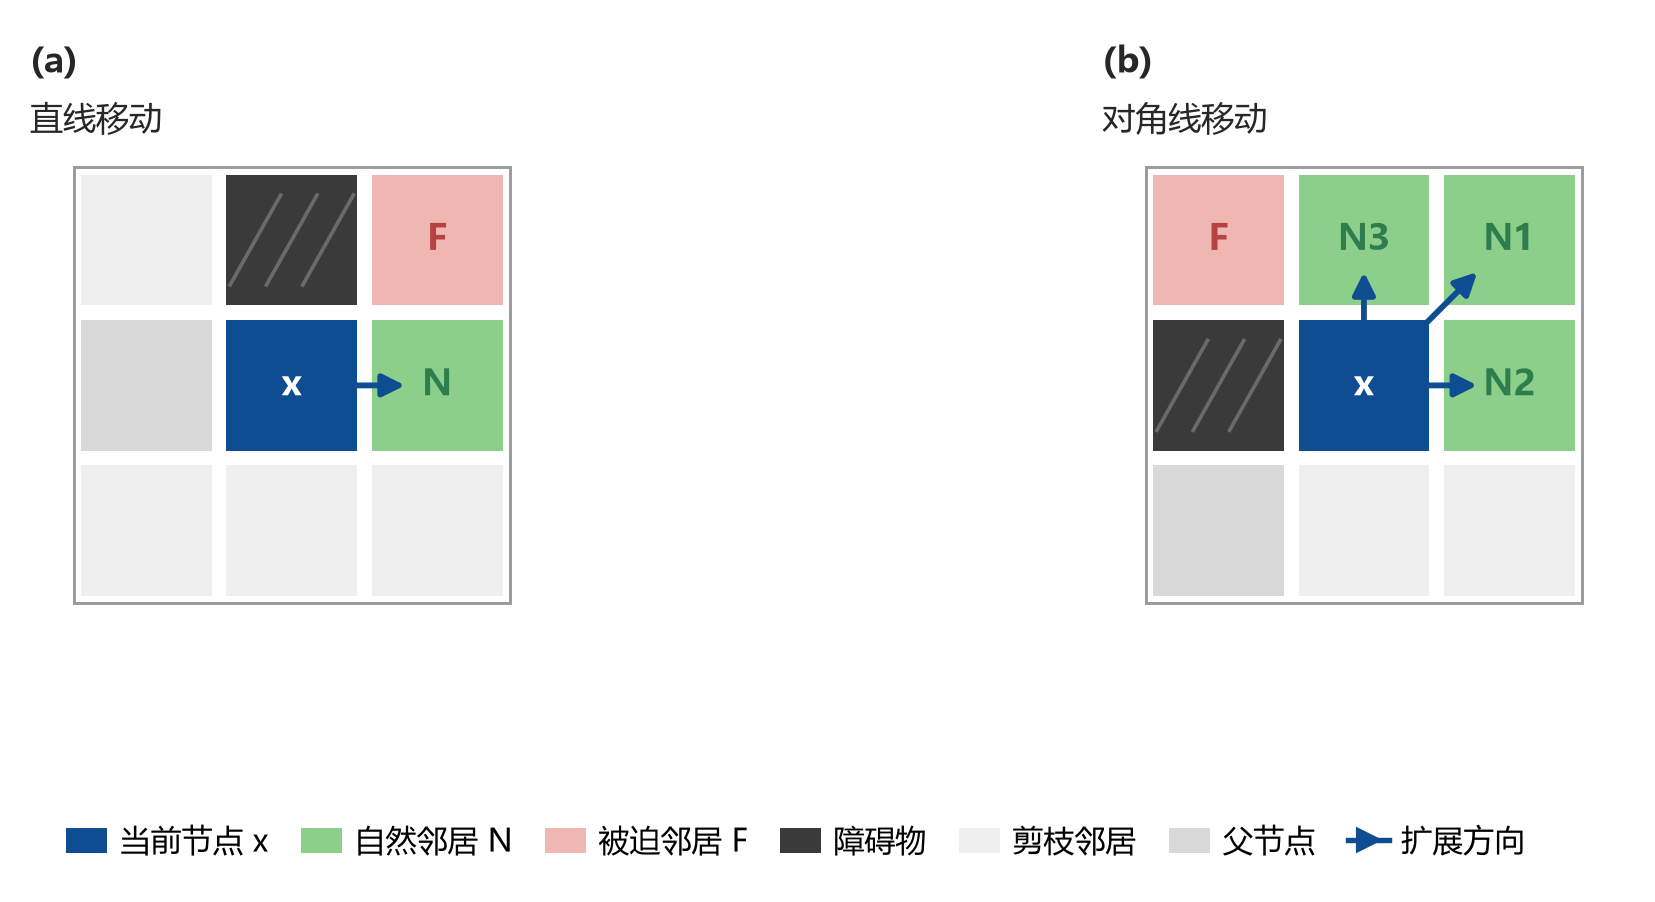
\includegraphics[width=2.5in]{figures/fig01_jps_pruning}
\caption{JPS邻居剪枝规则示意图。}
\label{fig:jps_pruning}
\end{figure}
\textbf{跳跃函数。} JPS的跳跃函数 $\mathrm{jump}(r, c, dr, dc)$ 从当前节点$(r, c)$出发，沿方向$(dr, dc)$逐步前进，直到满足以下三个终止条件之一：（1）到达目标节点；（2）遇到障碍物或地图边界（该方向不可通行）；（3）发现被迫邻居（当前位置因障碍物阻挡而需要强制转向）。跳跃过程中经过的中间节点不会被加入open set，从而显著减少了节点扩展数量。当遇到被迫邻居时，当前节点即为跳跃点，需要加入open set进行后续评估。
对于对角线方向的跳跃，算法会先沿对角线前进一步，然后分别沿水平和垂直分量方向执行直线跳跃。若任一方向的直线跳跃发现了被迫邻居或到达目标，则返回当前对角线位置作为跳跃点。
\textbf{路径成本计算。} 在$\mathrm{jump}$函数返回可达的下一个节点后，AStar\_v3\_1需要计算从当前节点到该跳跃点的实际移动成本。对于直线跳跃，成本等于跳跃的曼哈顿距离；对于对角线跳跃，成本等于对角线距离（每步对角线移动成本为$\sqrt{2}$）。算法~\ref{alg:jps}给出了JPS搜索过程的伪代码。
\begin{algorithm}[!t]
\caption{JPS-based A* search}
\label{alg:jps}
\begin{algorithmic}[1]
\REQUIRE occupancy grid map, start grid $S$, goal grid $G$
\ENSURE grid path $P = [S, \ldots, G]$, or failure
\STATE initialize $g(S) = 0$, $f(S) = h(S, G)$, and insert $S$ into the open set (a binary min-heap);
\WHILE{the open set is not empty}
\STATE $n \gets$ the node in the open set with the smallest $f$-value, breaking ties by the smaller $h$;
\IF{$n = G$}
\STATE reconstruct and return the grid path $P$;
\ENDIF
\STATE move $n$ into the closed set, and record its parent direction $\mathbf{d}_n$;
\STATE $D \gets$ the pruned successor directions of $n$ determined by $\mathbf{d}_n$ (all eight directions if $n = S$);
\FOR{each direction $\mathbf{d} \in D$}
\STATE $s \gets \mathrm{Jump}(n, \mathbf{d})$, the first jump point encountered along $\mathbf{d}$, or null;
\IF{$s = \mathrm{null}$ or $s$ is closed}
\STATE continue;
\ENDIF
\STATE $\mathrm{tent\_g} \gets g(n) + \mathrm{Cost}(n, s)$, where straight steps cost $1$ and diagonal steps cost $\sqrt{2}$;
\IF{$\mathrm{tent\_g} < g(s)$}
\STATE set the parent of $s$ to $n$, $g(s) \gets \mathrm{tent\_g}$, $f(s) \gets \mathrm{tent\_g} + h(s, G)$;
\STATE insert $s$ into the open set, or update its heap position if already present;
\ENDIF
\ENDFOR
\ENDWHILE
\IF{the open set is exhausted without reaching $G$}
\STATE fall back to standard A* (AStar\_v0);
\ENDIF
\end{algorithmic}
\end{algorithm}
\textbf{路径重建与对角拐点修正。} JPS搜索完成后，通过父节点指针从目标节点回溯至起点，并在相邻跳跃点之间沿直线插值补充被跳过的中间栅格，即可得到完整路径。然而，由于JPS的跳跃特性，重建路径中的对角线移动可能穿越障碍物拐角。为此，AStar\_v3\_1在路径重建阶段引入了对角拐点修正机制：当检测到对角线移动穿越障碍物角时，将其替换为沿栅格边界行走的L形路径（先走行再走列，或先走列再走行），从而避免与障碍物发生碰撞。修正后的路径严格沿栅格边界行进，保证了路径的可行性。
\textbf{算法降级机制。} JPS的剪枝规则依赖于均匀的栅格地图结构。在包含复杂障碍物分布的地图中，被迫邻居的产生频率增加，JPS的优势会被削弱，个别情况下对称性假设失效可能导致JPS搜索失败。为此，AStar\_v3\_1在JPS搜索耗尽开放集仍未找到路径时，自动回退至标准A*模式（AStar\_v0）重新搜索，以确保在存在可行解时总能找到路径。这一降级机制保证了算法的鲁棒性，使其能够适应不同复杂度的环境。
\subsubsection{打破平局策略}
当开放集中的多个节点具有相同的$f$值时，标准A*的选择顺序取决于具体实现（通常是先入先出或随机），本质上是任意的。然而，在$f$值相同的节点中，$h$值较小的节点意味着其实际代价$g = f - h$较大，即该节点距起点更远、更接近目标。优先扩展此类节点可将搜索方向导向目标，且不影响最优性保证。为此，AStar\_v3\_1采用``$f$值相同时优先选择$h$值更小的节点''的打破平局策略，二叉堆中的节点比较规则定义为：
\begin{equation}
\mathrm{compare}(n_1, n_2) =
\begin{cases}
n_1, & f(n_1) < f(n_2) \\
n_2, & f(n_1) > f(n_2) \\
n_1, & f(n_1) = f(n_2) \land h(n_1) < h(n_2) \\
n_2, & f(n_1) = f(n_2) \land h(n_1) > h(n_2)
\end{cases}
\label{eq:tbreak}
\end{equation}
该比较规则直接嵌入二叉堆的上浮（\texttt{bubbleUp}）与下沉（\texttt{bubbleDown}）操作中。
\textbf{物理意义。} 由评估函数$f(n) = g(n) + h(n)$可知，当两个节点的$f$值相同时，$g$值较大者$h$值较小。$g$值较大表示该节点距起点更远，而$h$值较小表示其更接近目标。优先扩展此类节点使搜索偏向目标方向，减少了远离目标区域的无效探索。由于$h$值在节点扩展时已经计算，此打破平局策略不产生额外计算开销。
\subsection{路径后处理}
\label{subsec:post}
JPS搜索得到的路径由栅格中心点序列组成，存在两个主要问题：路径包含冗余的中间点，且由离散的水平和垂直段组成导致平滑性不足。本节提出一种两阶段后处理流水线来解决这些问题。
\subsubsection{安全感知路径简化}
传统的路径简化方法（如拐角裁剪）直接连接路径上的非相邻节点，跳过中间点以减少路径点数量。然而，这类方法通常仅检查连接线段是否穿越障碍物，忽略了路径点与障碍物之间的安全裕度，在障碍物密集区域可能导致路径过于贴近障碍物。为此，本节提出一种安全距离感知的路径简化算法，其核心思想是在简化过程中保持路径与障碍物之间的最小安全距离。
该算法采用四步流程处理输入路径：
\textbf{第一步：拐点提取。} 从路径中识别方向发生变化的节点（即拐点）。对于路径中的每个中间节点，计算其与前后节点的连接方向。若前向连接方向与后向连接方向不同，则该节点标记为拐点。路径的起点和终点始终保留。
\textbf{第二步：贪心前向扫描。} 从当前拐点$C_i$出发，正向扫描所有后续拐点$C_j$（$j > i$），调用\textsc{IsLineFree}逐一验证线段$C_i \to C_j$是否满足安全距离约束，并记录\textbf{最远的}可达拐点$j^{*}$。该拐点成为新的锚点，其间的所有拐点被跳过。这种贪心策略在保证安全性的前提下最大化了单步简化程度。
\textbf{第三步：中间点探索。} 贪心步骤确定最远可达拐点$j^{*}$后，算法检查被跳过的拐点$k$（$i < k < j^{*}$）能否通过安全线段直达更远处的拐点$j'$（$j' > j^{*}$）。对每一对满足安全约束的$(k, j')$，算法计算并比较两条路径的代价。若存在这样的中间拐点，则可能得到比纯贪心更短的简化路径。
\textbf{第四步：路径比较。} 比较两条路径的长度：路径A（贪心）为$d(C_i, C_{j^{*}}) + d(C_{j^{*}}, C_{j'})$，即先到达$j^{*}$再继续到$j'$；路径B（经中间点）为$d(C_i, C_k) + d(C_k, C_{j'})$，即跳过$j^{*}$改经$k$路由。若路径B更短，则保留中间拐点$C_k$；否则仅保留贪心结果$C_{j^{*}}$。这一比较确保中间点探索不会以牺牲路径效率为代价。
安全性检查函数$\textsc{IsLineFree}(p_1, p_2, \mathrm{map}, d_{\mathrm{safe}})$的实现基于逐栅格采样：从$p_1$到$p_2$沿线段密集采样，对每个采样点计算其与最近障碍物栅格边界的距离。只要任意采样点的距离小于安全阈值$d_{\mathrm{safe}}$，即判定该连接不安全。点到栅格边界的距离计算公式为：
\begin{align}
d_x &= \max\left(0,\; |p_r - c_r| - 0.5\right), \nonumber\\
d_y &= \max\left(0,\; |p_c - c_c| - 0.5\right)
\label{eq:dxymax}\\
d(p, \mathrm{cell}) &= \sqrt{d_x^2 + d_y^2}
\label{eq:dist}
\end{align}
其中，$p = (p_r, p_c)$为连续坐标下的采样点，$c = (c_r, c_c)$为障碍物栅格的中心坐标，栅格占据矩形区域$[c_r - 0.5, c_r + 0.5] \times [c_c - 0.5, c_c + 0.5]$。$\max(0, \cdot)$算子处理采样点在某坐标轴上已落入栅格水平或垂直范围内的情况。当$d(p, \mathrm{cell}) < d_{\mathrm{safe}}$时，表示采样点已进入障碍物栅格的安全禁区。安全距离阈值$d_{\mathrm{safe}}$设置为机器人半径$r_{\mathrm{robot}} = 0.2$加上$0.2$的裕度（即$d_{\mathrm{safe}} = 0.4$），保证路径中心线到障碍物的距离不小于机器人半径，从而保证无碰撞。算法~\ref{alg:simplify}给出了路径简化算法的伪代码。
\begin{algorithm}[!t]
\caption{Safety-distance-aware path simplification}
\label{alg:simplify}
\begin{algorithmic}[1]
\REQUIRE grid path $P = [P_1, \ldots, P_N]$, occupancy grid, safety margin $d_{\mathrm{safe}}$
\ENSURE simplified path $P_s$ ($|P_s| \leq N$)
\STATE $C \gets$ the corner points of $P$ where the direction changes, plus the two endpoints;
\STATE $P_s \gets [C_1]$; $\; i \gets 1$;
\WHILE{$i < |C|$}
\STATE $j^{*} \gets$ the farthest corner reachable from $C_i$ by a collision-free segment; \quad\textit{greedy forward scan}
\IF{$j^{*} = |C|$}
\STATE append $C_{|C|}$ to $P_s$ and break;
\ENDIF
\STATE $(k^{*}, j') \gets$ among all skipped corners $k$ ($i < k < j^{*}$) and farther corners $j$ ($j^{*} < j \leq |C|$), the pair with the largest $j$ such that the segment $C_k \to C_j$ is collision-free;
\IF{$k^{*}$ exists and $d(C_i, C_{k^{*}}) + d(C_{k^{*}}, C_{j'}) < d(C_i, C_{j^{*}}) + d(C_{j^{*}}, C_{j'})$}
\STATE append $C_{k^{*}}$ and $C_{j'}$ to $P_s$, and set $i \gets j'$; \quad\textit{route through the intermediate corner}
\ELSE
\STATE append $C_{j^{*}}$ to $P_s$, and set $i \gets j^{*}$;
\ENDIF
\ENDWHILE
\STATE \RETURN $P_s$;
\end{algorithmic}
\end{algorithm}
安全性检查函数\textsc{IsLineFree}的伪代码如算法~\ref{alg:islinefree}所示。搜索半径$d_{\max}$设置为$\lceil d_{\mathrm{safe}} + 0.5 \rceil$，因为超出此距离的栅格不可能与采样点的安全距离产生交集。
\begin{algorithm}[!t]
\caption{IsLineFree (collision check with safety margin)}
\label{alg:islinefree}
\begin{algorithmic}[1]
\REQUIRE segment endpoints $p_1$, $p_2$ (grid coordinates), occupancy grid, safety margin $d_{\mathrm{safe}}$
\ENSURE true if the segment keeps distance $\geq d_{\mathrm{safe}}$ from every obstacle, false otherwise
\STATE $\ell \gets \max(|p_1.r - p_2.r|,\; |p_1.c - p_2.c|)$;
\STATE $N_s \gets \max(\lceil 10 \cdot \ell \rceil, 30)$; \quad\textit{number of dense sample points}
\STATE $d_{\max} \gets \lceil d_{\mathrm{safe}} + 0.5 \rceil$; \quad\textit{search radius in cells}
\FOR{$k = 0$ to $N_s$}
\STATE $p \gets p_1 + (k / N_s) \cdot (p_2 - p_1)$; \quad\textit{sample point in continuous coordinates}
\FOR{each cell $(r, c)$ within Chebyshev distance $d_{\max}$ of $p$}
\IF{$(r, c)$ is occupied}
\STATE $d \gets$ the distance from $p$ to the boundary of cell $(r, c)$; \quad\textit{see Eqs.~\eqref{eq:dxymax}--\eqref{eq:dist}}
\IF{$d < d_{\mathrm{safe}}$}
\STATE \RETURN false;
\ENDIF
\ENDIF
\ENDFOR
\ENDFOR
\STATE \RETURN true;
\end{algorithmic}
\end{algorithm}
\subsubsection{弧长参数化三次样条平滑}
路径简化后的路径虽已去除冗余点，但仍由直线段连接组成，在拐点处存在曲率突变，不适合全向机器人的平滑运动。本节采用三次样条插值对简化路径进行平滑处理。
传统的三次样条插值直接以路径点的索引作为参数进行拟合，当路径点间距不均匀时会导致曲线形状失真。为解决这一问题，本节采用弧长参数化方法，以路径点之间的累积欧氏距离作为参数，使参数空间与实际几何空间保持一致。平滑过程分为三个步骤：
\textbf{步骤一：稀疏段致密化。} 首先检测路径中相邻点间距超过2个栅格单位的线段。对于这些稀疏段，在两端点之间沿线段线性插值$\lfloor \ell / 2 \rfloor$个中间点。致密化的目的是为样条曲线提供足够的控制点，防止曲线在长直段处因控制点不足而产生的过冲（Runge现象），避免曲线偏离预期折线甚至裁剪障碍物角点。
\textbf{步骤二：弧长参数化。} 设致密化后的路径点序列为$\{P_0, P_1, \ldots, P_M\}$，其中$P_i = (x_i, y_i)$为连续坐标。计算各点的累积弦长（弧长）参数：
\begin{equation}
s_0 = 0, \quad s_i = s_{i-1} + \|P_i - P_{i-1}\|_2, \quad i = 1, 2, \ldots, M
\label{eq:arclen}
\end{equation}
然后分别以$s$为自变量对$x(s)$和$y(s)$进行三次样条插值，得到参数化曲线$(x(s), y(s))$。三次样条在每个子区间$[s_i, s_{i+1}]$上为三次多项式，保证一阶和二阶导数连续，从而确保曲线的曲率连续性。
\textbf{步骤三：等弧长重采样。} 以密度$\rho = 10$（每段插入10个点）沿弧长参数$s$均匀采样，生成最终的平滑路径点序列。由于$s$与实际几何距离近似线性关系，等弧长采样保证了路径点在空间中的均匀分布，避免了传统等参数采样在曲率大处点密、曲率小处点疏的问题。算法~\ref{alg:smooth}给出了平滑算法的伪代码。
\begin{algorithm}[!t]
\caption{Arc-length parameterized cubic spline smoothing}
\label{alg:smooth}
\begin{algorithmic}[1]
\REQUIRE grid path $P = [P_1, \ldots, P_N]$, density $\rho$ (default $10$)
\ENSURE smoothed continuous path $Q = [Q_1, \ldots, Q_M]$ in $[x, y]$
\STATE convert each grid point $P_i = (r_i, c_i)$ to continuous coordinates $(x_i, y_i) = (c_i - 0.5,\; r_i - 0.5)$;
\FOR{each consecutive pair whose segment length exceeds $2$}
\STATE insert $\lfloor \mathrm{length} / 2 \rfloor$ equally spaced intermediate points along the segment; \quad\textit{densification to prevent spline overshoot}
\ENDFOR
\STATE compute the cumulative chord length $t_1 = 0$, $t_i = t_{i-1} + \|P_i - P_{i-1}\|_2$; \quad\textit{arc-length parameter}
\STATE remove duplicate $t$ values to keep strict monotonicity;
\STATE fit cubic splines $x(t)$ and $y(t)$ through the densified points;
\STATE sample $x(t)$ and $y(t)$ at $\rho$ points per segment to obtain $Q$;
\STATE \RETURN $Q$;
\end{algorithmic}
\end{algorithm}
\subsubsection{流水线集成}
上述后处理操作以流水线方式集成：JPS搜索（算法~\ref{alg:jps}）输出原始栅格路径 $\to$ SimplifyPath（算法~\ref{alg:simplify}）去除冗余点 $\to$ SmoothPath（算法~\ref{alg:smooth}）生成平滑的连续坐标路径。整个流水线在SimulationManager中一次性完成，输出的路径既满足安全性约束，又具有良好的平滑性，可直接用于机器人的运动跟踪。
这种两阶段设计的合理性在于：路径简化和样条平滑分别解决了路径质量的两个不同维度。简化减少了路径点数量（降低了后续计算的复杂度），同时通过安全距离约束保证了路径的安全裕度；平滑则将离散的栅格路径转化为连续曲线，使机器人能够以平滑的运动轨迹跟踪路径。若跳过简化直接进行平滑，样条曲线需要处理大量冗余的控制点，不仅计算成本更高，还可能因控制点过于密集而产生不稳定的曲线形状。消融实验（表~\ref{tab:ablation}）的结果也验证了这一设计的有效性。路径后处理前后对比如图~\ref{fig:pipeline}所示。
\begin{figure}[!t]
\centering
\subfloat[原始路径与简化后路径]{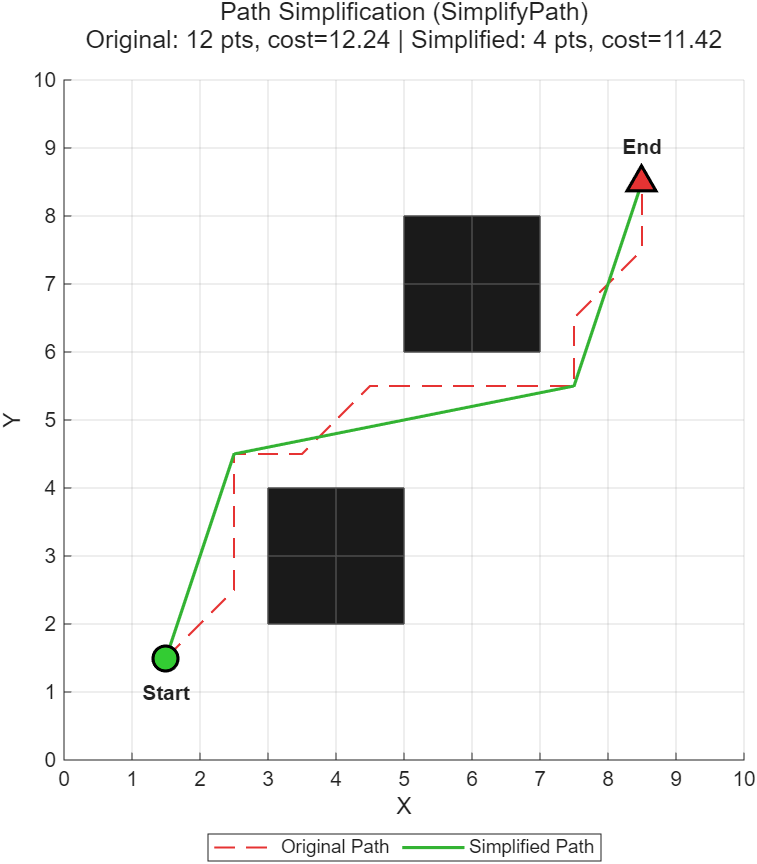
\includegraphics[width=1.55in]{figures/fig02a_simplify_raw}%
\label{fig:pipeline_a}}%
\hfil
\subfloat[简化后路径与平滑后路径]{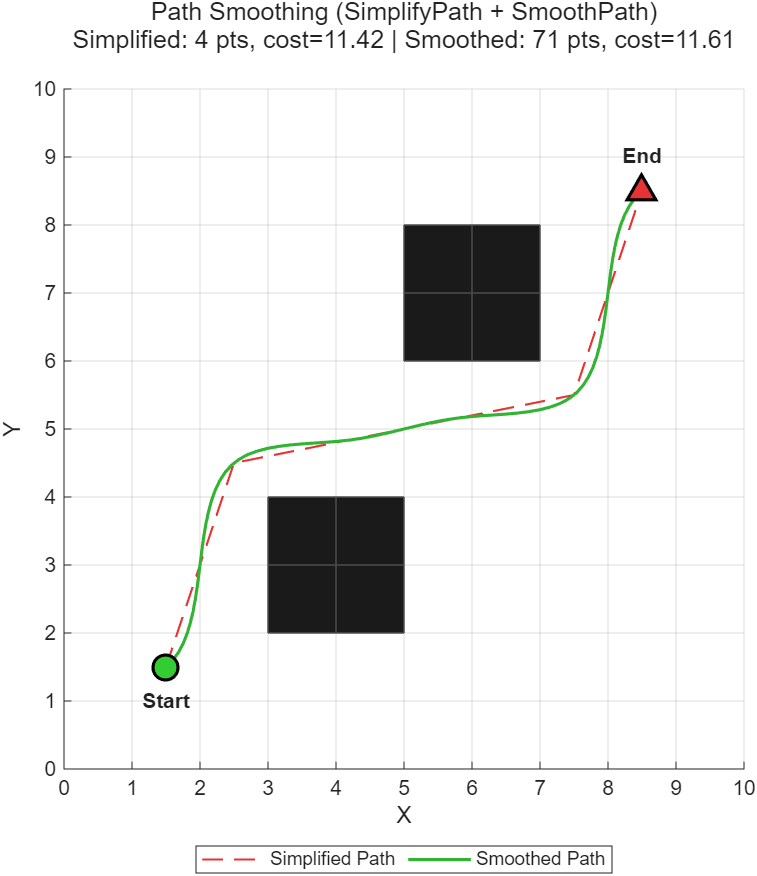
\includegraphics[width=1.55in]{figures/fig02b_smooth_raw}%
\label{fig:pipeline_b}}
\caption{路径通过管线各阶段的对比。}
\label{fig:pipeline}
\end{figure}
\subsection{改进的开放旅行商蚁群优化}
\label{subsec:aco}
本框架的第二层在全局规划层产生的代价矩阵上求解开放旅行商问题。给定由固定起点$S$、$K$个中间目标点$\{T_1, \dots, T_K\}$和固定终点$G$组成的$N$个点，目标是找到使总路径代价最小的$K$个目标点排列。我们在蚁群优化（ACO）元启发式方法基础上引入六个集成机制：（1）虚拟节点法，将开放旅行商问题转化为标准闭环旅行商问题；（2）最大-最小蚁群系统（MMAS）信息素管理及动态更新边界；（3）蚁群系统（ACS）风格的伪随机比例转移规则，平衡探索与利用；（4）以$k$近邻候选列表加速的可变邻域下降（VND）局部搜索；（5）S形渐进调度策略，将搜索从探索主导逐渐转向利用主导；（6）自适应停止准则。
\subsubsection{虚拟节点法编码开放旅行商问题}
\label{subsec:virtual}
\textbf{动机。} 在标准闭环旅行商问题中，解为哈密顿回路，任意城市均可作为起始点。在我们的问题中，起点$S$和终点$G$是由任务规格确定的物理上不同的位置——例如无人公交的始发站和终点站。这两个点必须出现在每个候选解的固定位置（首尾），优化仅针对$K$个中间目标点的排序进行。将所有$N$个点对称排列的朴素编码会产生将起点/终点混入路径中间的无效路径；而将起点/终点固定在路径两端的边界固定编码将其排除在信息素模型和局部搜索之外，限制了算法对完整解的优化能力。
\textbf{机制。} 我们采用虚拟节点（哑节点）法将开放旅行商问题转化为标准闭环旅行商问题，该技术在开放车辆路径问题中被广泛采用\cite{ref31,ref32}。引入虚拟节点$V = N + 1$，构造$(N+1) \times (N+1)$的扩展代价矩阵$\mathbf{D}_{\mathrm{ext}}$：
\begin{equation}
\mathbf{D}_{\mathrm{ext}}(i, j) =
\begin{cases}
0, & \{i, j\} = \{V, 1\} \text{（虚拟节点 $\leftrightarrow$ 起点）} \\
0, & \{i, j\} = \{V, N\} \text{（虚拟节点 $\leftrightarrow$ 终点）} \\
\mathrm{BIG}, & i = V \text{ 或 } j = V,\ \text{且 } \{i, j\} \cap \{1, N\} = \varnothing \\
\mathbf{D}(i, j), & \text{其他}
\end{cases}
\label{eq:dext}
\end{equation}
其中$\mathrm{BIG} = 2(N+1) \cdot \max_{i,j} \mathbf{D}(i,j)$为严格大于任何可行回路代价的惩罚值，确保虚拟节点在任何近优回路中不直接连接任何中间目标点。虚拟节点与起点/终点之间的零代价边使虚拟节点对路径代价``不可见''，而与中间目标点之间的惩罚边强制虚拟节点仅与起点和终点相邻。
蚁群优化求解器在扩展代价矩阵$\mathbf{D}_{\mathrm{ext}}$上作为标准闭环旅行商问题运行：所有蚂蚁构建访问所有$N+1$个节点（包括虚拟节点）的完整哈密顿回路，信息素矩阵$\bm{\tau}$覆盖完整的$(N+1) \times (N+1)$空间。求解器收敛后，通过以下步骤从最优回路中提取开放路径访问顺序：
\begin{enumerate}
\item 定位回路中的虚拟节点$V$。
\item 移除$V$并按回路顺序读取剩余$N$个节点。
\item 调整方向使起点（1）出现在首位、终点（$N$）出现在末位。
\end{enumerate}
该转换相对边界固定编码有三个优势：（a）起点和终点节点完整参与信息素模型和局部搜索，而非被排除为固定边界；（b）所有标准闭环旅行商算子（2-opt、重定位、交换）统一适用，无需特殊边界处理；（c）代价评估为$\mathbf{D}_{\mathrm{ext}}$上的简单回路求和，避免了单独边界代价项的需求。
启发式可见度矩阵$\bm{\eta}$在扩展空间上定义。对涉及虚拟节点的点对，到起点/终点的零代价边赋予大启发式值$\eta_{V,1} = \eta_{1,V} = \eta_{V,N} = \eta_{N,V} = \mathrm{BIG}$，强烈吸引虚拟节点连接其所需邻居。对其他点对：
\begin{equation}
\eta_{ij} =
\begin{cases}
1 / \mathbf{D}_{\mathrm{ext}}(i,j), & \mathbf{D}_{\mathrm{ext}}(i,j) > 0 \text{ 且 } \mathbf{D}_{\mathrm{ext}}(i,j) < \infty \\
0, & \text{其他}
\end{cases}
\label{eq:eta}
\end{equation}
闭合回路$\bm{\sigma} = (\sigma_1, \sigma_2, \dots, \sigma_{N+1})$的代价为：
\begin{equation}
C(\bm{\sigma}) = \sum_{k=1}^{N} \mathbf{D}_{\mathrm{ext}}(\sigma_k, \sigma_{k+1}) + \mathbf{D}_{\mathrm{ext}}(\sigma_{N+1}, \sigma_1)
\label{eq:tourcost}
\end{equation}
\subsubsection{具有动态边界的最大-最小蚁群系统信息素更新}
\textbf{动机。} 在基本蚁群系统中，所有蚂蚁在其完整路径上沉积信息素，当少数蚂蚁偶然找到中等质量的路径时可能导致搜索过早集中于次优解。反之，无边界的过度蒸发可能使信息素值在除主导边之外的所有边上趋近于零，将种群困在局部最优。最大-最小蚁群系统（MMAS）\cite{ref23}通过以下方式解决这两个问题：（a）将信息素限制在显式区间$[\tau_{\min}, \tau_{\max}]$内，防止支配和灭绝；（b）聚焦于最优性能解的沉积。
\textbf{机制。} 每次迭代，所有信息素值首先进行蒸发：
\begin{equation}
\tau_{ij} \leftarrow (1 - \rho) \cdot \tau_{ij} \quad \forall i, j \in \{1, \dots, N+1\}
\label{eq:evap}
\end{equation}
其中$\rho = 0.25$为蒸发率。蒸发后，在两个解层次的边上沉积信息素：
\textbf{迭代最优沉积。} 当代最优蚂蚁在其回路的所有边上沉积信息素：
\begin{equation}
\tau_{ij} \leftarrow \tau_{ij} + \frac{Q}{C_{\mathrm{iter}}} \quad \forall (i, j) \in \mathrm{edges}(\bm{\sigma}_{\mathrm{iter-best}})
\label{eq:deposititer}
\end{equation}
\textbf{全局最优精英沉积。} 搜索开始以来找到的最优回路也获得沉积，强化全局主导解：
\begin{equation}
\tau_{ij} \leftarrow \tau_{ij} + \frac{Q}{C_{\mathrm{global}}} \quad \forall (i, j) \in \mathrm{edges}(\bm{\sigma}_{\mathrm{global-best}})
\label{eq:depositglob}
\end{equation}
其中$Q = 225$为沉积常数，$C$为回路代价。沉积量与回路代价成反比，因此更短（更优）的回路沉积更强的信息素。两个沉积级别同时应用于对称对$(j, i)$，保持无向信息素模型。
沉积后，所有信息素值被限幅到$[\tau_{\min}, \tau_{\max}]$区间，其边界根据当前全局最优动态更新：
\begin{align}
\tau_{\max} &= \frac{1}{\rho \cdot C_{\mathrm{global}}}
\label{eq:taumax}\\
\tau_{\min} &= \frac{\tau_{\max}}{N+1} = \frac{1}{\rho \cdot (N+1) \cdot C_{\mathrm{global}}}
\label{eq:taumin}
\end{align}
并设有硬下限$\tau_{\min} \geq 10^{-6}$以防止低频边上信息素完全灭绝。边界的动态更新至关重要：随着搜索发现更优回路（$C_{\mathrm{global}}$减小），$\tau_{\max}$增大，允许算法对其当前最优解表达更强的置信。反之，比率$\tau_{\min}/\tau_{\max} = 1/(N+1)$维持最小与最大信息素之间的恒定相对间隔，无论绝对尺度如何，都为所有边保持基线探索概率。
初始信息素矩阵设为均匀值$\tau_0 = 0.1$，表示搜索经验积累前的中性先验。
\subsubsection{蚁群系统风格的伪随机转移规则}
\textbf{动机。} 在标准蚁群系统中，每只蚂蚁通过纯概率轮盘选择从未访问的候选集中选择下一节点。此方法探索性强，在距离启发式提供可靠引导的结构化问题上收敛缓慢。蚁群系统（ACS）\cite{ref22}通过伪随机比例规则解决此问题：以可控概率，蚂蚁贪心地选择最优候选；否则通过标准概率机制探索。这平衡了收敛需求（利用）与避免局部最优的需求（探索）。
\textbf{机制。} 当蚂蚁在当前节点$u$从未访问候选集$\mathcal{U}$中选择下一节点时，首先计算每个候选的得分：
\begin{equation}
\mathrm{score}(v) = (\tau_{uv})^{\alpha} \cdot (\eta_{uv})^{\beta} \quad \forall v \in \mathcal{U}
\label{eq:score}
\end{equation}
其中$\alpha = 1$和$\beta = 2.0$分别为信息素和启发式权重指数。转移决策遵循：
\begin{equation}
v_{\mathrm{next}} =
\begin{cases}
\arg\max_{v \in \mathcal{U}} \; \mathrm{score}(v), & \text{概率 } q_0 \\
\mathrm{roulette}(\mathcal{U}, \mathrm{score}), & \text{概率 } 1 - q_0
\end{cases}
\label{eq:trans}
\end{equation}
其中$q_0 = 0.45$为利用概率。在利用情形中，蚂蚁确定性地选择得分最高的候选——等价于贪心最优步。在探索情形中，蚂蚁执行轮盘选择，每个候选$v$以$\mathrm{score}(v) / \sum_{u \in \mathcal{U}} \mathrm{score}(u)$的概率被选中。若所有得分为零（所有剩余节点不可达），随机选择一个未访问候选作为回退。
$q_0 = 0.45$意味着平均而言，45\%的构建步使用贪心选择加速收敛，而55\%通过随机探索维持多样性。此比率的设定基于障碍约束代价矩阵的结构化特性——点对间距离通常表现出空间局部性，启发式$\bm{\eta}$携带可靠信息。
\subsubsection{具有候选列表加速的可变邻域下降局部搜索}
\label{subsec:vnd}
\textbf{动机。} 蚂蚁构建的路径虽然受信息素和启发式信息引导，但不能保证局部最优。对每代最优蚂蚁施加局部搜索，通过系统性地探索邻域排列来精化解。可变邻域下降（VND）\cite{ref24}依次应用多个邻域结构，每种捕捉不同类型的路径变换，循环直至无结构能产生进一步改进。混合MMAS-VND和ACS-VND方案在车辆路径问题中已展现出强劲性能\cite{ref25}。然而，标准VND对每个算子检查$O(K^2)$邻域，在大规模实例上成为计算瓶颈。此外，大多数此类检查的移动是无效的——远距节点的候选对不太可能产生改进的2-opt交换。
\textbf{机制。} 我们的VND在所有$N+1$个节点（包括虚拟节点）的闭合回路上操作，按固定顺序采用三个邻域算子：
\begin{enumerate}
\item \textbf{2-opt}：反转路径的连续子序列，用$(u, v)$和$(u^{+}, v^{+})$替换$(u, u^{+})$和$(v, v^{+})$。这消除欧氏型代价结构中的路径交叉。
\item \textbf{重定位}：从当前位置提取单个节点并重新插入到回路中的不同位置，平移中间节点。这修正节点属于路径不同区域的局部错序。
\item \textbf{交换}：交换两个节点的位置，保持所有其他节点固定。这处理两个节点被分配到彼此最优位置的情况。
\end{enumerate}
三个算子在VND循环中采用首次改进（FI）策略：2-opt反复应用直至无改进，然后是重定位，然后是交换。若任一算子产生改进，循环重置回2-opt并重复。当三个算子连续未能改进解时搜索终止。
\textbf{候选列表加速。} 关键效率改进是使用预计算的候选列表剪枝无前景的邻域评估，该策略在旅行商问题局部搜索中已被广泛采用\cite{ref26}。对扩展问题中的每个$N+1$节点，我们基于扩展代价矩阵$\mathbf{D}_{\mathrm{ext}}$预计算$k = 9$个最近邻，并将其存储为布尔矩阵$\mathbf{C}$，其中$\mathbf{C}(i, j) = \mathrm{true}$表示节点$j$是节点$i$的$k$个最近邻之一。三个VND算子的剪枝规则如下：
\begin{itemize}
\item \textbf{2-opt剪枝}：仅当所提议的新边$(u, v)$或$(u^{+}, v^{+})$中至少一对是候选邻居时，才评估候选2-opt移动。
\item \textbf{重定位剪枝}：仅当被移动节点$v$是其新相邻节点之一$p$或$p^{+}$的候选邻居时，才评估将节点$v$插入$p$之后的移动。
\item \textbf{交换剪枝}：仅当被交换的两个节点$a$和$b$互为候选邻居时，才评估交换操作。
\end{itemize}
剪枝在设计上是保守的：仅当移动的新边均不涉及候选对时才跳过评估——这是移动不太可能改进回路的强但非绝对信号。较小的候选列表大小$k = 9$旨在积极过滤评估，同时保留最有可能的局部移动；这在扩展代价矩阵表现出强空间结构时尤为有效，仅有邻近节点可能参与改进的边交换。
\textbf{复杂度。} 无剪枝时，每个VND算子检查$O((N+1)^2)$个候选移动。通过候选列表剪枝，每个节点仅参与$O(k)$次邻域检查，将每算子复杂度降至$O((N+1) \cdot k)$。对于典型问题规模（$N \approx 100$，$k = 9$），这代表约$10\times$的缩减；差距随$N$呈二次增长。
算法~\ref{alg:vnd}给出了候选列表加速VND的伪代码。
\begin{algorithm}[!t]
\caption{Candidate-list-accelerated variable neighborhood descent}
\label{alg:vnd}
\begin{algorithmic}[1]
\REQUIRE closed tour $\bm{\sigma} = [\sigma_1, \dots, \sigma_{N+1}]$, extended cost matrix $\mathbf{D}_{\mathrm{ext}}$, candidate boolean matrix $\mathbf{C}$
\ENSURE improved tour $\bm{\sigma}$ and its cost
\STATE $\mathrm{cost} \gets$ the cost of tour $\bm{\sigma}$ under $\mathbf{D}_{\mathrm{ext}}$;
\REPEAT
\STATE $\mathrm{improved} \gets$ false;
\STATE $[\bm{\sigma}, \mathrm{cost}, \mathrm{ok}] \gets$ apply the 2-opt operator with candidate-list pruning (first-improvement);
\STATE $\mathrm{improved} \gets \mathrm{improved}$ or ok;
\STATE $[\bm{\sigma}, \mathrm{cost}, \mathrm{ok}] \gets$ apply the relocate operator with candidate-list pruning;
\STATE $\mathrm{improved} \gets \mathrm{improved}$ or ok;
\STATE $[\bm{\sigma}, \mathrm{cost}, \mathrm{ok}] \gets$ apply the swap operator with candidate-list pruning;
\STATE $\mathrm{improved} \gets \mathrm{improved}$ or ok;
\UNTIL{$\mathrm{improved} = \mathrm{false}$}
\STATE $\mathrm{cost} \gets$ the exact cost of the final tour $\bm{\sigma}$;
\STATE \RETURN $\bm{\sigma}$, $\mathrm{cost}$;
\end{algorithmic}
\end{algorithm}
邻域算子（TwoOptClosed、RelocateClosed、SwapClosed）各自采用首次改进策略——首个发现降低回路代价的移动被立即接受，算子返回。闭合回路拓扑要求交换算子特殊处理：当交换跨越回路闭合边的两个相邻节点（即回路最后一个和第一个元素）时，标准线性邻接逻辑必须考虑环绕连接。VND邻域搜索序列如图~\ref{fig:vnd_flow}所示。
\begin{figure}[!t]
\centering
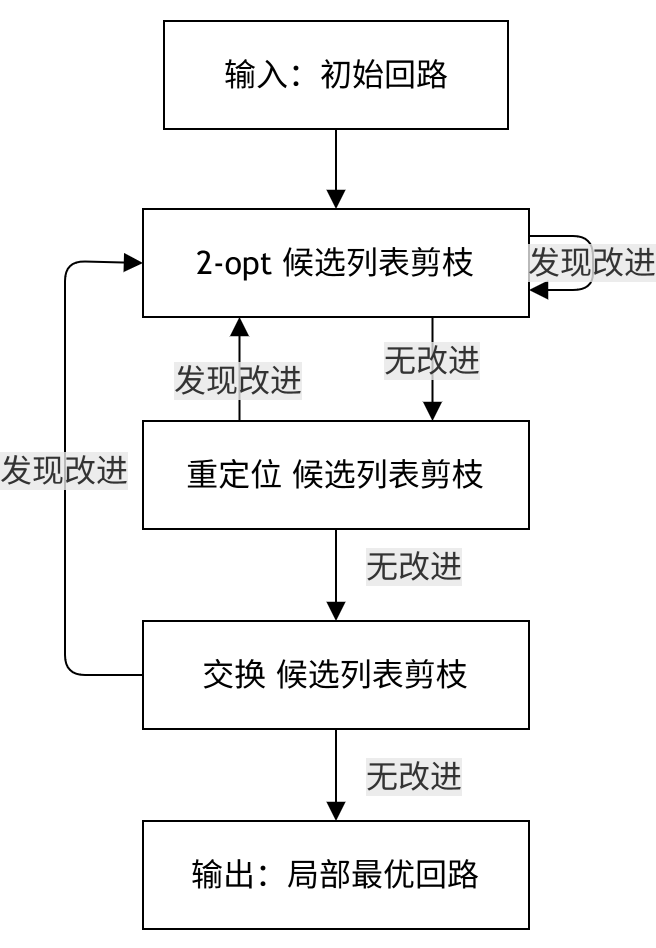
\includegraphics[width=2.2in]{figures/fig03_vnd_flow}
\caption{VND邻域搜索序列流程图。}
\label{fig:vnd_flow}
\end{figure}
\subsubsection{S形渐进局部搜索调度}
\label{subsec:sigmoid}
\textbf{动机。} 即使有候选列表加速，VND局部搜索的计算代价意味着在每代对每只蚂蚁施加局部搜索会浪费早期世代的资源——此时种群尚未识别出搜索空间中有前景的区域。反之，在后期世代中，当信息素已收敛至高质量解时，密集局部搜索对精细调优至关重要。在整个运行过程中对固定比例的蚂蚁施加局部搜索是次优的：比例过低导致收敛停滞，比例过高则在低质量路径上浪费计算。
\textbf{机制。} 我们根据S形（sigmoid）函数在迭代预算内调度接收VND局部搜索的蚂蚁比例：
\begin{equation}
\mathrm{optRatio}(t) = y_{\min} + (y_{\max} - y_{\min}) \cdot \frac{t^{a}}{t^{a} + (1 - t)^{a}}
\label{eq:sigmoid}
\end{equation}
其中$t = (\mathrm{iter} - x_L) / (x_R - x_L)$为转换区间$[x_L, x_R] = [0, 30]$内的归一化迭代位置。参数为：$y_{\min} = 0.0$（最开始无局部搜索），$y_{\max} = 0.4$（后期最多40\%的蚂蚁接收局部搜索），$a = 2.0$（S形曲线陡度）。$x_L$之前，$\mathrm{optRatio} = y_{\min}$；$x_R$之后，$\mathrm{optRatio} = y_{\max}$；区间内比率遵循平滑sigmoid过渡。
S形曲线提供三个理想特性：（1）早期迭代（$\mathrm{optRatio} \approx 0$），种群广泛探索而不承担局部搜索的计算代价，纯依赖构建层面的多样化；（2）过渡阶段，优化蚂蚁比例逐渐增加，允许信息素适应改进的解；（3）后期迭代（$\mathrm{optRatio} = 0.4$），相当比例的蚂蚁接收局部搜索，同时部分蚂蚁继续通过构建探索，维持多样性。转换区间$[0, 30]$有意设置较短：S形曲线尽早达到最大值，反映了在基本信息素结构建立后（约30次迭代后）密集局部搜索从一开始就有效的观察。S形$\mathrm{optRatio}(t)$曲线如图~\ref{fig:sigmoid}所示。
\begin{figure}[!t]
\centering
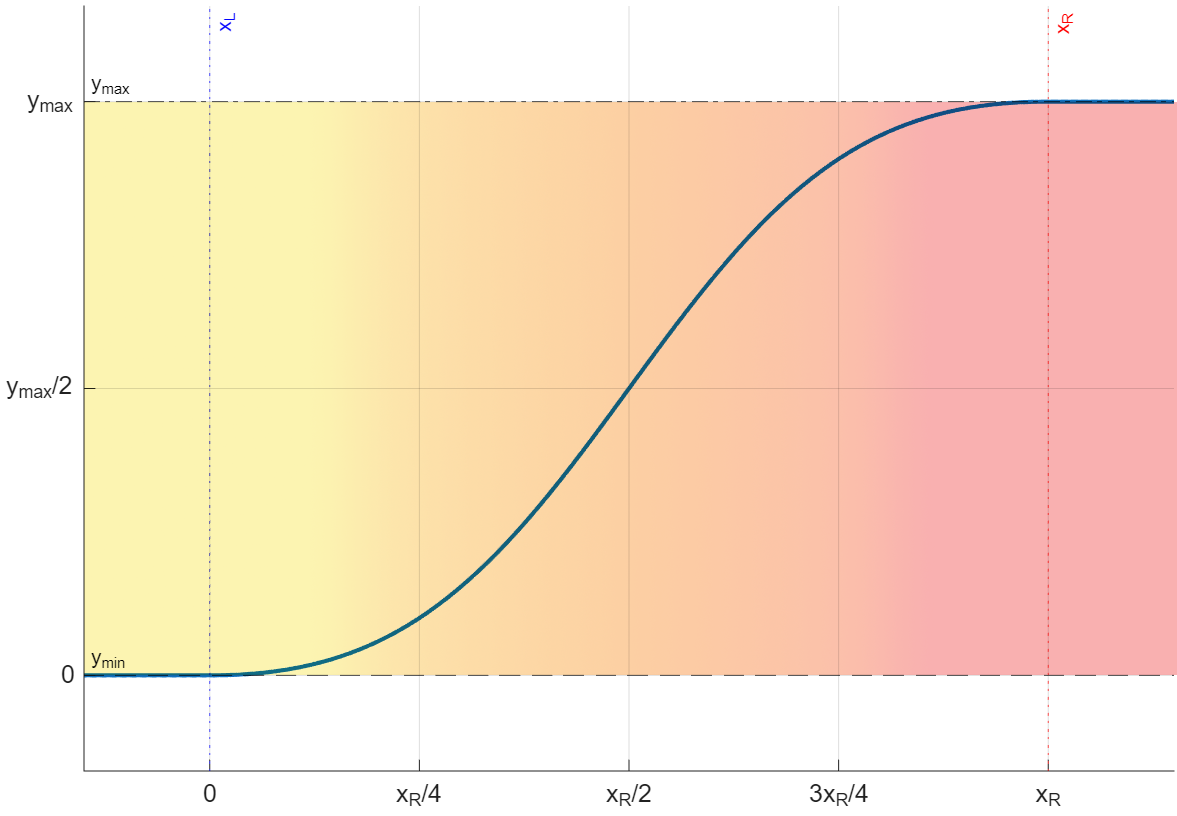
\includegraphics[width=2.5in]{figures/fig04_sigmoid}
\caption{S形$\mathrm{optRatio}(t)$关于迭代次数的曲线图。}
\label{fig:sigmoid}
\end{figure}
\textbf{局部搜索蚂蚁选择。} 确定接收局部搜索的蚂蚁数量$n_{\mathrm{opt}} = \lceil n_{\mathrm{ants}} \cdot \mathrm{optRatio} \rceil$后，选择哪些具体蚂蚁接收优化采用精英-随机混合策略：
\begin{align}
n_{\mathrm{elite}} &= \lceil n_{\mathrm{opt}} \cdot r_{\mathrm{elite}} \rceil
\label{eq:nelite}\\
n_{\mathrm{random}} &= n_{\mathrm{opt}} - n_{\mathrm{elite}}
\label{eq:nrandom}
\end{align}
其中$r_{\mathrm{elite}} = 0.7$（局部搜索预算的前70\%分配给排名最高的蚂蚁），剩余$n_{\mathrm{random}}$只蚂蚁从非精英池中随机选择。此选择确保最优解被精化（精英利用），同时少数随机选择的蚂蚁路径被优化，可能发现精英池忽略的搜索空间中其他高质量区域（受控探索）。
\subsubsection{自适应停止准则}
\textbf{动机。} 最大迭代次数$n_{\mathrm{iter}} = 800$保守地设定以适应困难问题实例。在较易实例上，种群可能远早于此收敛，继续运行浪费计算而不改进解。反之，过早终止有遗漏最优解的风险。自适应停止机制应检测真正的收敛，同时防止因暂时停滞导致的过早终止。
\textbf{机制。} 监测两个互补的收敛指标：
\textbf{条件1——种群同质性。} 当蚁群收敛至搜索空间的狭窄区域时，蚂蚁间的代价方差变得很小。我们通过每代蚂蚁代价的变异系数（CV）衡量：
\begin{equation}
\mathrm{CV} = \frac{\sigma_{\mathrm{costs}}}{\mu_{\mathrm{costs}}}
\label{eq:cv}
\end{equation}
其中$\sigma_{\mathrm{costs}}$和$\mu_{\mathrm{costs}}$分别为当代所有蚂蚁回路代价的标准差和均值。若$\mathrm{CV} < 0.001$，种群被视为同质——所有蚂蚁产生几乎相同质量的回路，进一步迭代不太可能发现新解。
\textbf{条件2——最优解停滞。} 即使种群保持多样，全局最优回路也可能陷入局部最优。我们跟踪全局最优代价未改进的连续迭代次数。若停滞计数器达到$70$代，搜索终止。
\textbf{最小保护。} 两个条件仅在$\mathrm{minIter} = 30$次迭代后激活，确保种群在收敛监测开始前有足够时间建立有意义的信息素结构。这防止在初始探索阶段——代价方差自然较高且全局最优仍在快速改进时——的过早终止。
\subsubsection{集成总结}
完整的蚁群优化程序将上述六个机制集成到单一迭代搜索循环中。算法在扩展代价矩阵$\mathbf{D}_{\mathrm{ext}}$上于$N+1$个节点（包括虚拟节点）的空间中运行。每次迭代按以下步骤进行：
\begin{enumerate}
\item S形曲线（式~\eqref{eq:sigmoid}）确定接收局部搜索的蚂蚁比例。
\item 所有$40$只蚂蚁使用ACS风格的伪随机转移规则（式~\eqref{eq:score}--\eqref{eq:trans}）构建完整的$N+1$节点哈密顿回路。
\item 精英-随机混合选择（式~\eqref{eq:nelite}--\eqref{eq:nrandom}）选择哪些蚂蚁接收具有候选列表加速的VND局部搜索（算法~\ref{alg:vnd}）。
\item 更新全局最优回路并检查自适应停止准则（式~\eqref{eq:cv}）。
\item 信息素蒸发（式~\eqref{eq:evap}）并在迭代最优和全局最优回路上沉积（式~\eqref{eq:deposititer}--\eqref{eq:depositglob}），随后进行动态MMAS边界限幅（式~\eqref{eq:taumax}--\eqref{eq:taumin}）。
\end{enumerate}
当种群代价变异系数降至$0.001$以下或全局最优回路连续$70$代停滞时搜索终止，两个检查均仅在最少$30$次迭代后激活。终止后，通过在最优回路中定位并移除虚拟节点$V$，然后调整剩余序列使起点（1）在前、终点（$N$）在后来组装最终的开放路径访问顺序。改进蚁群优化总体流程如图~\ref{fig:aco_flow}所示。
\begin{figure}[!t]
\centering
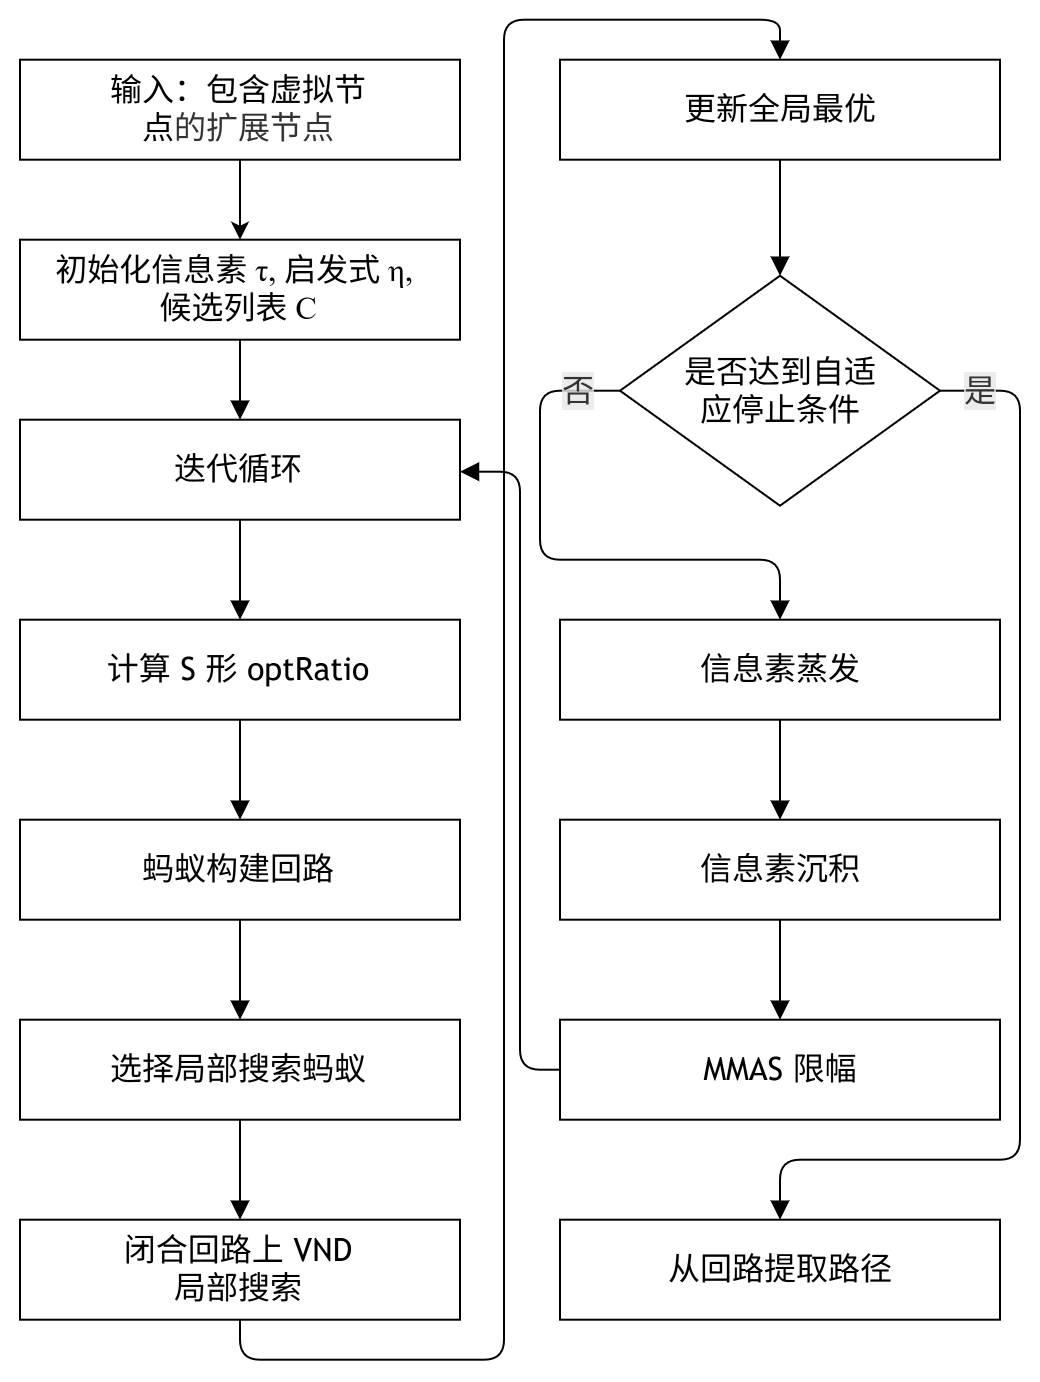
\includegraphics[width=\columnwidth]{figures/fig05_aco_flow}
\caption{改进蚁群优化总体流程图。}
\label{fig:aco_flow}
\end{figure}
\subsection{协同优化框架}
\label{subsec:coop}
前述各节分别描述了两个算法层：改进的A*规划器与路径后处理（第~\ref{subsec:jps}--\ref{subsec:post} 节），以及面向开放旅行商问题的改进蚁群优化求解器（第~\ref{subsec:aco} 节）。本节描述如何将这两个层集成为面向障碍环境多目标点遍历路径规划的统一框架。
\subsubsection{两层架构}
该框架遵循两层架构，清晰分离几何问题（障碍约束路径寻找）与组合问题（访问顺序优化）。
\textbf{第一层——代价矩阵构建。} 给定$N$个点（一个起点、$K$个目标点、一个终点），通过计算每对点之间的最短无碰撞路径构建成对代价矩阵$\mathbf{D} \in \mathbb{R}^{N \times N}$：
\begin{equation}
\mathbf{D}(i, j) = L\big(\mathrm{A}^{*}(p_i, p_j, \mathbf{M})\big) \quad \forall i \neq j \in \{1, \dots, N\}
\label{eq:dmatrix}
\end{equation}
其中$L(\cdot)$为路径长度函数，$\mathbf{M}$为占用栅格地图。对角元素为零。关键的是，$\mathbf{D}$\textbf{不是}欧氏距离矩阵：每个元素编码了真实的障碍约束最短路径距离，当障碍物阻断两点之间的直接路径时，该距离可能显著大于直线距离。
当\texttt{enableSimplify}标志激活时，路径长度$L(\cdot)$基于简化后的而非原始栅格路径计算：
\begin{equation}
\mathbf{D}_{\mathrm{simplified}}(i, j) = L_{\mathrm{Euclidean}}\big(\textsc{SimplifyPath}(\mathrm{A}^{*}(p_i, p_j, \mathbf{M}), \mathbf{M}, d_{\mathrm{safe}})\big)
\label{eq:dsimp}
\end{equation}
其中$L_{\mathrm{Euclidean}}$为简化折线的欧氏长度，其比栅格曼哈顿加对角线度量更接近真实连续路径长度。代价矩阵构建需要$O(N^2)$次全局规划器调用。可选的外部路径缓存（以起终坐标对为键的哈希映射）存储中间结果，避免在不同旅行商调用之间重复的A*计算。
\textbf{第二层——旅行商排序。} 代价矩阵$\mathbf{D}$传递给改进的蚁群优化求解器（第~\ref{subsec:aco} 节），后者纯在数值矩阵上操作。蚁群优化返回最优访问顺序$\bm{\pi}^{*} = (1, \pi_2, \dots, \pi_{K+1}, N)$及其总代价$C(\bm{\pi}^{*})$。求解器不感知障碍物、地图或路径几何——所有障碍相关信息均编码在$\mathbf{D}$中。
\subsubsection{管线集成}
集成流程按四个阶段进行：
\textbf{阶段1——点集组装。} $N = K + 2$个点组装为单一坐标数组$\mathbf{P} = [p_{\mathrm{start}};\; \mathbf{T}_1; \dots; \mathbf{T}_K;\; p_{\mathrm{goal}}]$，约定索引$1$为起点、索引$N$为终点。
\textbf{阶段2——代价矩阵构建。} 对每对有序点$(i, j)$（$i \neq j$），全局规划器计算从$\mathbf{P}(i,:)$到$\mathbf{P}(j,:)$的最短无碰撞路径。所得路径存入路径缓存，其长度根据所选代价模式赋值给$\mathbf{D}(i, j)$：
\begin{itemize}
\item 启用\texttt{enableSimplify}时，路径先经简化（第~\ref{subsec:post} 节）再取欧氏长度（式~\eqref{eq:dsimp}），产生更接近真实连续旅行距离的代价。
\item 不启用简化时，使用原始栅格路径在曼哈顿加对角线度量下的长度（式~\eqref{eq:dmatrix}）。
\end{itemize}
不可达对保留$\mathbf{D}(i, j) = \infty$。若任何目标点从起点不可达，流程提前终止并报告失败。
\textbf{阶段3——旅行商求解。} 代价矩阵$\mathbf{D}$和总点数$N$传递给改进的蚁群优化求解器（第~\ref{subsec:aco} 节），返回最优访问顺序$\mathrm{bestOrder} = (1, \dots, N)$及其总代价。在$K = 0$（无中间目标点）的平凡情况下，顺序为$[1, N]$，代价为$\mathbf{D}(1, N)$。
\textbf{阶段4——输出组装。} 有序点坐标提取为$\mathbf{P}(\mathrm{bestOrder}, :)$。对\texttt{bestOrder}中每对连续点从路径缓存检索段路径，生成最终的障碍安全参考路径集，供平滑和机器人执行使用。
\subsubsection{设计原理}
两层分离提供三个关键优势：
\textbf{1. 算法解耦。} 全局规划器和旅行商求解器可独立开发、测试和改进。任何基于栅格的规划器（A*、Dijkstra、RRT）可替换到第一层，任何排列优化器（蚁群优化、遗传算法、模拟退火）可替换到第二层。此模块化在实验（第~\ref{subsec:exp_sens}--\ref{subsec:exp_cmp} 节）中得到验证——每层针对替代实现进行基准测试，同时另一层保持固定。
\textbf{2. 通过代价矩阵编码障碍信息。} 代价矩阵$\mathbf{D}$作为紧凑接口：无论地图复杂度如何，它将完整的障碍约束距离拓扑捕获在$N \times N$矩阵中。旅行商求解器免费继承障碍感知——它从不直接查询占用栅格，但每对点都保证有无碰撞路径（若存在）。此编码在旅行商求解器无法推理路径几何（例如两段路径是否共享走廊）的意义上是有损的，但对于代价最小化目的是完备的。
\textbf{3. 通过简化提升代价精度。} \texttt{enableSimplify}标志控制一个关键的设计权衡。禁用时，代价基于原始栅格路径在栅格度量下计算（正交边代价1，对角边代价$\sqrt{2}$），因阶梯伪影而高估真实连续路径长度。启用时，路径先经简化（通过第~\ref{subsec:post} 节去除锯齿航点）再以简化折线的欧氏长度计算代价。这产生更接近物理旅行距离的代价矩阵，以每对点对调用\textsc{SimplifyPath}的适度额外计算代价为代价。
\subsubsection{完整系统流程}
端到端系统按以下步骤运行：
\begin{enumerate}
\item \textbf{构建代价矩阵}：对所有$O(N^2)$个点对调用改进的A*规划器，可选地在代价评估前简化路径。
\item \textbf{求解开放旅行商问题}：使用改进的蚁群优化确定最优访问顺序。
\item \textbf{检索段路径}：从路径缓存中组装完整有序轨迹。
\item \textbf{应用后处理管线}：对每段路径应用SimplifyPath + SmoothPath（第~\ref{subsec:post} 节），生成供机器人执行使用的平滑、障碍安全的连续轨迹。系统架构总图如图~\ref{fig:system}所示。
\end{enumerate}
\begin{figure}[!t]
\centering
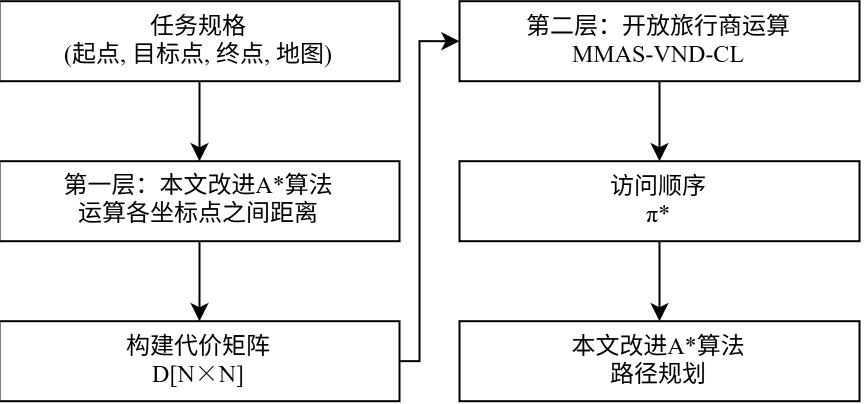
\includegraphics[width=\columnwidth]{figures/fig06_system}
\caption{系统架构总图}
\label{fig:system}
\end{figure}

\section{实验}

\label{sec:exp}

本节对所提框架进行全面的实验评估。我们进行四组实验：（1）改进的A*全局规划器（基于JPS）与基线规划器的性能对比；（2）改进蚁群优化求解器的参数敏感性分析；（3）隔离蚁群优化各组件贡献的消融实验；（4）不同旅行商求解器与改进A*规划器协同完成多目标点遍历的对比实验。

\subsection{实验设置}

所有实验在配备Intel Core Ultra 5 125H处理器和16~GB内存的计算机上进行，运行MATLAB R2025b。

\textbf{测试地图。} 两张栅格地图（Map~1和Map~2）为所有实验共用。第三张地图在两组实验之间不同：全局路径规划对比（第~\ref{subsec:exp_plan} 节）使用$80\times 80$迷宫栅格地图，而旅行商实验（第~\ref{subsec:exp_sens}--\ref{subsec:exp_cmp} 节）使用kroB100 TSPLIB基准数据集。

\begin{itemize}

\item \textbf{Map~1}（\texttt{Map1.mat}）：一个中等障碍密度的栅格地图，用于测试基本搜索性能（所有实验共用）。

\item \textbf{Map~2}（\texttt{Map2\_kong.mat}）：一个更大的栅格地图，具有开阔、走廊式的结构，考验长距离直线遍历，并在栅格路径中产生显著的阶梯伪影（所有实验共用）。

\item \textbf{Map~3}（\texttt{迷宫x80\_3.mat}）：一个$80\times 80$迷宫栅格地图，仅用于全局路径规划对比（第~\ref{subsec:exp_plan} 节）。

\item \textbf{kroB100}（\texttt{kroB100\_coords.mat}）：一个标准的100城市TSPLIB基准实例，仅用于旅行商排序实验（第~\ref{subsec:exp_sens}--\ref{subsec:exp_cmp} 节）。

\end{itemize}

\textbf{重复次数与统计。} 全局路径规划对比（第~\ref{subsec:exp_plan} 节）中，每个算法在每张地图上运行10次，时间指标取平均。旅行商实验（第~\ref{subsec:exp_sens}--\ref{subsec:exp_cmp} 节）中，每个算法配置在每张地图上运行40次，统计指标（最优值、中位数、均值、标准差、成功率和代价极差）基于40次独立运行计算。

\textbf{参数设置。} 除非在敏感性分析（第~\ref{subsec:exp_sens} 节）或消融实验（第~\ref{subsec:exp_ablation} 节）中另有说明，全文使用表~\ref{tab:params}中的默认参数值。

\begin{table}[!t]

\caption{所提算法的默认参数设置}
\label{tab:params}
\centering
\begin{tabular}{lll}
\toprule
模块 & 参数 & 值 \\
\midrule
A* (JPS) & 回退规划器 & AStar\_v0 \\
A* (JPS) & 启发式 & 标准欧氏距离 \\
路径简化 & 安全距离$d_{\mathrm{safe}}$ & 0.4 \\
路径平滑 & 插值密度$\rho$ & 10 \\
蚁群优化 & 蚂蚁数量$n_{\mathrm{ants}}$ & 40 \\
蚁群优化 & 信息素权重$\alpha$ & 1 \\
蚁群优化 & 启发式权重$\beta$ & 2.0 \\
蚁群优化 & 蒸发率$\rho_{\mathrm{ACO}}$ & 0.25 \\
蚁群优化 & 沉积常数$Q$ & 225 \\
蚁群优化 & 初始信息素$\tau_0$ & 0.1 \\
蚁群优化 & 贪心概率$q_0$ & 0.45 \\
蚁群优化 & 局部搜索比例$y_{\max}$ & 0.4 \\
蚁群优化 & 局部搜索转换区间$[x_L, x_R]$ & $[0, 30]$ \\
蚁群优化 & 精英比率$r_{\mathrm{elite}}$ & 0.7 \\
蚁群优化 & 候选列表大小$k$ & 9 \\
\bottomrule
\end{tabular}
\end{table}
\textbf{评估指标。} 报告以下指标：路径长度（栅格单位）、计算时间（秒）、扩展节点数（仅限全局规划）、最优/中位/平均收敛代价、成功率（达到最优代价的运行百分比）和标准差。
\subsection{全局路径规划对比}
\label{subsec:exp_plan}
\textbf{目标。} 对比所提基于JPS的A*规划器（AStar\_v3\_1，结合SimplifyPath和SmoothPath）与三个基线规划器的搜索效率和路径质量：传统A*（AStar\_v0）、Dijkstra和RRT。
\textbf{流程。} 每个规划器在三张栅格地图（Map~1、Map~2和Map~3，即$80\times 80$迷宫）上运行。对于所提方法，报告结果包含完整后处理管线（SimplifyPath + SmoothPath）。每个算法在每张地图上运行10次，计算时间取平均。
\textbf{结果。} 表~\ref{tab:plan}汇总了每个算法在每张地图上的路径长度、计算时间和扩展节点数。RRT是基于采样的方法，因此不报告扩展节点数。路径规划可视化结果见图~\ref{fig:plan_paths}。
\begin{table}[!t]
\caption{全局路径规划性能对比}
\label{tab:plan}
\centering
\footnotesize
\begin{tabular}{llccc}
\toprule
算法 & 地图 & 路径长度 & 时间 (ms) & 扩展节点数 \\
\midrule
\multirow{3}{*}{AStar\_v3\_1+后处理（本文）}
& Map 1 & 72.93 & 2.45 & 70 \\
& Map 2 & 108.17 & 11.85 & 415 \\
& Map 3 & 113.33 & 4.31 & 48 \\
\midrule
\multirow{3}{*}{AStar\_v0}
& Map 1 & 76.53 & 6.14 & 81 \\
& Map 2 & 111.44 & 29.19 & 198 \\
& Map 3 & 119.64 & 17.88 & 280 \\
\midrule
\multirow{3}{*}{Dijkstra}
& Map 1 & 76.53 & 24.26 & 200 \\
& Map 2 & 111.44 & 202.29 & 522 \\
& Map 3 & 119.64 & 204.46 & 566 \\
\midrule
\multirow{3}{*}{RRT}
& Map 1 & 100.80 & 7.42 & --- \\
& Map 2 & 135.40 & 19.33 & --- \\
& Map 3 & 144.07 & 3.69 & --- \\
\bottomrule
\end{tabular}
\end{table}
\textbf{分析。} 所提基于JPS的规划器在所有三张地图上均取得最短路径长度（Map~1上72.93对比AStar\_v0和Dijkstra的76.53；Map~2上108.17对比111.44；Map~3上113.33对比119.64）。此路径长度优势源于简化阶段，其去除了阶梯伪影并有效缩短路径。在搜索效率方面，JPS规划器比基线方法扩展更少的节点：Map~3上仅扩展48个节点，对比AStar\_v0的280个和Dijkstra的566个，减少超过80\%。这直接转化为更快的计算速度：Map~2上所提方法以11.85~ms完成，对比AStar\_v0的29.19~ms和Dijkstra的202.29~ms——比Dijkstra快17倍以上。RRT产生最长路径（Map~1上100.80、Map~2上135.40、Map~3上144.07），方差较高，与其基于采样的性质一致。结果表明，JPS剪枝、路径简化和平滑的组合相比基线方法产生了更短且计算效率更高的路径。路径可视化对比如图~\ref{fig:plan_paths}所示，路径长度与计算时间对比分别如图~\ref{fig:plan_len}和图~\ref{fig:plan_time}所示。
\begin{figure*}[!t]
\centering
\subfloat[本文A*（JPS）规划器]{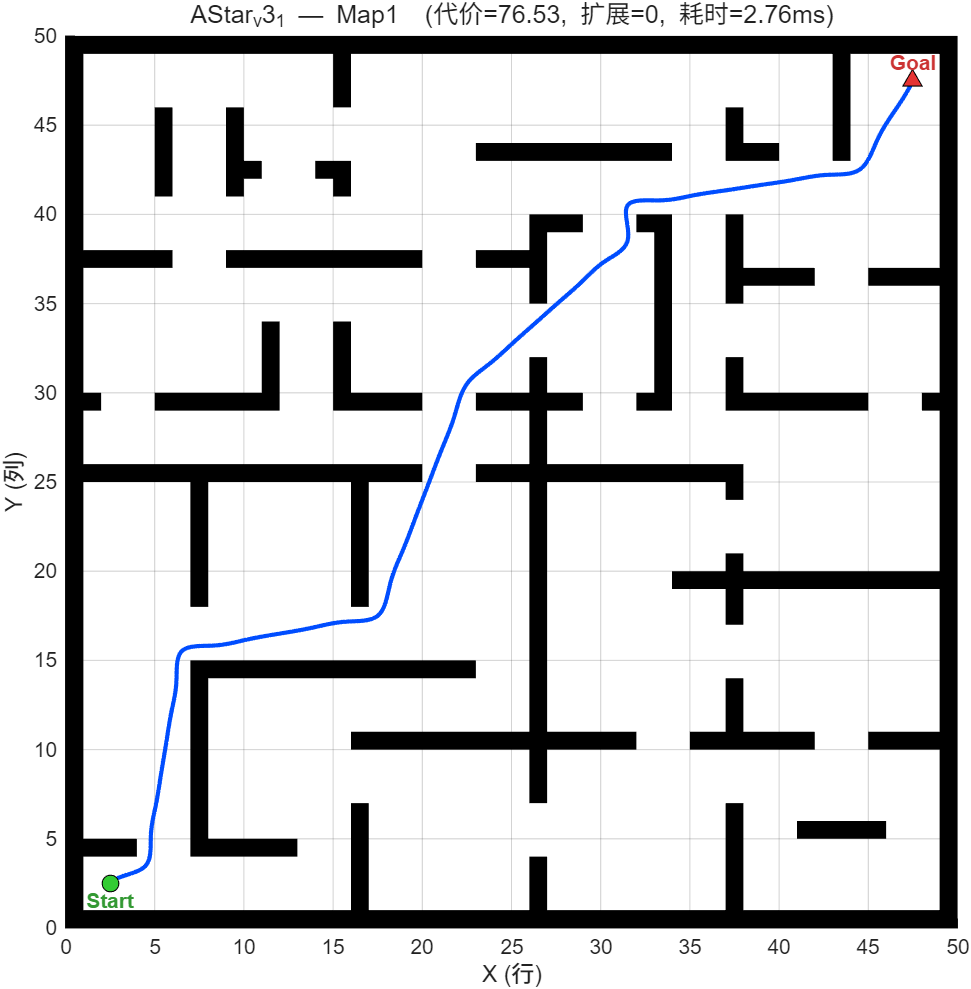
\includegraphics[width=0.22\textwidth]{figures/fig07a_jps_m1}\hfil
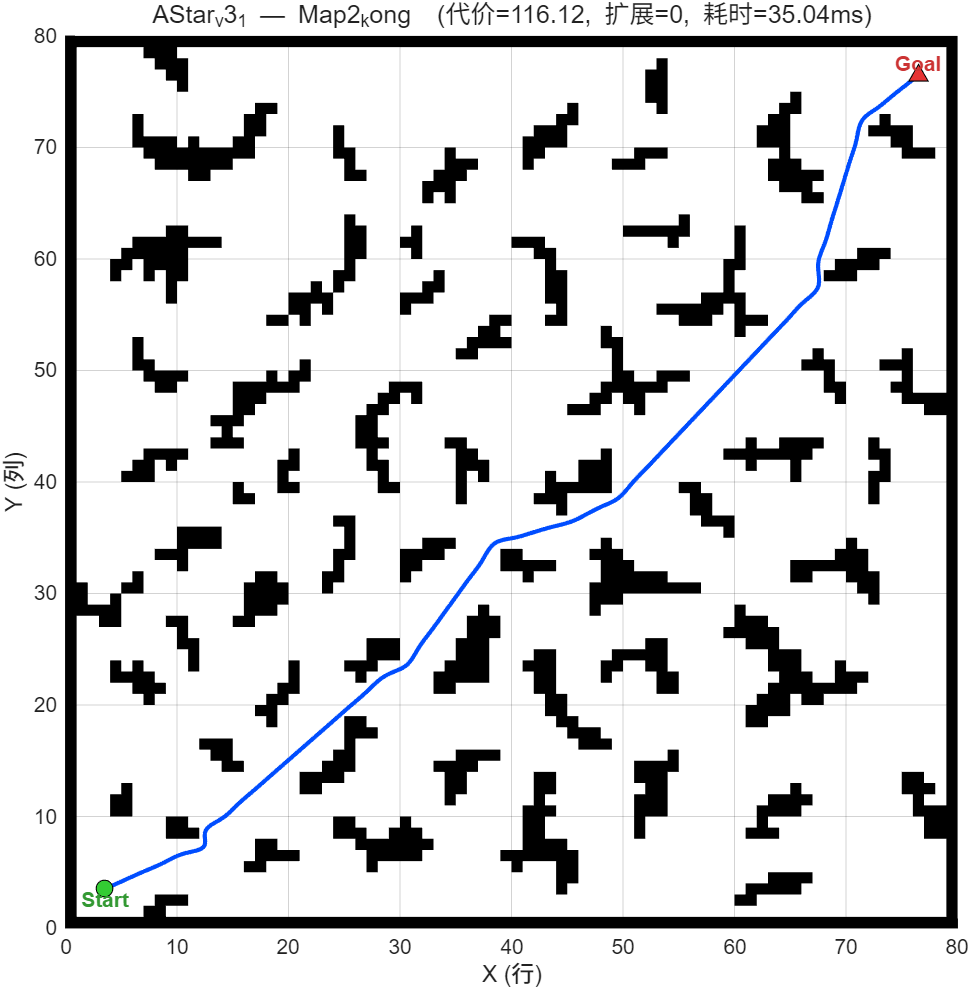
\includegraphics[width=0.22\textwidth]{figures/fig07a_jps_m2}\hfil
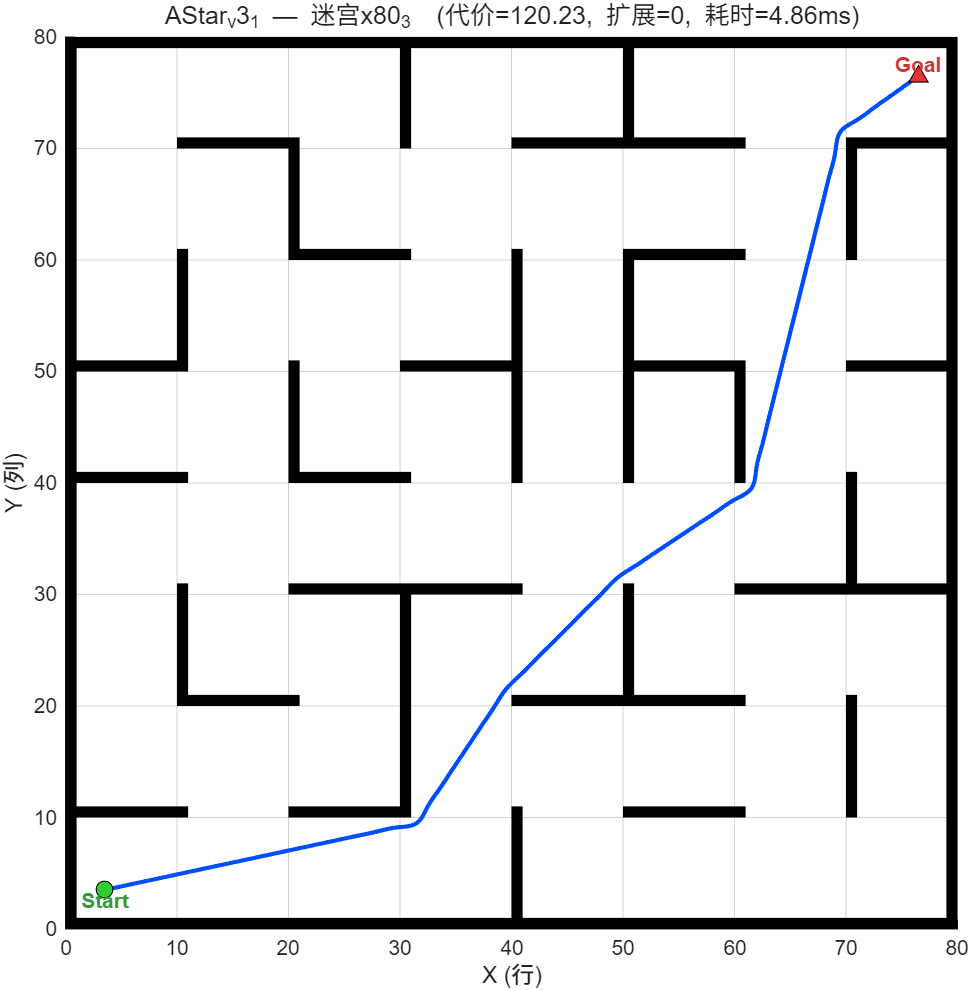
\includegraphics[width=0.22\textwidth]{figures/fig07a_jps_m3}}\\
\subfloat[传统A*]{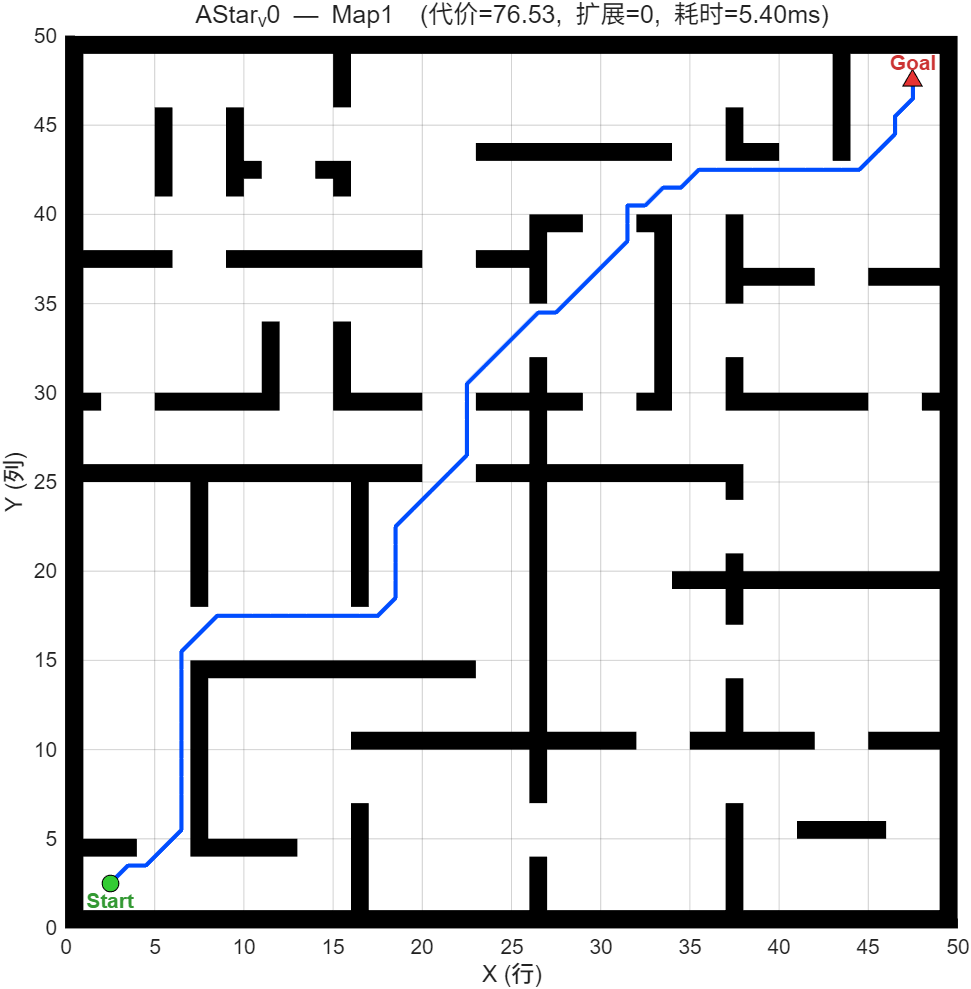
\includegraphics[width=0.22\textwidth]{figures/fig07b_astar_m1}\hfil
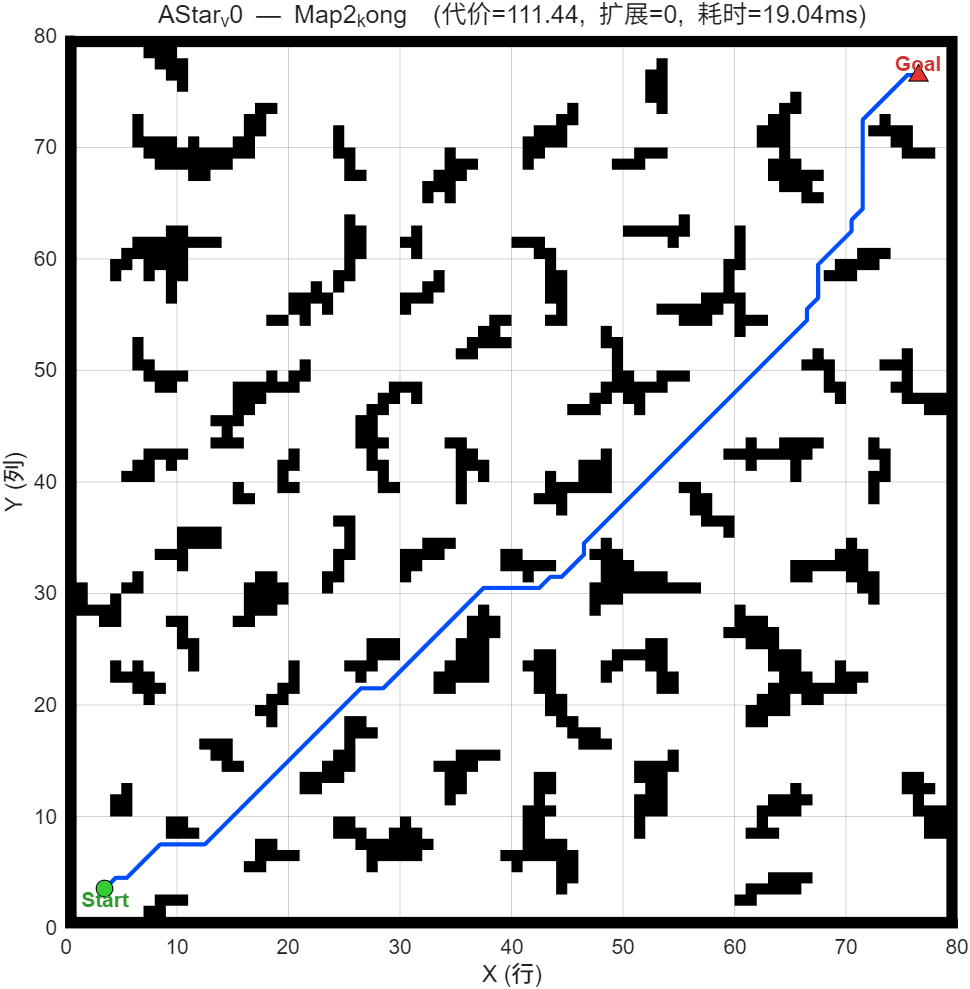
\includegraphics[width=0.22\textwidth]{figures/fig07b_astar_m2}\hfil
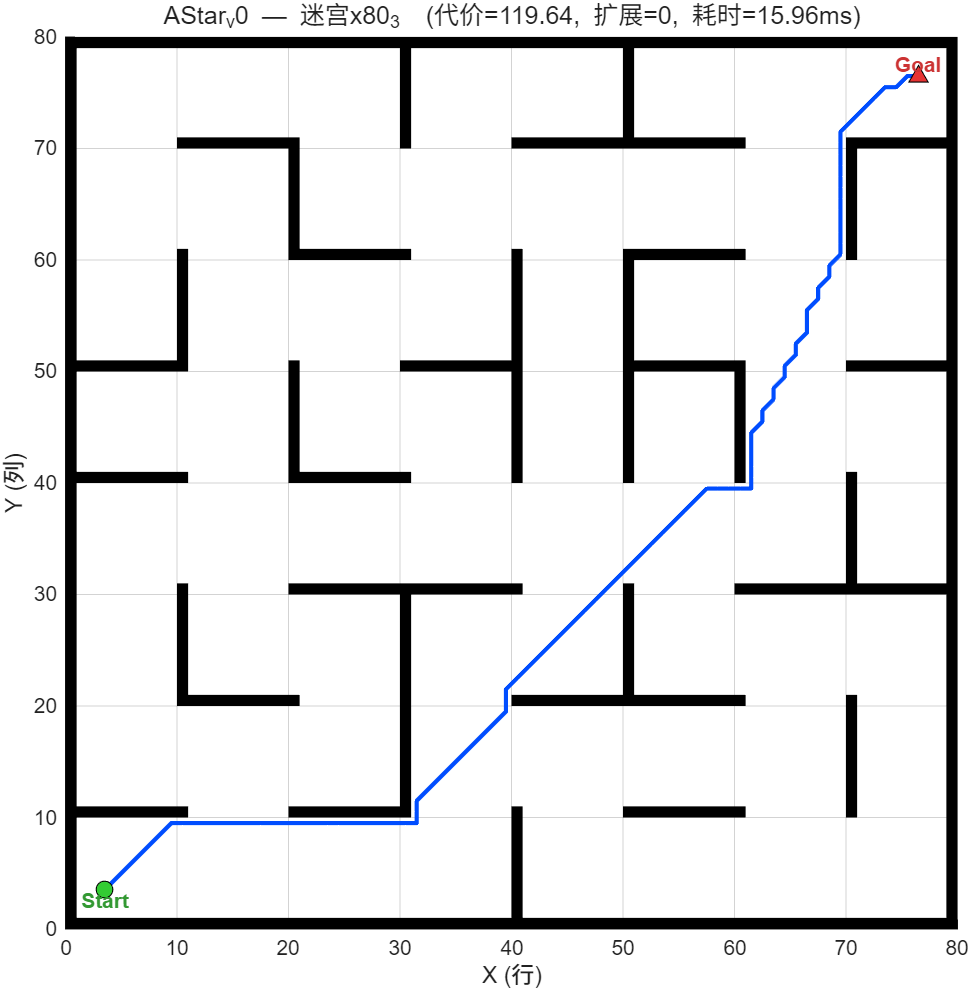
\includegraphics[width=0.22\textwidth]{figures/fig07b_astar_m3}}\\
\subfloat[Dijkstra]{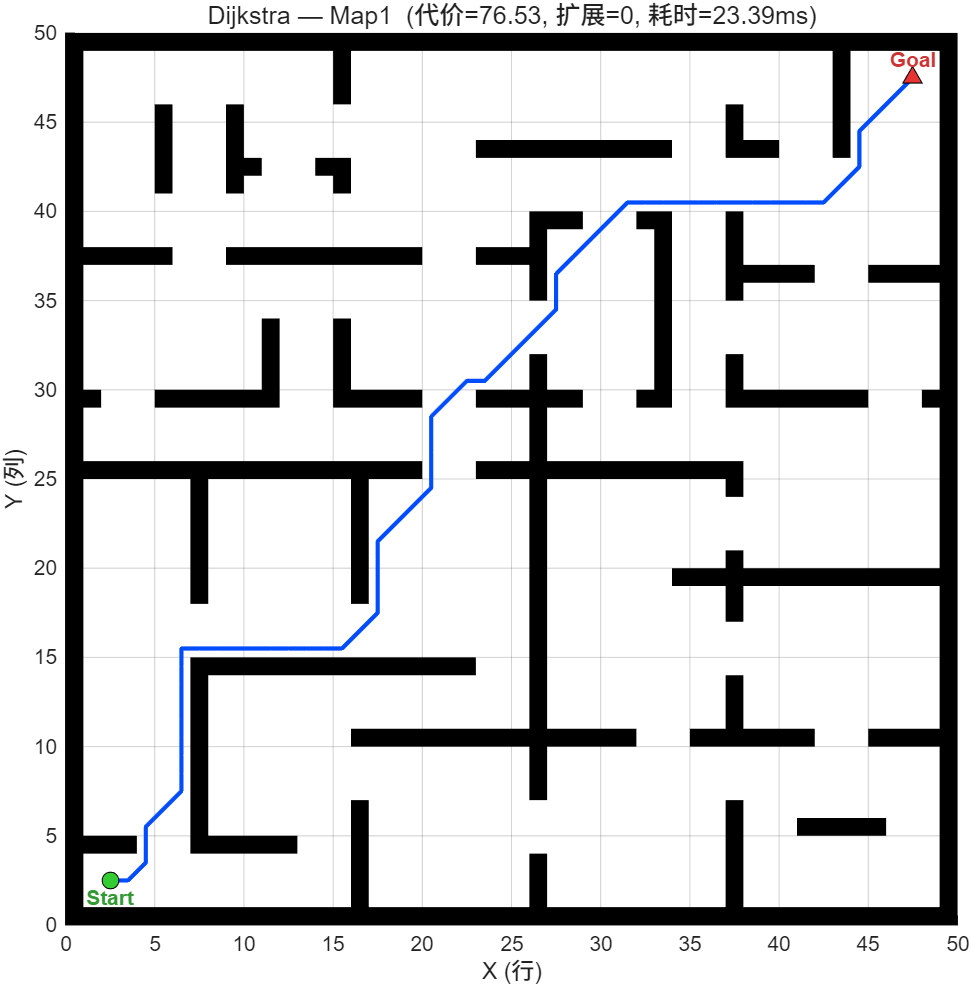
\includegraphics[width=0.22\textwidth]{figures/fig07c_dijk_m1}\hfil
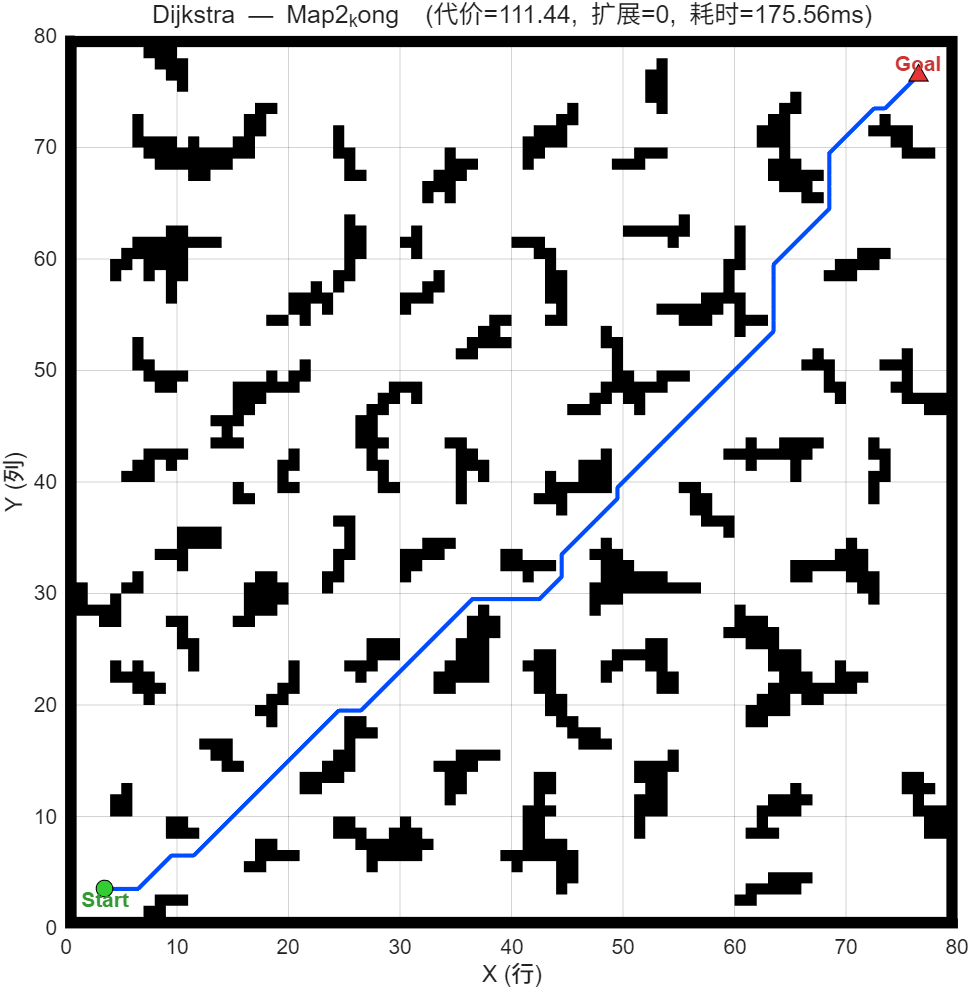
\includegraphics[width=0.22\textwidth]{figures/fig07c_dijk_m2}\hfil
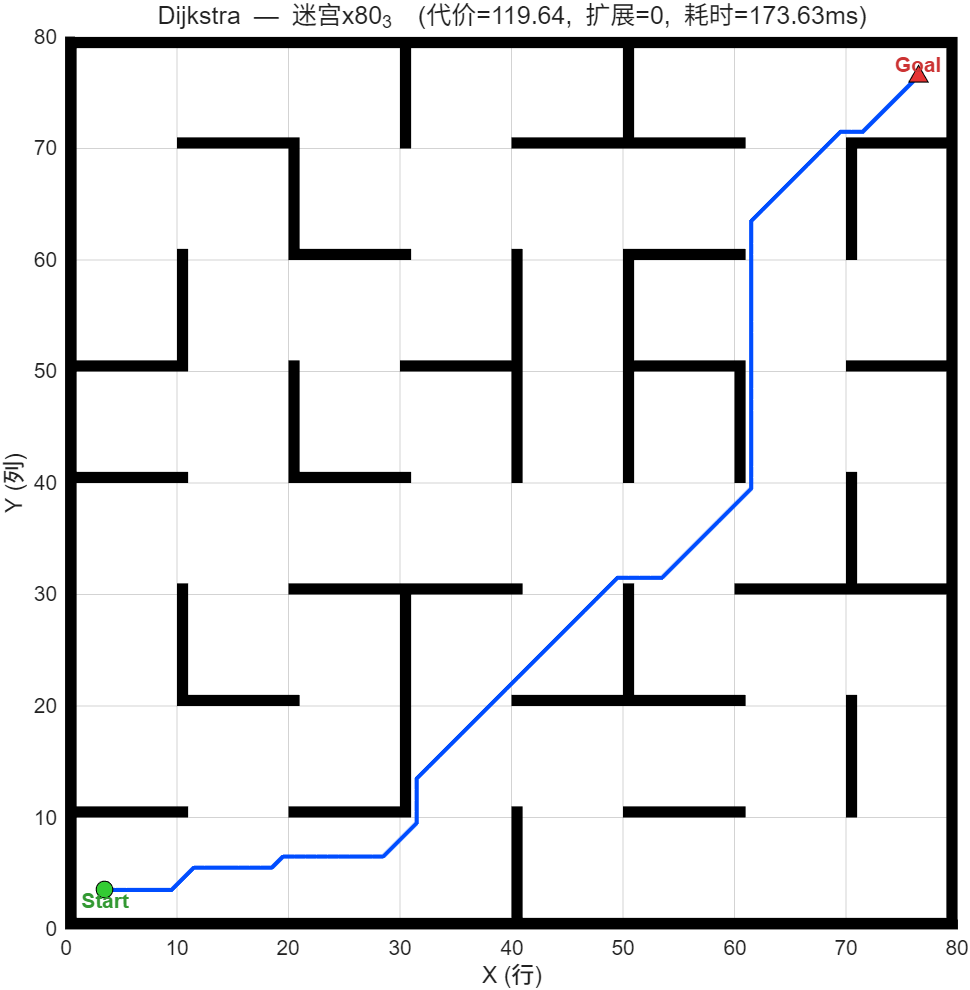
\includegraphics[width=0.22\textwidth]{figures/fig07c_dijk_m3}}\\
\subfloat[RRT]{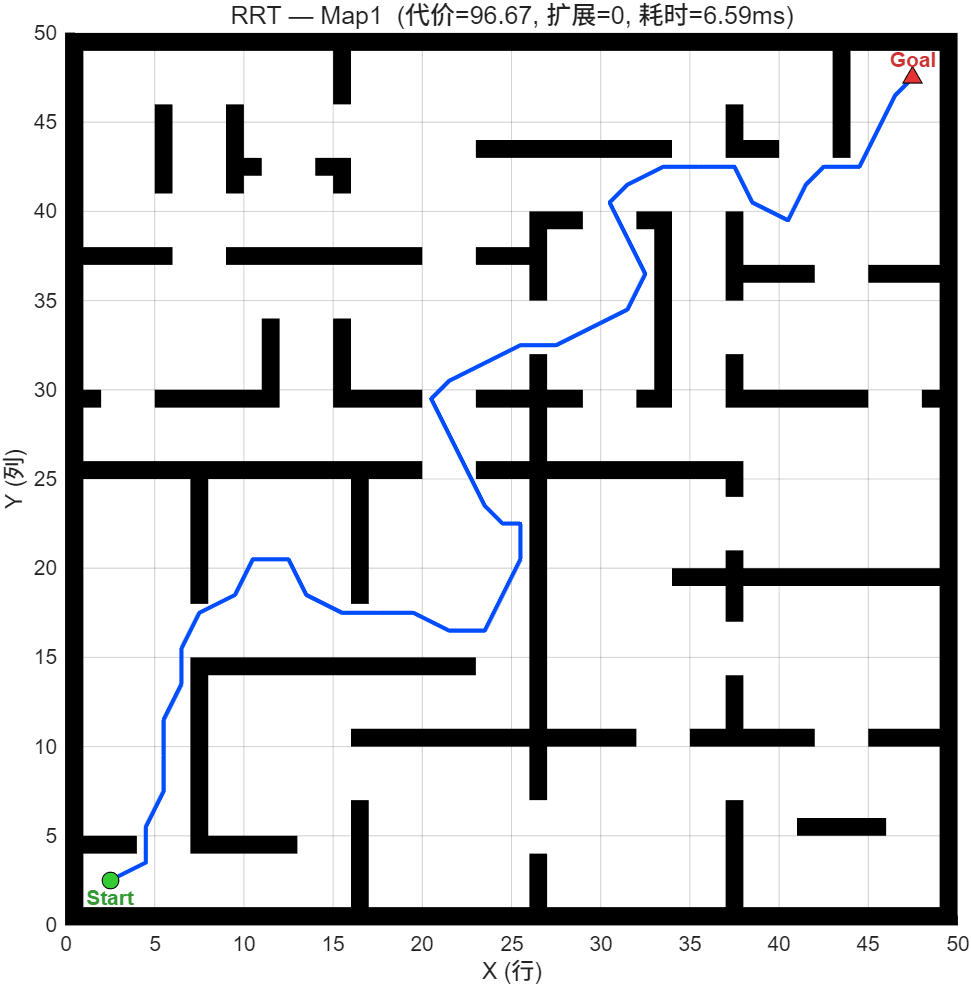
\includegraphics[width=0.22\textwidth]{figures/fig07d_rrt_m1}\hfil
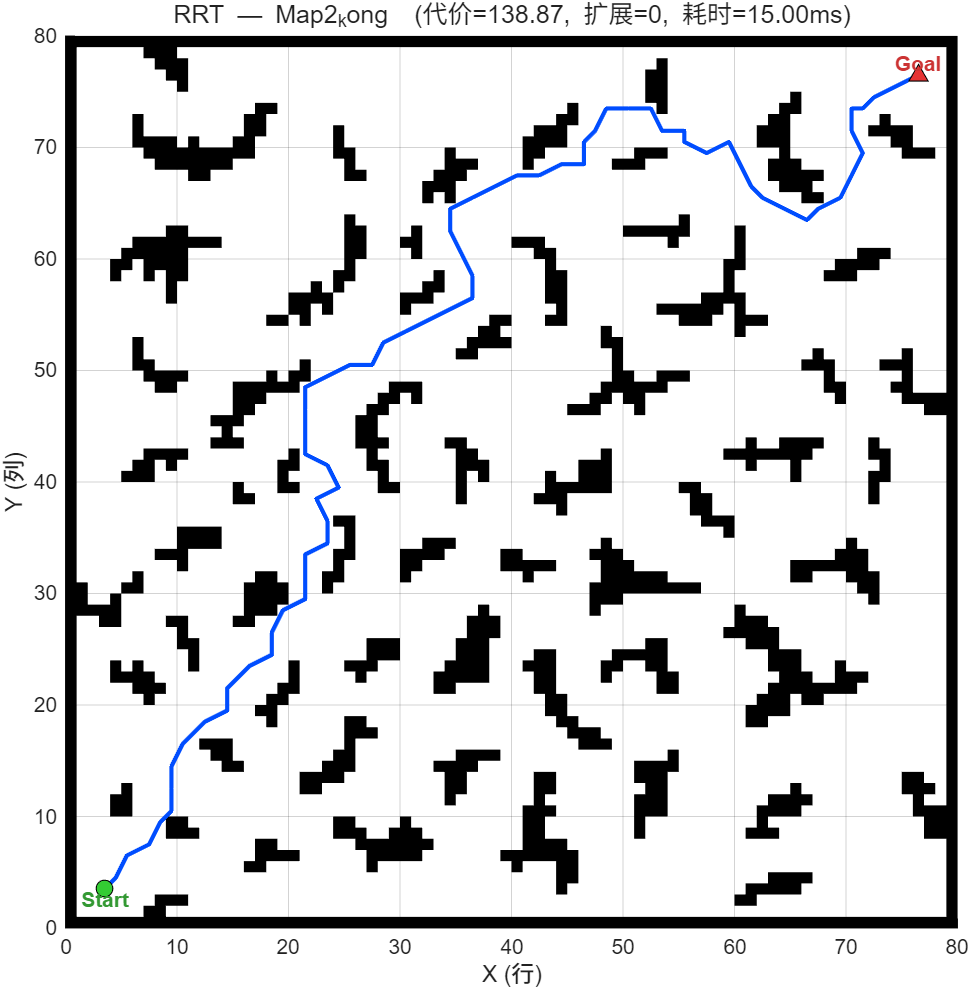
\includegraphics[width=0.22\textwidth]{figures/fig07d_rrt_m2}\hfil
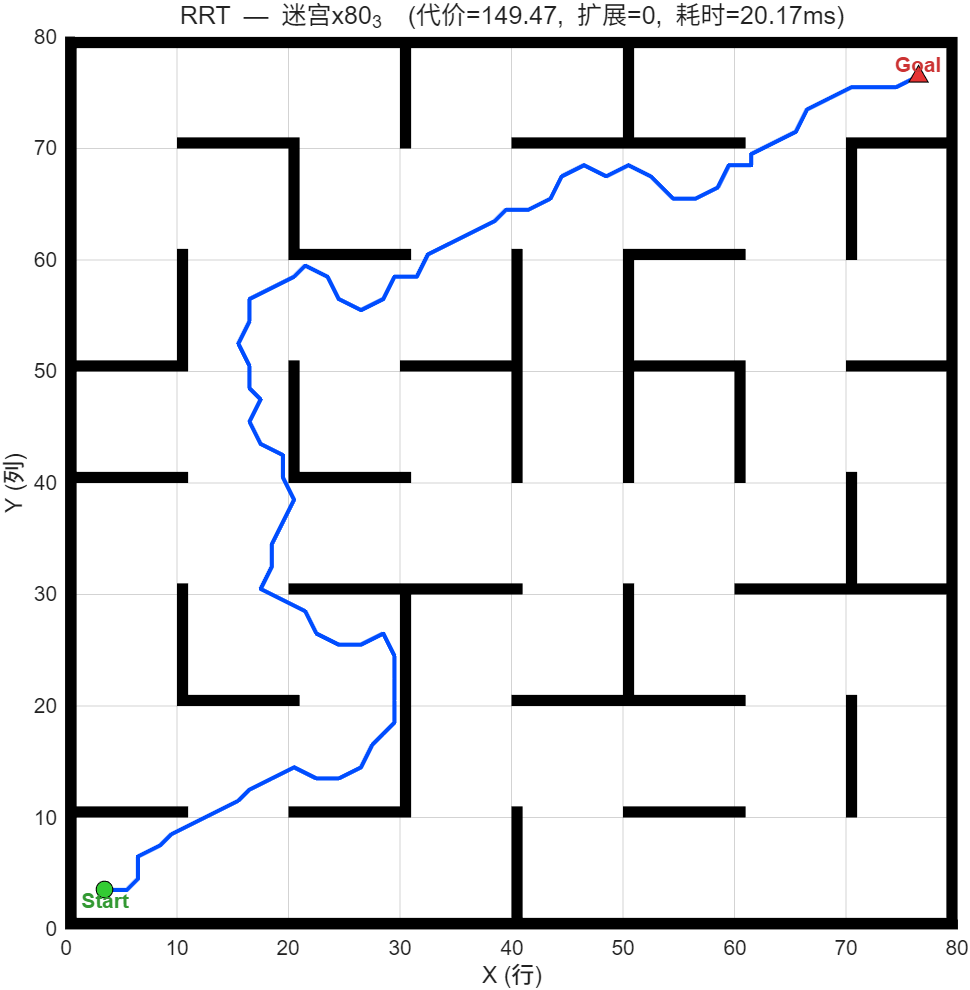
\includegraphics[width=0.22\textwidth]{figures/fig07d_rrt_m3}}
\caption{四种算法在三张地图上的路径规划结果。每行从左至右依次为Map~1、Map~2、Map~3。}
\label{fig:plan_paths}
\end{figure*}
\begin{figure}[!t]
\centering
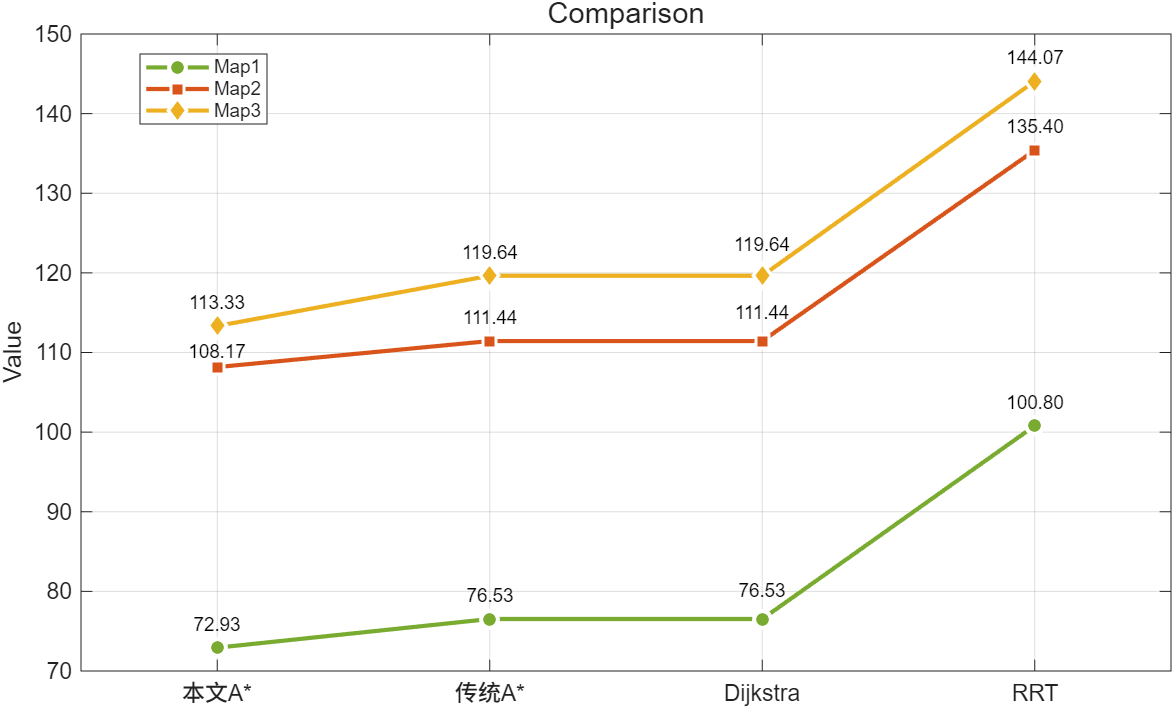
\includegraphics[width=2.5in]{figures/fig08_pathlen}
\caption{四个算法在Map~1、2、3上的路径长度对比（折线图）。}
\label{fig:plan_len}
\end{figure}
\begin{figure}[!t]
\centering
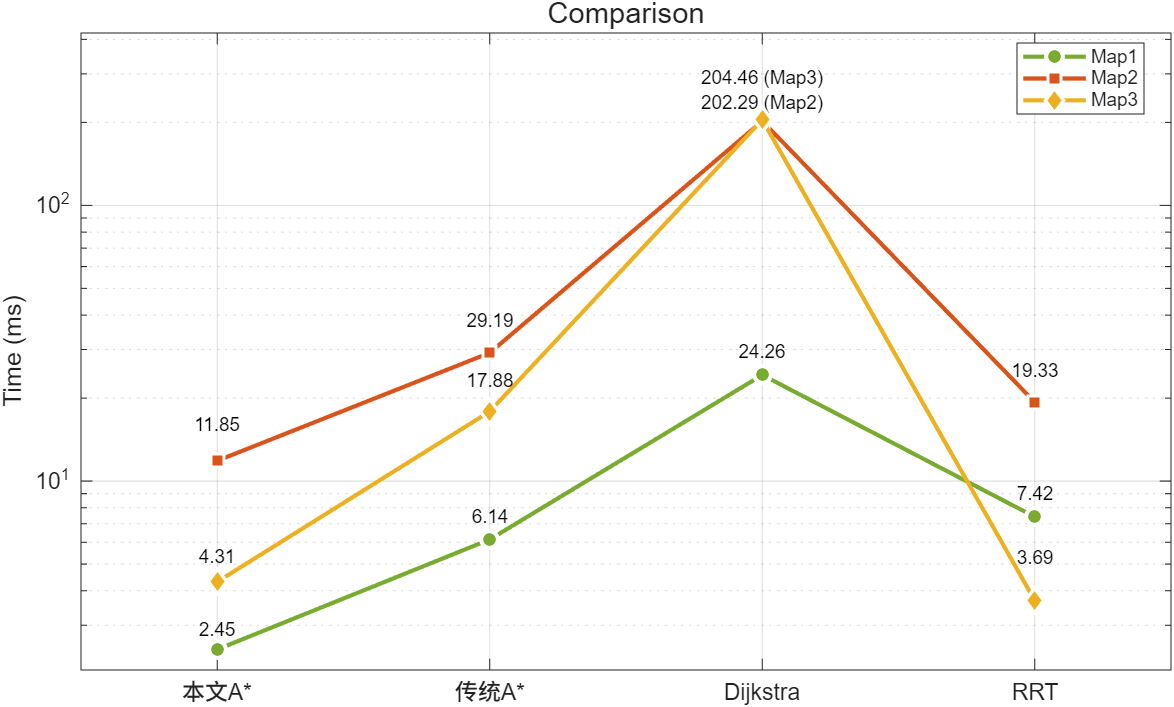
\includegraphics[width=2.5in]{figures/fig09_time}
\caption{四个算法在Map~1、2、3上的计算时间对比（折线图）。}
\label{fig:plan_time}
\end{figure}
\subsection{参数敏感性分析}
\label{subsec:exp_sens}
\textbf{目标。} 分析改进蚁群优化求解器（TSP\_ACO\_v2\_4）对五个关键超参数的敏感性：蚂蚁数量$n_{\mathrm{ants}}$、贪心选择概率$q_0$、后期局部搜索比例$y_{\max}$（optRatio\_end）、精英比率$r_{\mathrm{elite}}$（optEliteRatio）和候选列表大小$k$（kCand）。
\textbf{流程。} 每个参数在五个水平上变化，同时其他参数保持默认值。每个参数的五个水平汇总于表~\ref{tab:levels}。每个配置在每张地图上运行40次。
\begin{table}[!t]
\caption{敏感性分析中使用的参数水平}
\label{tab:levels}
\centering
\begin{tabular}{lccccc}
\toprule
参数 & 水平1 & 水平2 & 水平3（默认） & 水平4 & 水平5 \\
\midrule
$n_{\mathrm{ants}}$ & 10 & 20 & 40 & 60 & 90 \\
$q_0$ & 0.10 & 0.30 & 0.45 & 0.60 & 0.90 \\
$y_{\max}$ & 0.10 & 0.20 & 0.40 & 0.60 & 0.90 \\
$r_{\mathrm{elite}}$ & 0.1 & 0.3 & 0.5 & 0.7 & 0.9 \\
$k$ & 3 & 9 & 15 & 30 & 60 \\
\bottomrule
\end{tabular}
\end{table}
\textbf{结果。} 表~\ref{tab:sens}展示了完整敏感性结果（25种配置$\times$3张地图）。参数水平依次为$n_{\mathrm{ants}}/q_0/y_{\max}/r_{\mathrm{elite}}/k$。
\begin{table}[!t]
\caption{代表性参数敏感性结果}
\label{tab:sens}
\centering
\scriptsize
\setlength{\tabcolsep}{2pt}
\resizebox{\columnwidth}{!}{%
\begin{tabular}{llccccc}
\toprule
取值等级 & 地图 & 最优代价 & 平均收敛代价 & 成功率(\%) & 平均时间(ms) & 标准差 \\
\midrule
1/3/3/4/2 & Map~1 & 351.44 & 351.44 & 100 & 9.1 & 0 \\
1/3/3/4/2 & Map~2 & 620.15 & 620.34 & 80 & 148.0 & 0.44 \\
1/3/3/4/2 & kroB100 & 22141.00 & 22145.03 & 92.5 & 250.5 & 14.66 \\
2/3/3/4/2 & Map~1 & 351.44 & 351.44 & 100 & 15.1 & 0 \\
2/3/3/4/2 & Map~2 & 620.15 & 620.27 & 85 & 204.7 & 0.29 \\
2/3/3/4/2 & kroB100 & 22141.00 & 22143.90 & 95 & 254.8 & 12.80 \\
3/3/3/4/2 & Map~1 & 351.44 & 351.44 & 100 & 27.2 & 0 \\
3/3/3/4/2 & Map~2 & 620.15 & 620.15 & 100 & 241.5 & 0 \\
3/3/3/4/2 & kroB100 & 22141.00 & 22142.45 & 97.5 & 347.9 & 9.17 \\
4/3/3/4/2 & Map~1 & 351.44 & 351.44 & 100 & 40.4 & 0 \\
4/3/3/4/2 & Map~2 & 620.15 & 620.15 & 100 & 371.1 & 0 \\
4/3/3/4/2 & kroB100 & 22141.00 & 22141.00 & 100 & 480.5 & 0 \\
5/3/3/4/2 & Map~1 & 351.44 & 351.44 & 100 & 52.7 & 0 \\
5/3/3/4/2 & Map~2 & 620.15 & 620.15 & 100 & 336.3 & 0 \\
5/3/3/4/2 & kroB100 & 22141.00 & 22142.45 & 97.5 & 628.7 & 9.17 \\
3/1/3/4/2 & Map~1 & 351.44 & 351.44 & 100 & 37.8 & 0 \\
3/1/3/4/2 & Map~2 & 620.15 & 620.17 & 97.5 & 426.5 & 0.13 \\
3/1/3/4/2 & kroB100 & 22141.00 & 22141.00 & 100 & 548.4 & 0 \\
3/2/3/4/2 & Map~1 & 351.44 & 351.44 & 100 & 27.2 & 0 \\
3/2/3/4/2 & Map~2 & 620.15 & 620.15 & 100 & 311.8 & 0 \\
3/2/3/4/2 & kroB100 & 22141.00 & 22141.00 & 100 & 475.7 & 0 \\
3/4/3/4/2 & Map~1 & 351.44 & 351.44 & 100 & 30.5 & 0 \\
3/4/3/4/2 & Map~2 & 620.15 & 620.19 & 95 & 257.0 & 0.18 \\
3/4/3/4/2 & kroB100 & 22141.00 & 22143.90 & 95 & 296.7 & 12.80 \\
3/5/3/4/2 & Map~1 & 351.44 & 351.44 & 100 & 38.5 & 0 \\
3/5/3/4/2 & Map~2 & 620.15 & 620.75 & 62.5 & 232.1 & 1.17 \\
3/5/3/4/2 & kroB100 & 22141.00 & 22180.55 & 50 & 351.7 & 42.06 \\
3/3/1/4/2 & Map~1 & 351.44 & 351.44 & 100 & 44.4 & 0 \\
3/3/1/4/2 & Map~2 & 620.15 & 620.71 & 65 & 217.1 & 1.05 \\
3/3/1/4/2 & kroB100 & 22141.00 & 22157.05 & 80 & 365.4 & 35.39 \\
3/3/2/4/2 & Map~1 & 351.44 & 351.44 & 100 & 32.2 & 0 \\
3/3/2/4/2 & Map~2 & 620.15 & 620.35 & 75 & 247.2 & 0.35 \\
3/3/2/4/2 & kroB100 & 22141.00 & 22143.40 & 95 & 294.5 & 10.83 \\
3/3/4/4/2 & Map~1 & 351.44 & 351.44 & 100 & 24.9 & 0 \\
3/3/4/4/2 & Map~2 & 620.15 & 620.15 & 100 & 309.0 & 0 \\
3/3/4/4/2 & kroB100 & 22141.00 & 22142.45 & 97.5 & 350.1 & 9.17 \\
3/3/5/4/2 & Map~1 & 351.44 & 351.44 & 100 & 28.1 & 0 \\
3/3/5/4/2 & Map~2 & 620.15 & 620.15 & 100 & 356.3 & 0 \\
3/3/5/4/2 & kroB100 & 22141.00 & 22141.00 & 100 & 407.1 & 0 \\
3/3/3/1/2 & Map~1 & 351.44 & 351.44 & 100 & 32.1 & 0 \\
3/3/3/1/2 & Map~2 & 620.15 & 620.15 & 100 & 355.5 & 0 \\
3/3/3/1/2 & kroB100 & 22141.00 & 22141.00 & 100 & 474.8 & 0 \\
3/3/3/2/2 & Map~1 & 351.44 & 351.44 & 100 & 40.0 & 0 \\
3/3/3/2/2 & Map~2 & 620.15 & 620.17 & 97.5 & 344.4 & 0.13 \\
3/3/3/2/2 & kroB100 & 22141.00 & 22141.00 & 100 & 421.5 & 0 \\
3/3/3/3/2 & Map~1 & 351.44 & 351.44 & 100 & 27.5 & 0 \\
3/3/3/3/2 & Map~2 & 620.15 & 620.15 & 100 & 272.8 & 0 \\
3/3/3/3/2 & kroB100 & 22141.00 & 22142.45 & 97.5 & 357.8 & 9.17 \\
3/3/3/5/2 & Map~1 & 351.44 & 351.44 & 100 & 21.7 & 0.02 \\
3/3/3/5/2 & Map~2 & 620.15 & 620.21 & 92.5 & 211.6 & 0.22 \\
3/3/3/5/2 & kroB100 & 22141.00 & 22145.35 & 92.5 & 342.0 & 15.47 \\
3/3/3/4/1 & Map~1 & 351.44 & 351.44 & 100 & 37.8 & 0 \\
3/3/3/4/1 & Map~2 & 620.15 & 620.17 & 97.5 & 217.8 & 0.13 \\
3/3/3/4/1 & kroB100 & 22141.00 & 22193.30 & 30 & 786.8 & 37.45 \\
3/3/3/4/3 & Map~1 & 351.44 & 351.44 & 100 & 33.8 & 0 \\
3/3/3/4/3 & Map~2 & 620.15 & 620.15 & 100 & 243.2 & 0 \\
3/3/3/4/3 & kroB100 & 22141.00 & 22143.90 & 95 & 404.3 & 12.80 \\
3/3/3/4/4 & Map~1 & 351.44 & 351.44 & 100 & 33.5 & 0 \\
3/3/3/4/4 & Map~2 & 620.15 & 620.17 & 97.5 & 286.0 & 0.13 \\
3/3/3/4/4 & kroB100 & 22141.00 & 22142.45 & 97.5 & 390.8 & 9.17 \\
3/3/3/4/5 & Map~1 & 351.44 & 351.44 & 100 & 28.3 & 0 \\
3/3/3/4/5 & Map~2 & 620.15 & 620.19 & 95 & 287.7 & 0.18 \\
3/3/3/4/5 & kroB100 & 22141.00 & 22142.45 & 97.5 & 487.7 & 9.17 \\
\bottomrule
\end{tabular}
}
\end{table}

\textbf{分析。} 结果揭示了若干重要的敏感性特征。首先，蚂蚁数量$n_{\mathrm{ants}}$具有中等影响：在$n_{\mathrm{ants}} = 40$（默认值）时，算法在Map~2上达到100\%成功率、kroB100上达97.5\%，而减至10只蚂蚁使kroB100成功率降至92.5\%并增加平均代价。其次，贪心概率$q_0$在默认值0.45处呈现明确最优：增至0.9（近纯贪心）导致严重退化，kroB100成功率降至50\%、标准差增至42.06，表明过早收敛。第三，后期局部搜索比例$y_{\max}$至关重要：减至0.10使Map~2成功率降至65\%、kroB100降至80\%，证实密集后期局部搜索对解质量不可或缺。第四，精英比率$r_{\mathrm{elite}}$和候选列表大小$k$的敏感性相对温和，候选列表大小$k$是最不敏感的参数——但过小的$k = 3$使kroB100成功率降至30\%，表明最小候选列表对有效VND剪枝是必要的。总体而言，默认参数设置代表均衡配置，因此被用于所有后续实验。各参数水平的代价与时间对比如图~\ref{fig:sens_cost}和图~\ref{fig:sens_time}所示，默认参数下规划路径如图~\ref{fig:sens_paths}所示。

\begin{figure*}[!t]

\centering
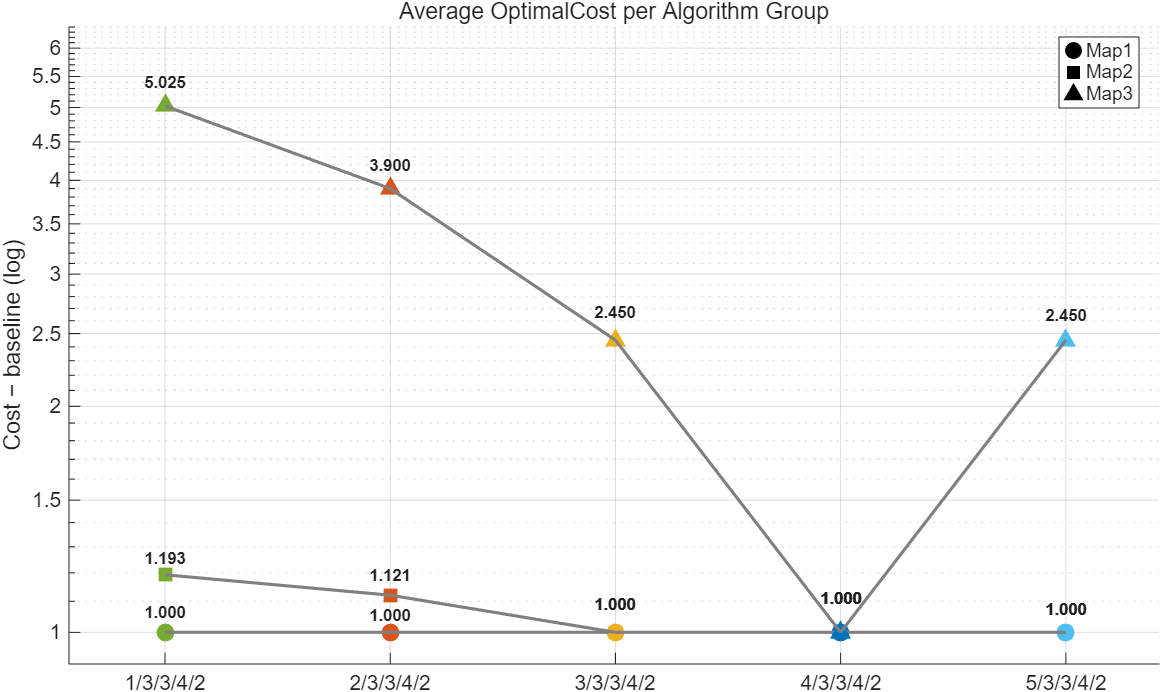
\includegraphics[width=0.32\textwidth]{figures/fig10_cost_nants}\hfil
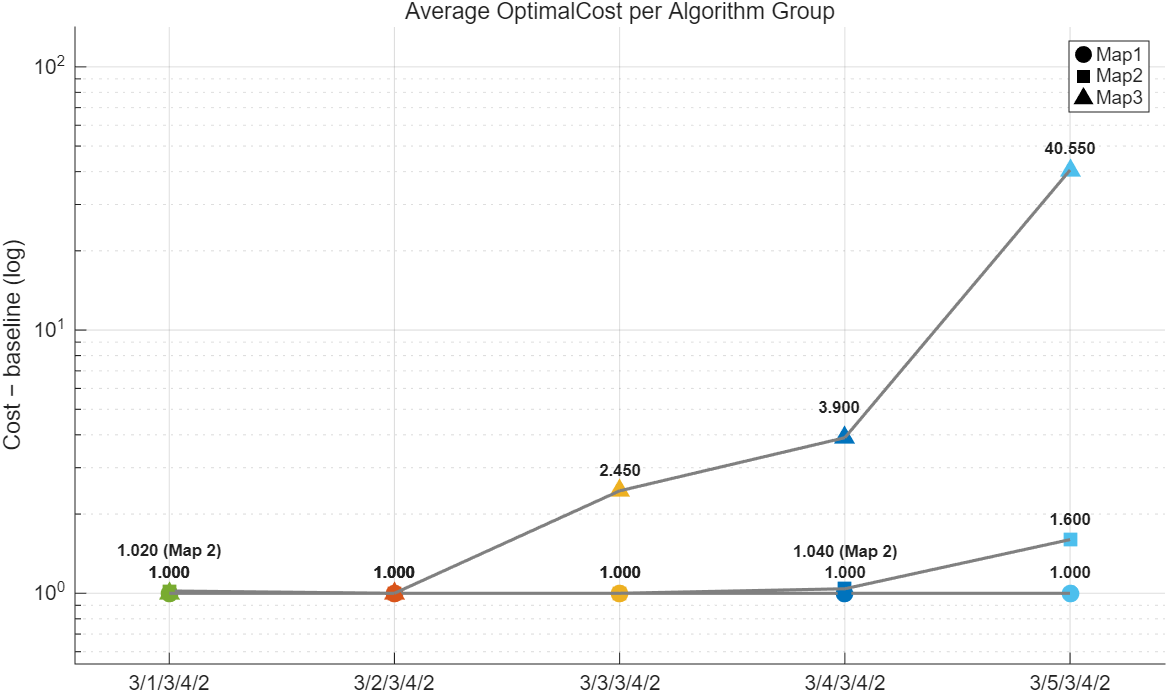
\includegraphics[width=0.32\textwidth]{figures/fig10_cost_q0}\hfil
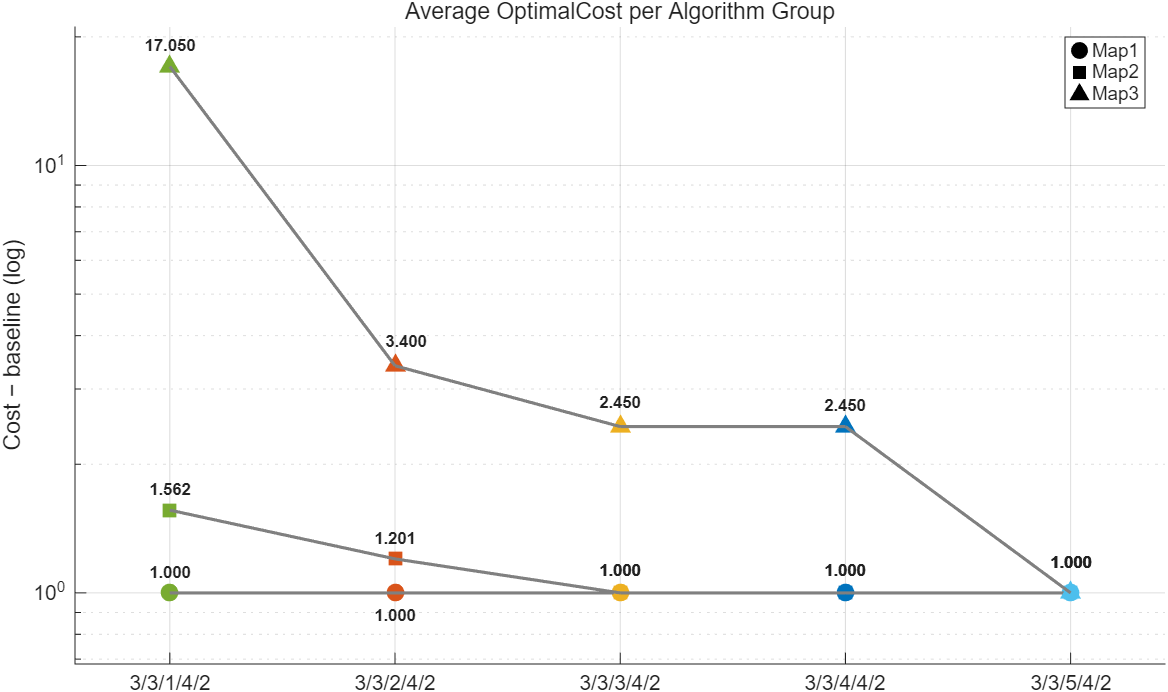
\includegraphics[width=0.32\textwidth]{figures/fig10_cost_ymax}\\
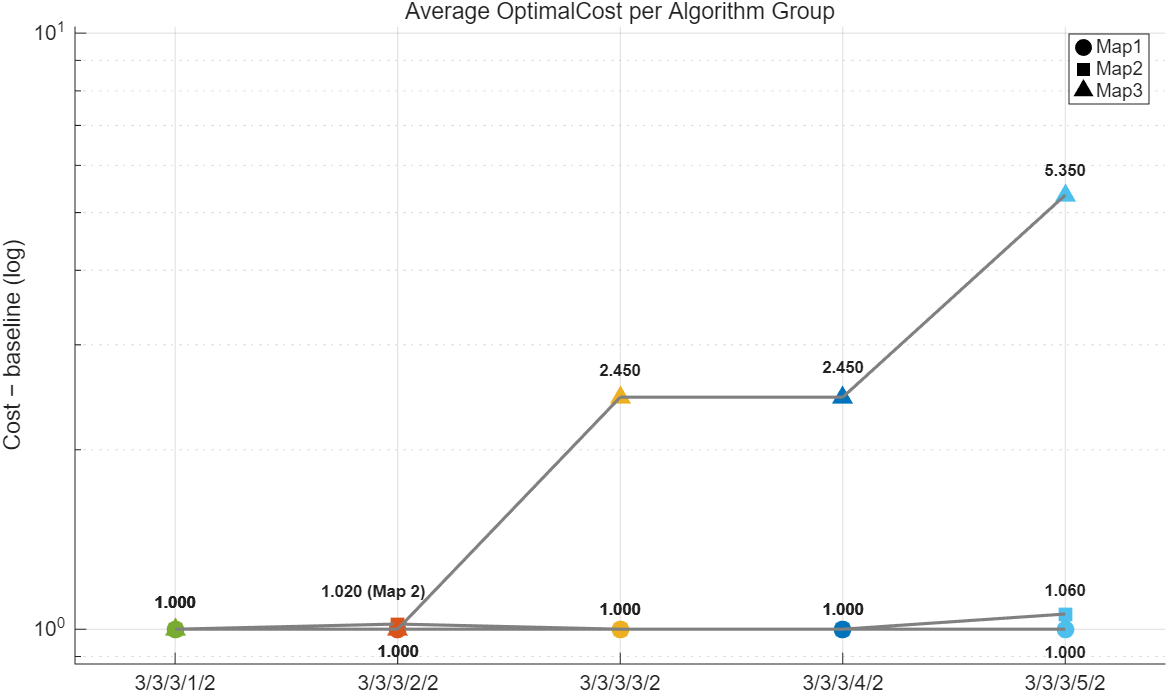
\includegraphics[width=0.32\textwidth]{figures/fig10_cost_relite}\hfil
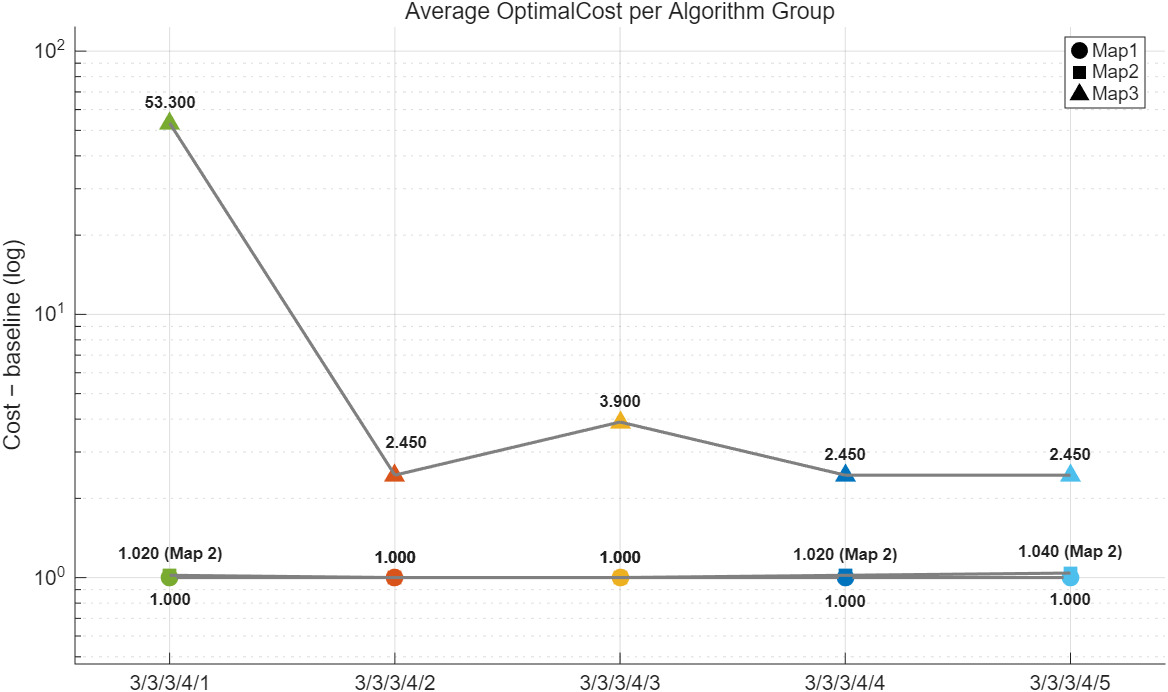
\includegraphics[width=0.32\textwidth]{figures/fig10_cost_k}
\caption{各参数水平在Map~1、Map~2、kroB100上的代价对比。}
\label{fig:sens_cost}
\end{figure*}

\begin{figure*}[!t]

\centering
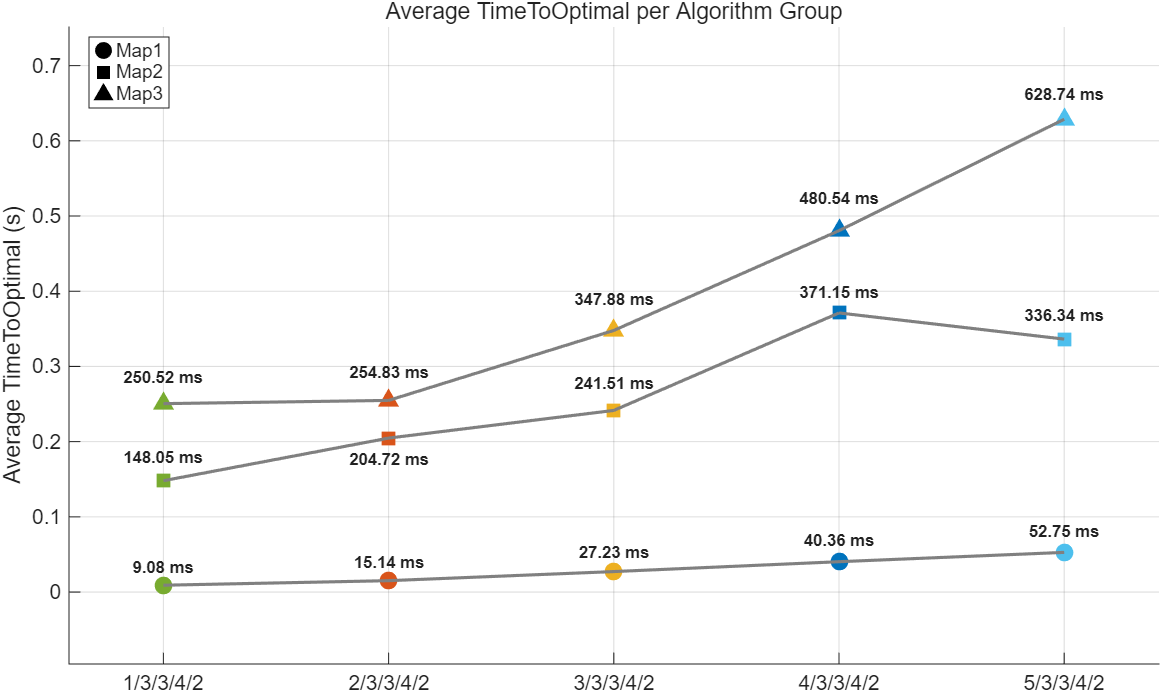
\includegraphics[width=0.32\textwidth]{figures/fig11_time_nants}\hfil
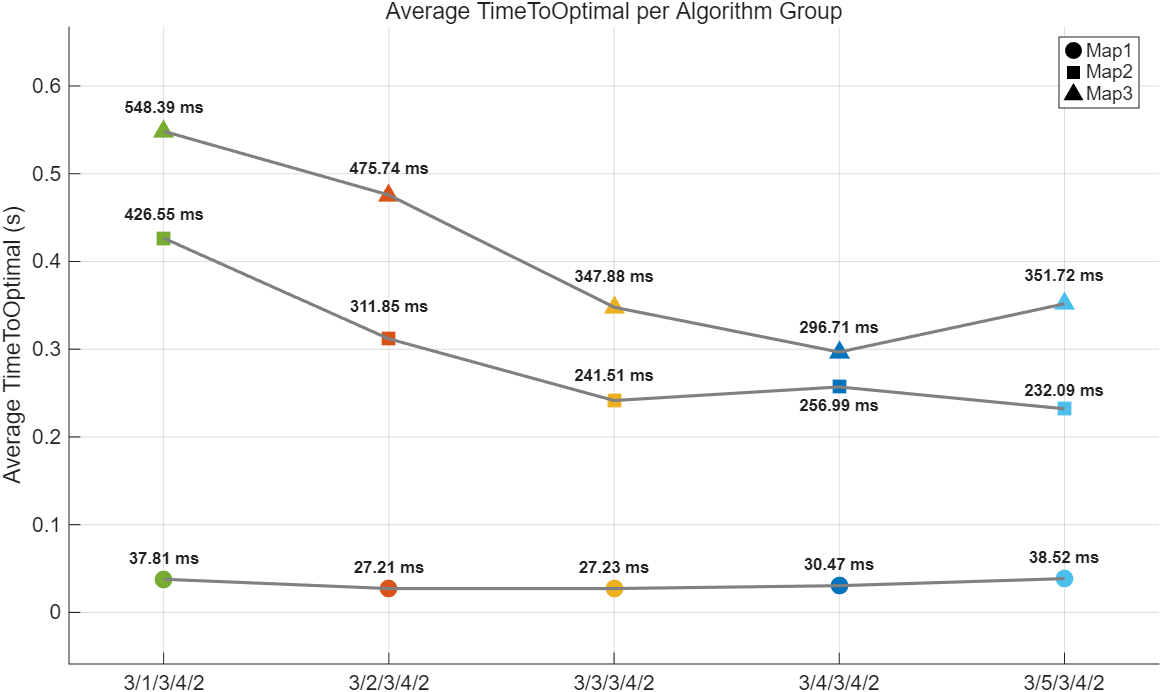
\includegraphics[width=0.32\textwidth]{figures/fig11_time_q0}\hfil
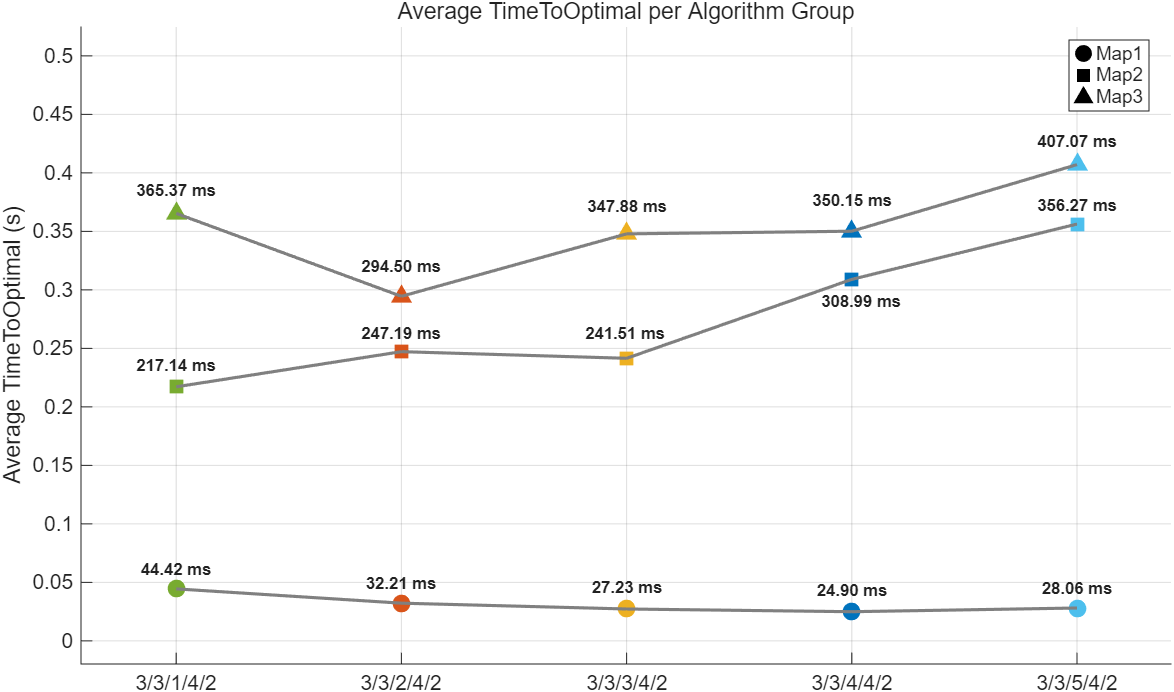
\includegraphics[width=0.32\textwidth]{figures/fig11_time_ymax}\\
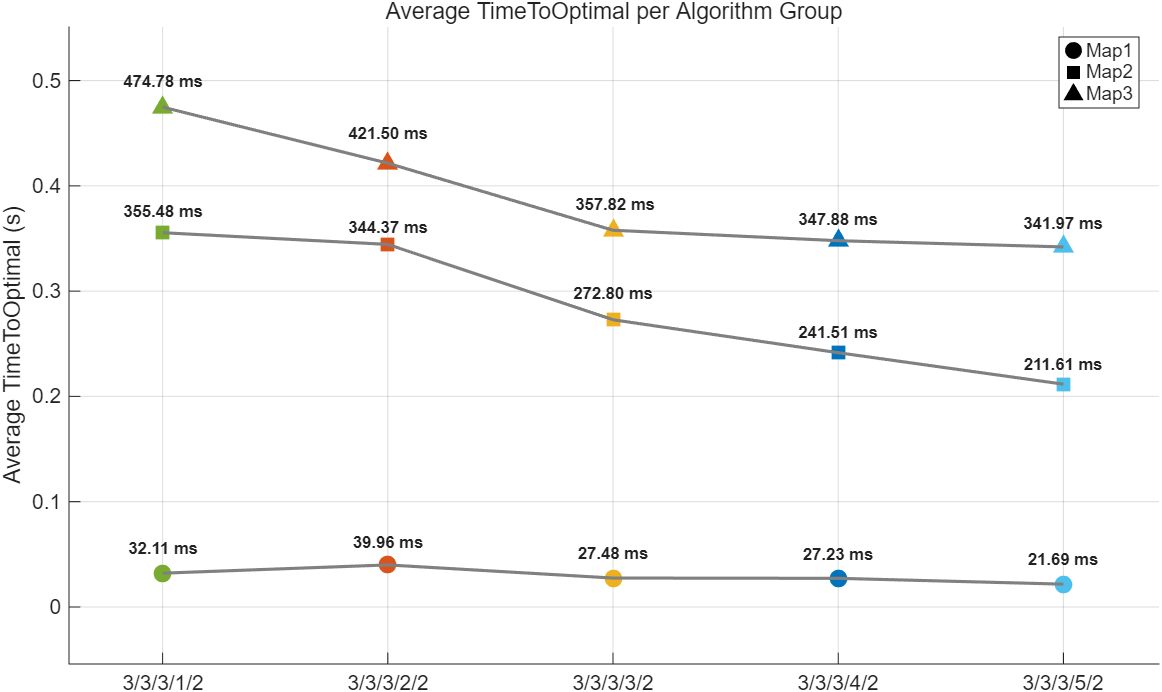
\includegraphics[width=0.32\textwidth]{figures/fig11_time_relite}\hfil
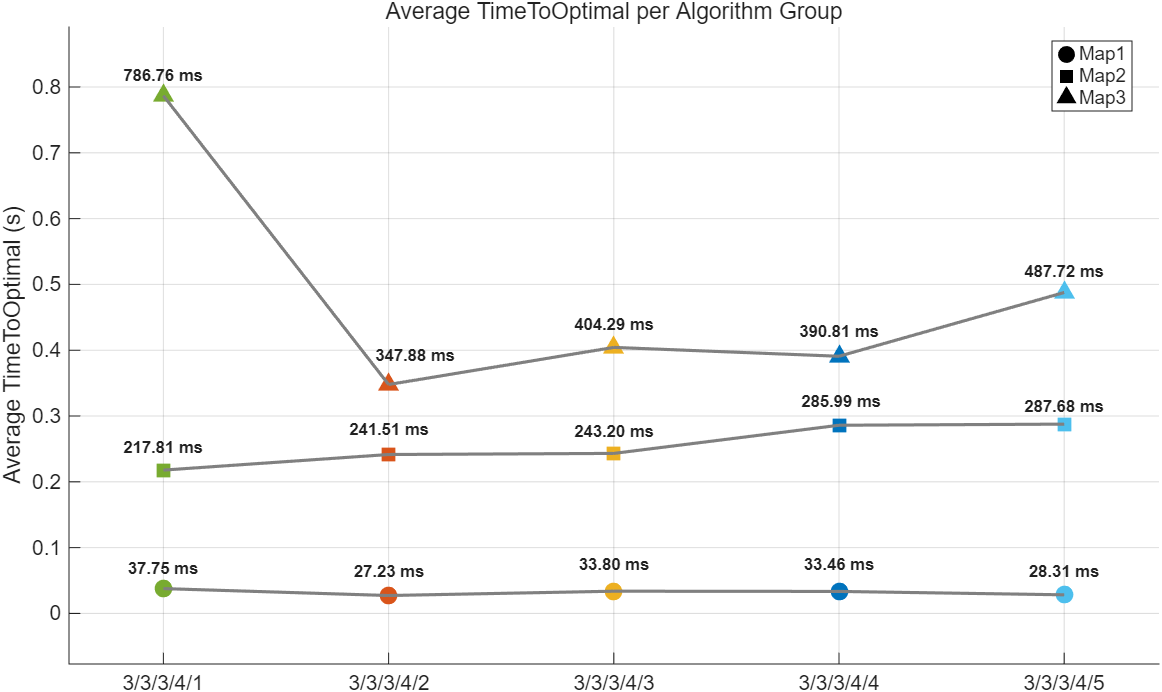
\includegraphics[width=0.32\textwidth]{figures/fig11_time_k}
\caption{各参数水平在Map~1、Map~2、kroB100上的计算时间对比。}
\label{fig:sens_time}
\end{figure*}

\begin{figure}[!t]

\centering
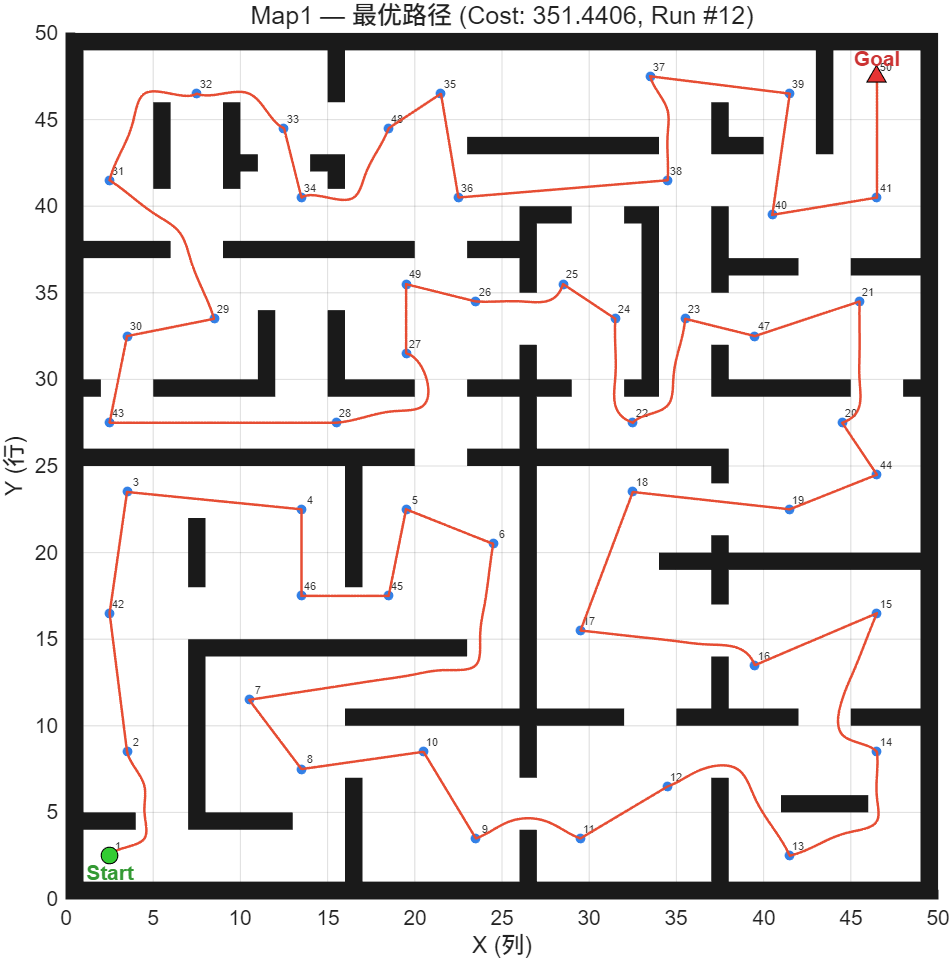
\includegraphics[width=1.05in]{figures/fig12_default_m1}\hfil
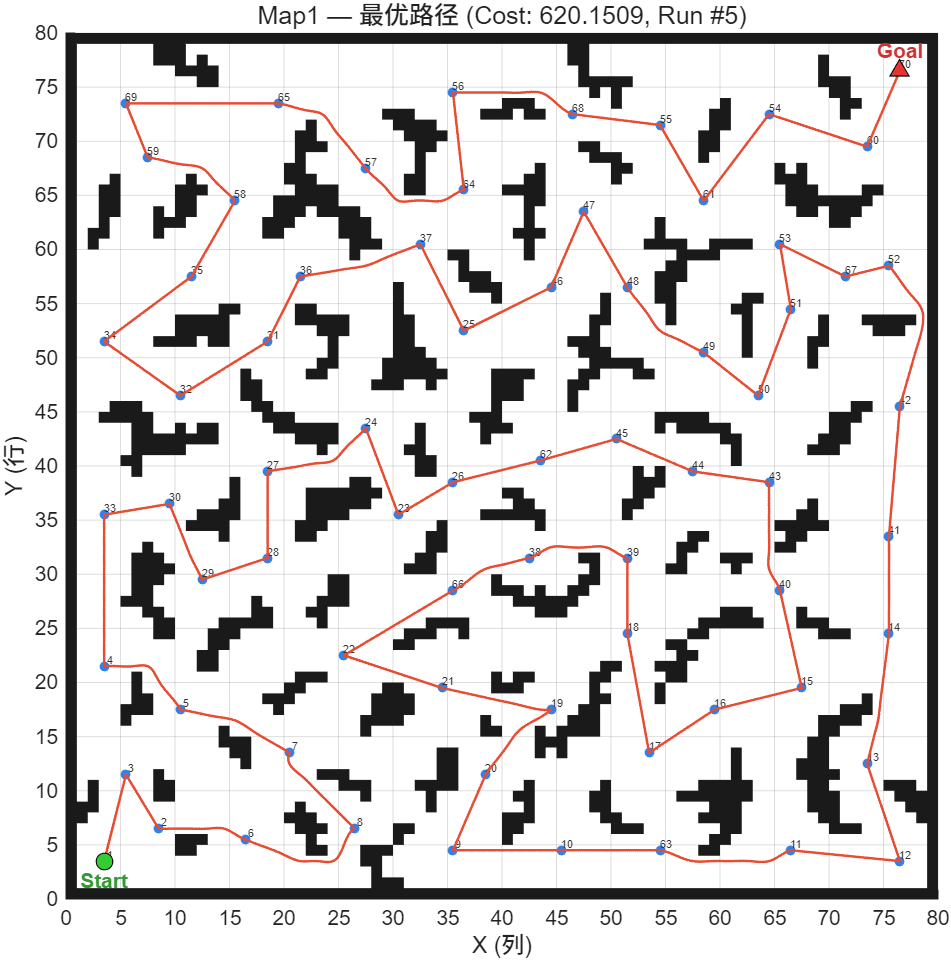
\includegraphics[width=1.05in]{figures/fig12_default_m2}\hfil
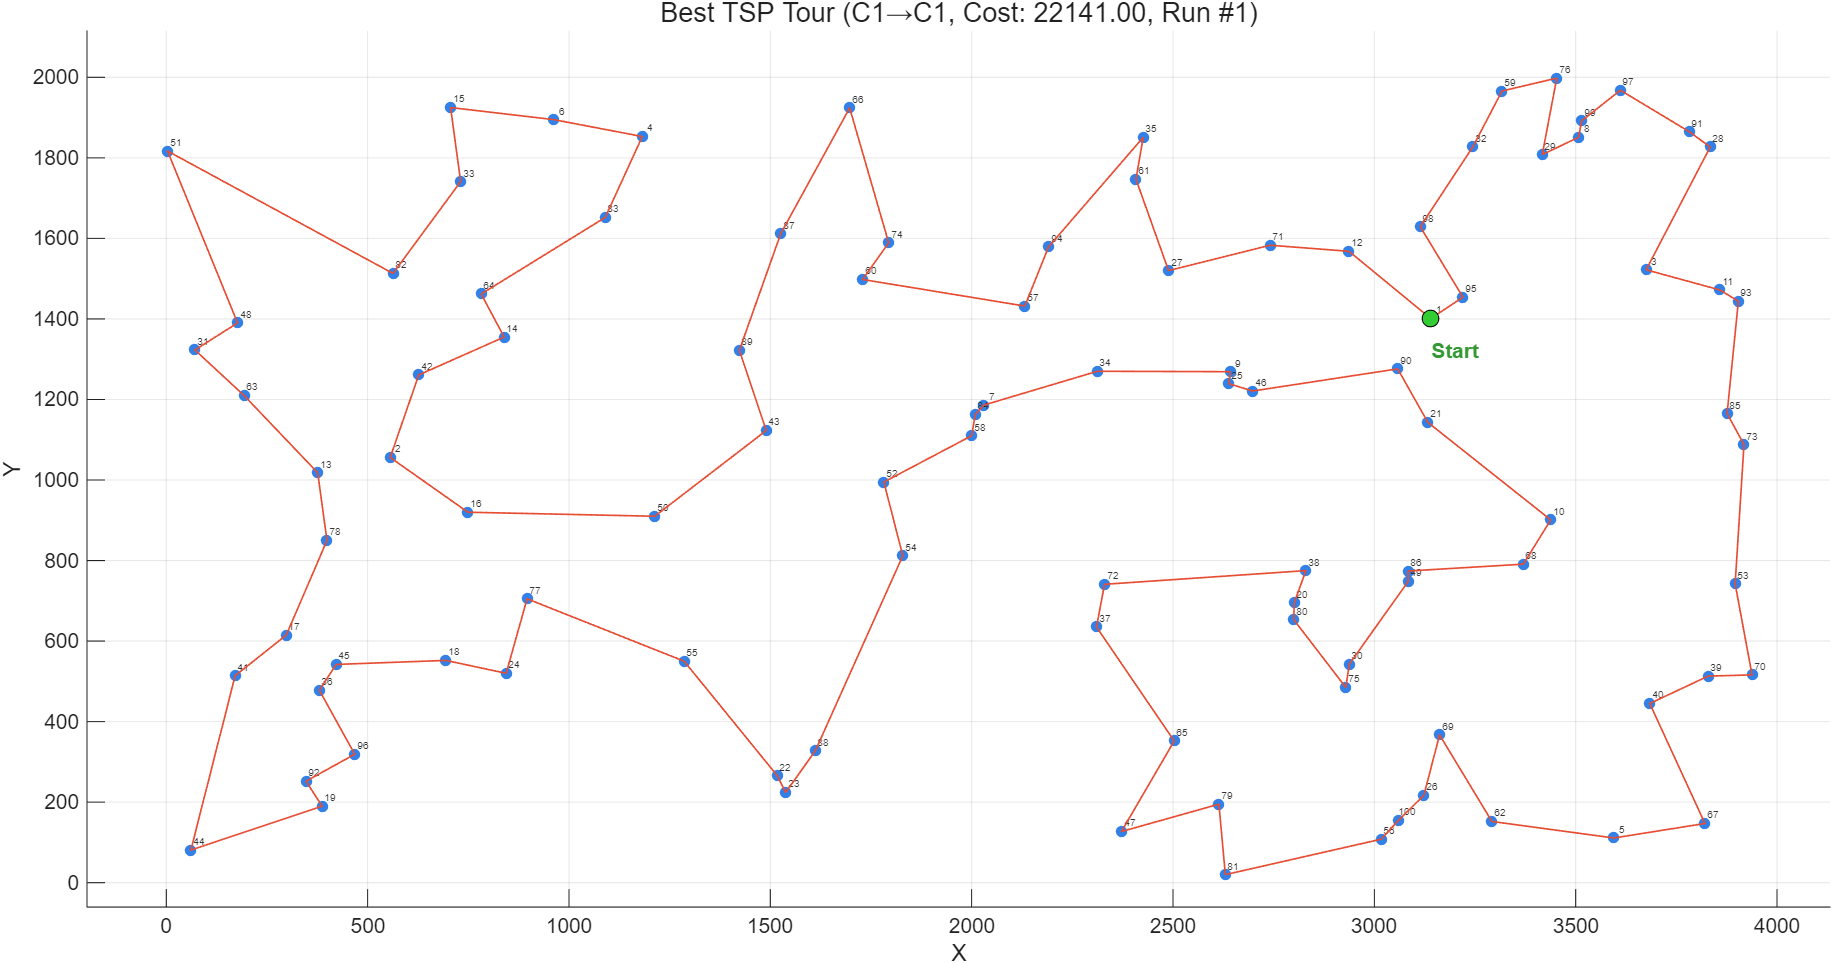
\includegraphics[width=1.05in]{figures/fig12_default_kro}
\caption{默认参数设置下算法在Map~1、Map~2、kroB100上规划的路径图。}
\label{fig:sens_paths}
\end{figure}

\subsection{蚁群优化组件消融实验}

\label{subsec:exp_ablation}

\textbf{目标。} 通过系统性地逐个禁用各组件，隔离改进蚁群优化求解器中每个机制的独立贡献。

\textbf{流程。} 测试六个实验组，每组禁用一个机制，同时保持其他设置不变。表~\ref{tab:ablation_groups}汇总了消融组。

\begin{table}[!t]

\caption{消融实验分组}
\label{tab:ablation_groups}
\centering
\begin{tabular}{cll}
\toprule
组别 & 描述 & 禁用机制 \\
\midrule
1 & 完整算法 & 无 \\
2 & 无伪随机 & ACS伪随机转移规则 \\
3 & 无VND & VND局部搜索 \\
4 & 无S曲线 & 渐进局部搜索调度 \\
5 & 无候选列表 & 候选列表加速 \\
6 & 无MMAS & MMAS信息素边界 \\
\bottomrule
\end{tabular}
\end{table}

\textbf{结果。} 表~\ref{tab:ablation}报告了所有地图上的完整消融结果。消融过程可视化见图~\ref{fig:abl_conv}--\ref{fig:abl_time}。

\begin{table*}[!t]

\caption{消融实验结果}
\label{tab:ablation}
\centering
\scriptsize
\begin{tabular}{llccccccc}
\toprule
组别 & 地图 & 最优代价 & 中位代价 & 平均代价 & 成功率(\%) & 平均时间(s) & 代价极差 & 标准差 \\
\midrule
\multirow{3}{*}{1（完整）}
& Map 1 & 351.4406 & 351.4406 & 351.4406 & 100 & 0.0272 & 0 & 0 \\
& Map 2 & 620.1509 & 620.1509 & 620.1509 & 100 & 0.2415 & 0 & 0 \\
& kroB100 & 22141.0000 & 22141.0000 & 22142.4500 & 97.5 & 0.3479 & 58.00 & 9.1706 \\
\midrule
\multirow{3}{*}{2（无伪随机）}
& Map 1 & 351.4406 & 351.4406 & 351.4406 & 100 & 0.0324 & 0 & 0 \\
& Map 2 & 620.1509 & 620.1509 & 620.1509 & 100 & 0.4157 & 0 & 0 \\
& kroB100 & 22141.0000 & 22141.0000 & 22141.0000 & 100 & 0.7313 & 0 & 0 \\
\midrule
\multirow{3}{*}{3（无VND）}
& Map 1 & 351.4406 & 351.4406 & 352.5747 & 67.5 & 0.1339 & 9.7568 & 2.2744 \\
& Map 2 & 620.9552 & 620.1509 & 632.6061 & 2.5 & 0.5695 & 37.4366 & 8.7702 \\
& kroB100 & 22279.0000 & 22512.0000 & 22566.9750 & 0 & 1.4739 & 1012.0000 & 239.4130 \\
\midrule
\multirow{3}{*}{4（无S曲线）}
& Map 1 & 351.4406 & 351.4406 & 351.4406 & 100 & 0.0175 & 0 & 0 \\
& Map 2 & 620.1509 & 620.1509 & 620.1711 & 97.5 & 0.3494 & 0.8042 & 0.1272 \\
& kroB100 & 22141.0000 & 22141.0000 & 22146.8000 & 90 & 0.6570 & 58.0000 & 17.6217 \\
\midrule
\multirow{3}{*}{5（无候选列表）}
& Map 1 & 351.4406 & 351.4406 & 351.4406 & 100 & 0.0325 & 0 & 0 \\
& Map 2 & 620.1509 & 620.1509 & 620.1509 & 100 & 0.3325 & 0 & 0 \\
& kroB100 & 22141.0000 & 22141.0000 & 22143.9000 & 95 & 0.4260 & 58.0000 & 12.8018 \\
\midrule
\multirow{3}{*}{6（无MMAS）}
& Map 1 & 351.4406 & 353.2976 & 359.6359 & 30 & 0.0218 & 45.0453 & 12.4797 \\
& Map 2 & 620.1509 & 624.1322 & 626.1160 & 10 & 0.0854 & 24.7496 & 6.1209 \\
& kroB100 & 22141.0000 & 22141.0000 & 22166.6500 & 70 & 0.2484 & 235.0000 & 47.4933 \\
\bottomrule
\end{tabular}
\end{table*}

\textbf{分析。} 消融结果揭示了组件重要性的清晰层次。最关键的组件是VND局部搜索（组3）：禁用后kroB100成功率崩溃至0\%，平均代价从22142.45增至22566.98（退化1.9\%），标准差膨胀至239.41。这证实VND对逃脱局部最优和实现近优解不可或缺。第二关键的组件是MMAS信息素边界（组6）：移除后Map~1成功率降至30\%、Map~2降至10\%，代价方差显著，证明信息素边界控制对防止过早收敛至关重要。伪随机转移规则（组2）和S曲线调度（组4）的影响更温和：移除伪随机规则实际上维持了100\%成功率（以稍长运行时间为代价），而移除S曲线使kroB100性能轻微退化（成功率从97.5\%降至90\%）。候选列表加速（组5）对解质量的影响最小——这与其作为纯计算加速器的角色一致——同时提供运行时间收益。总体而言，消融实验证实VND和MMAS是解质量的两大支柱，而伪随机规则、S曲线和候选列表主要贡献于收敛速度和计算效率。消融收敛曲线、代价分布与平均代价/时间对比分别如图~\ref{fig:abl_conv}--\ref{fig:abl_time}所示。

\begin{figure*}[!t]

\centering
\subfloat[Map~1]{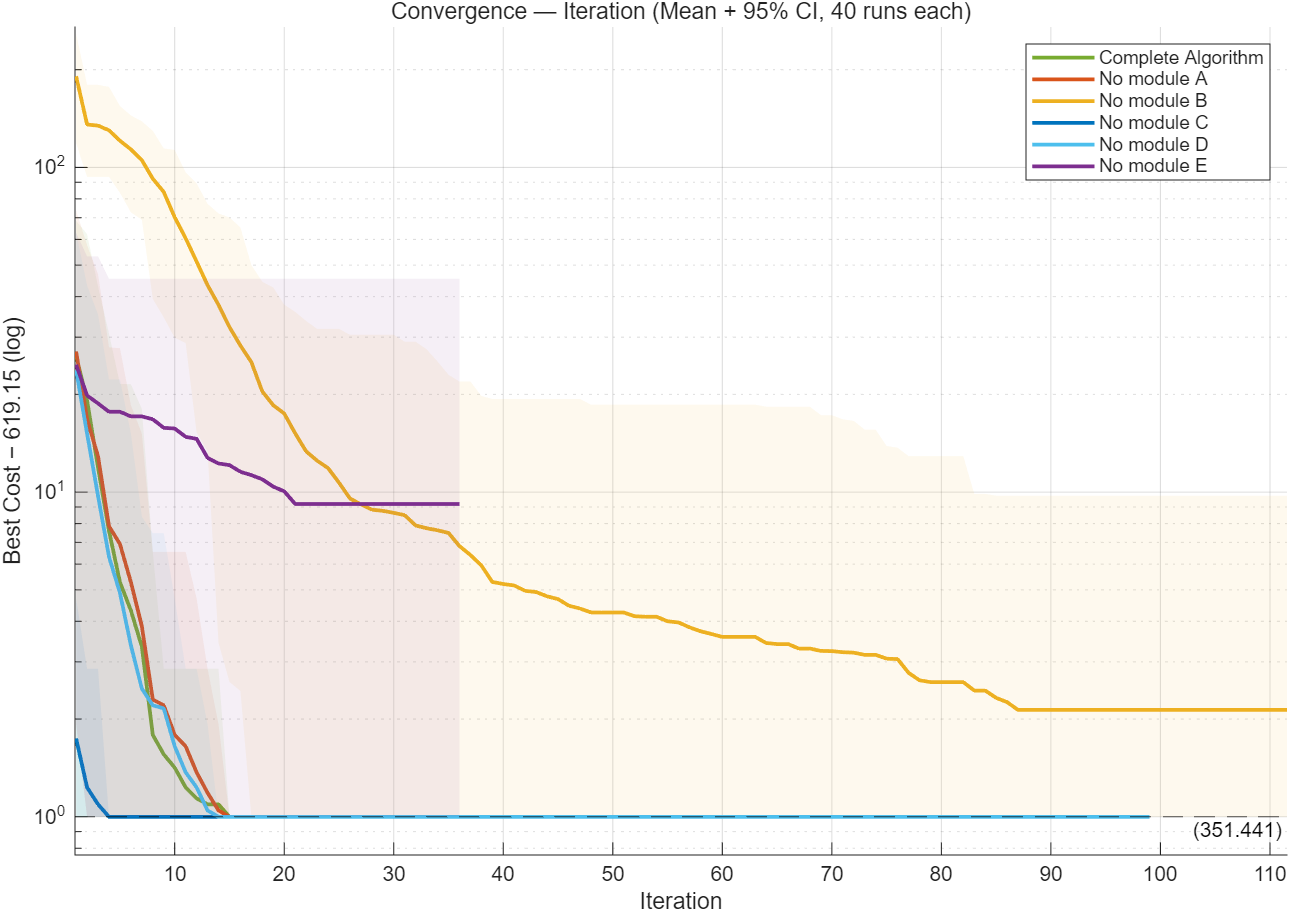
\includegraphics[width=0.3\textwidth]{figures/fig13a_conv_m1}\label{fig:abl_conv_a}}\hfil
\subfloat[Map~2]{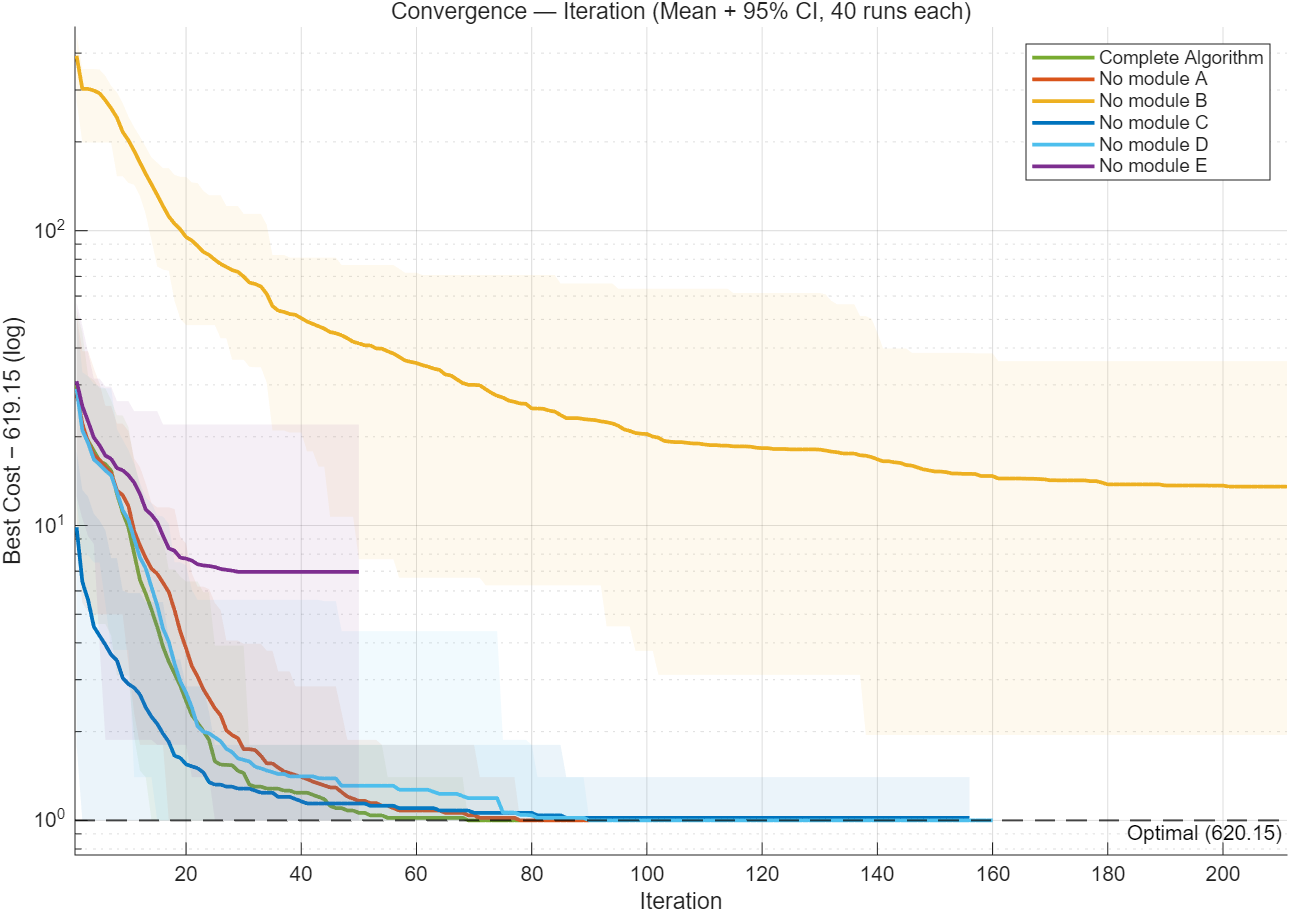
\includegraphics[width=0.3\textwidth]{figures/fig13b_conv_m2}\label{fig:abl_conv_b}}\hfil
\subfloat[kroB100]{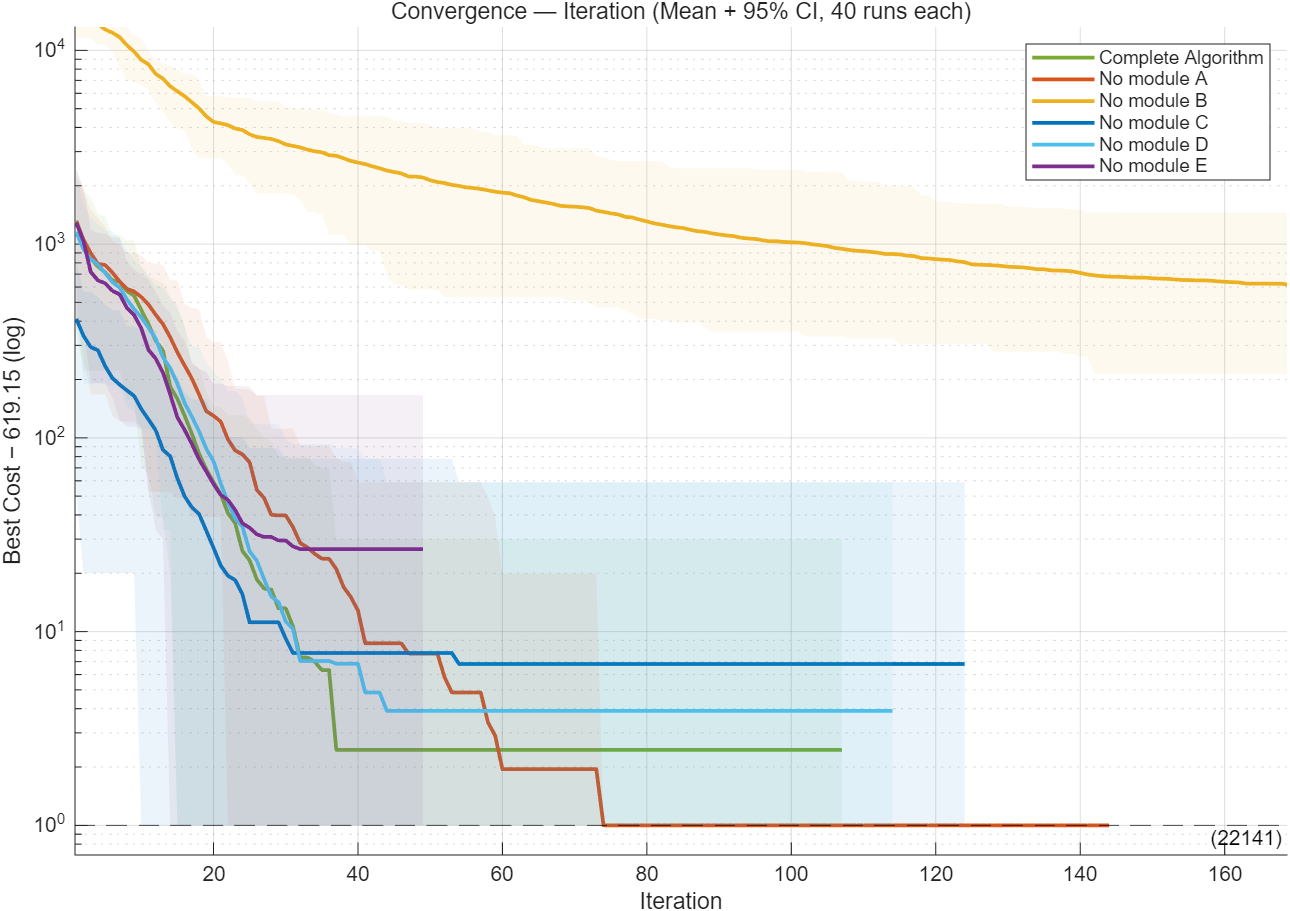
\includegraphics[width=0.3\textwidth]{figures/fig13c_conv_kro}\label{fig:abl_conv_c}}
\caption{六个消融组在三张地图上40次运行的平均迭代次数-代价收敛曲线。}
\label{fig:abl_conv}
\end{figure*}

\begin{figure*}[!t]

\centering
\subfloat[Map~1]{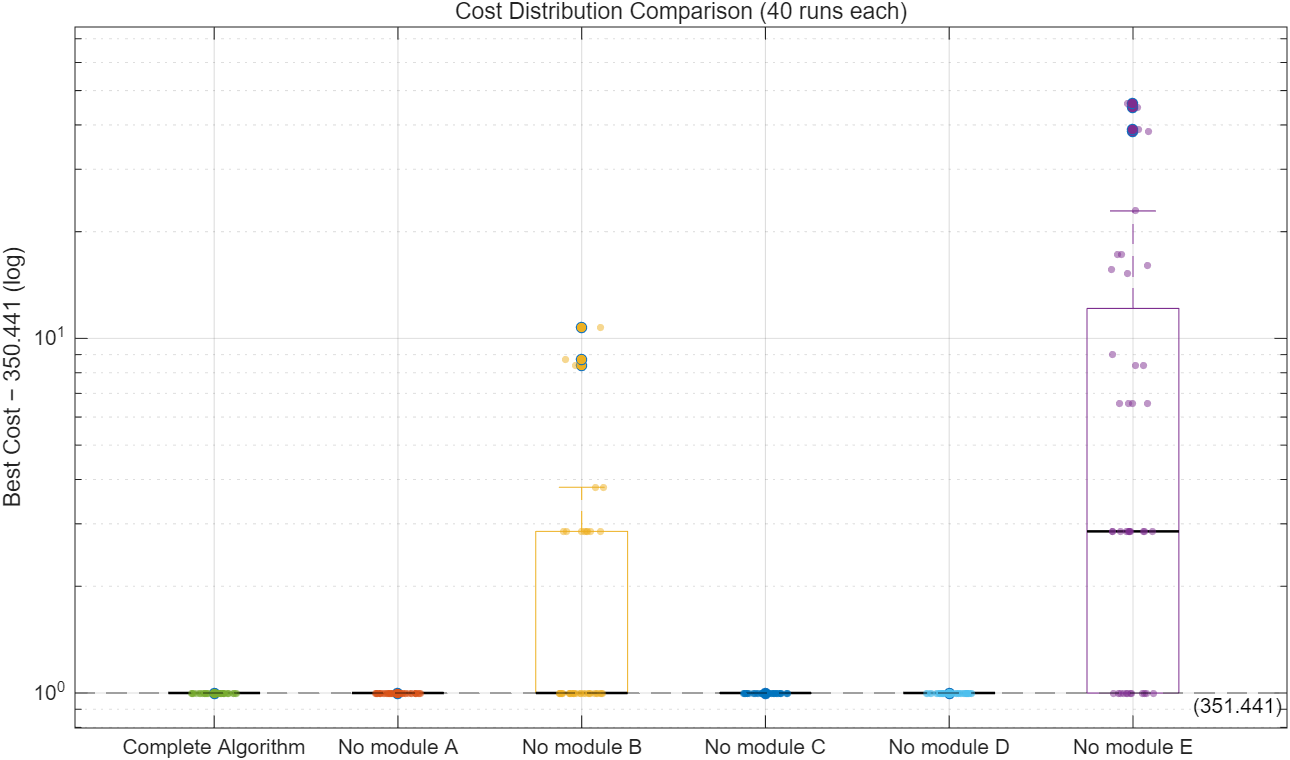
\includegraphics[width=0.3\textwidth]{figures/fig14a_box_m1}}\hfil
\subfloat[Map~2]{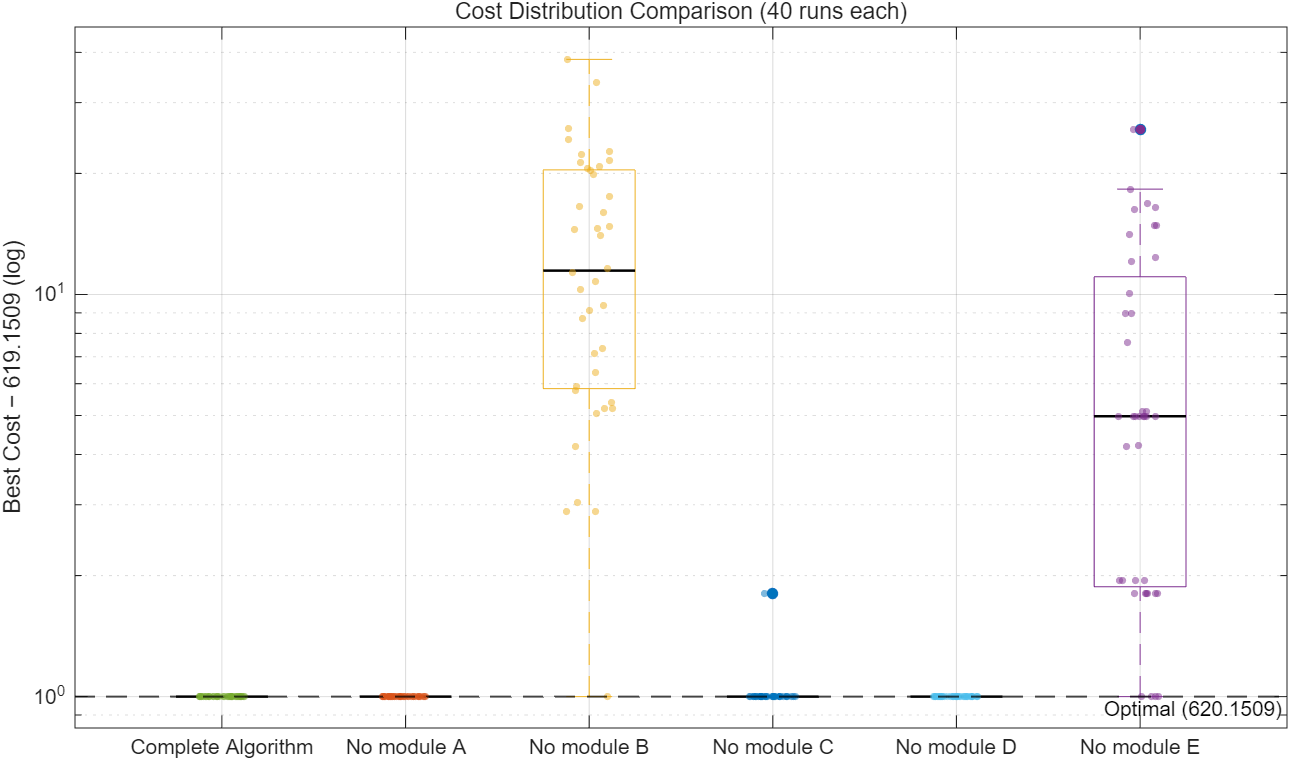
\includegraphics[width=0.3\textwidth]{figures/fig14b_box_m2}}\hfil
\subfloat[kroB100]{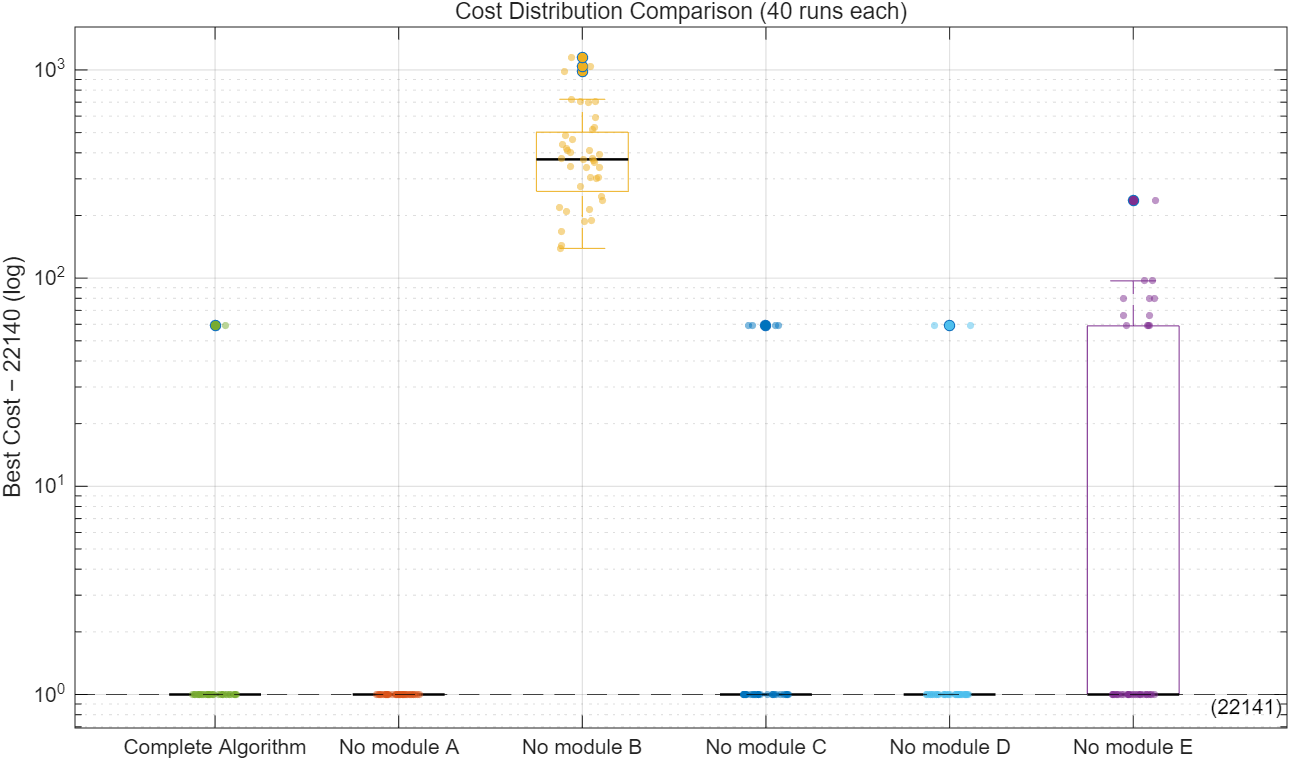
\includegraphics[width=0.3\textwidth]{figures/fig14c_box_kro}}
\caption{六个消融组在三张地图上40次运行的代价分布（箱线图）。}
\label{fig:abl_box}
\end{figure*}

\begin{figure*}[!t]

\centering
\subfloat[Map~1]{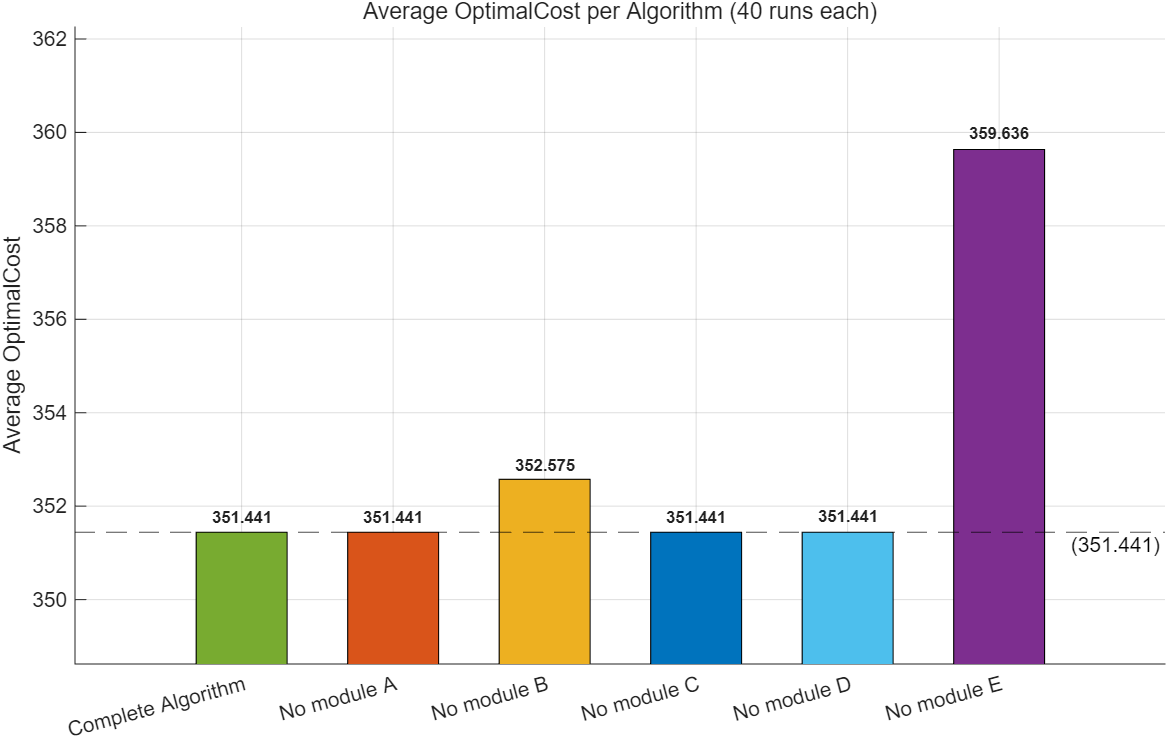
\includegraphics[width=0.3\textwidth]{figures/fig15a_costbar_m1}}\hfil
\subfloat[Map~2]{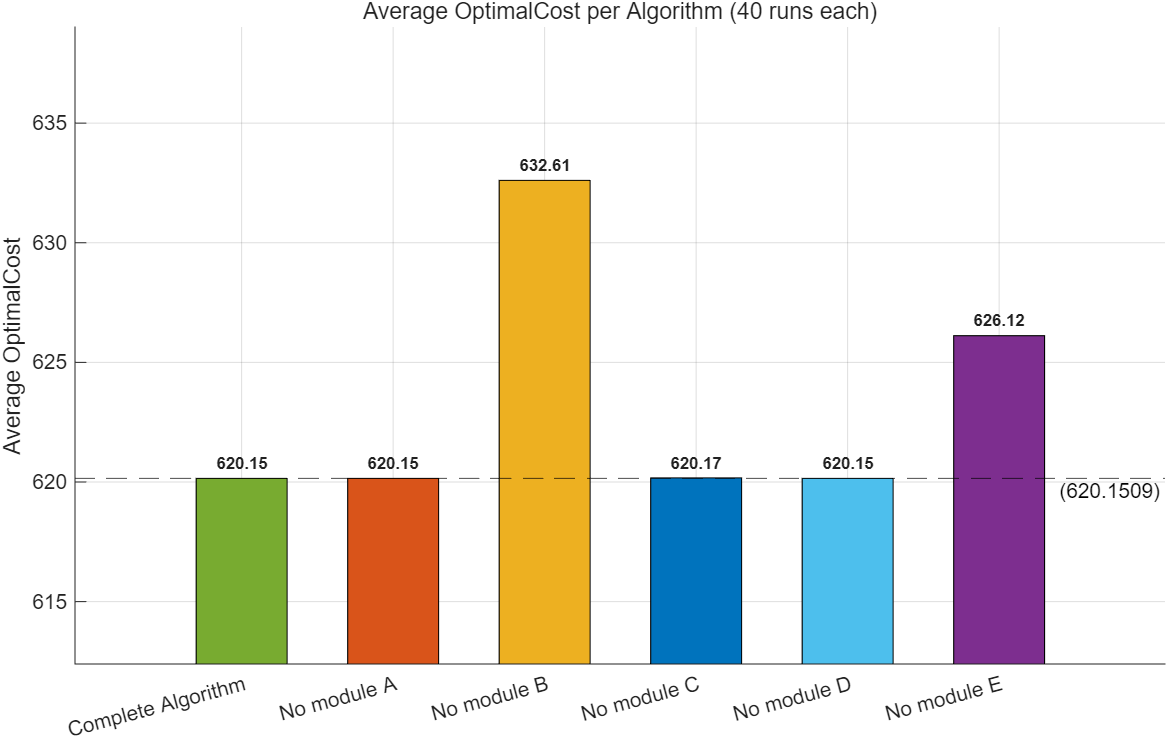
\includegraphics[width=0.3\textwidth]{figures/fig15b_costbar_m2}}\hfil
\subfloat[kroB100]{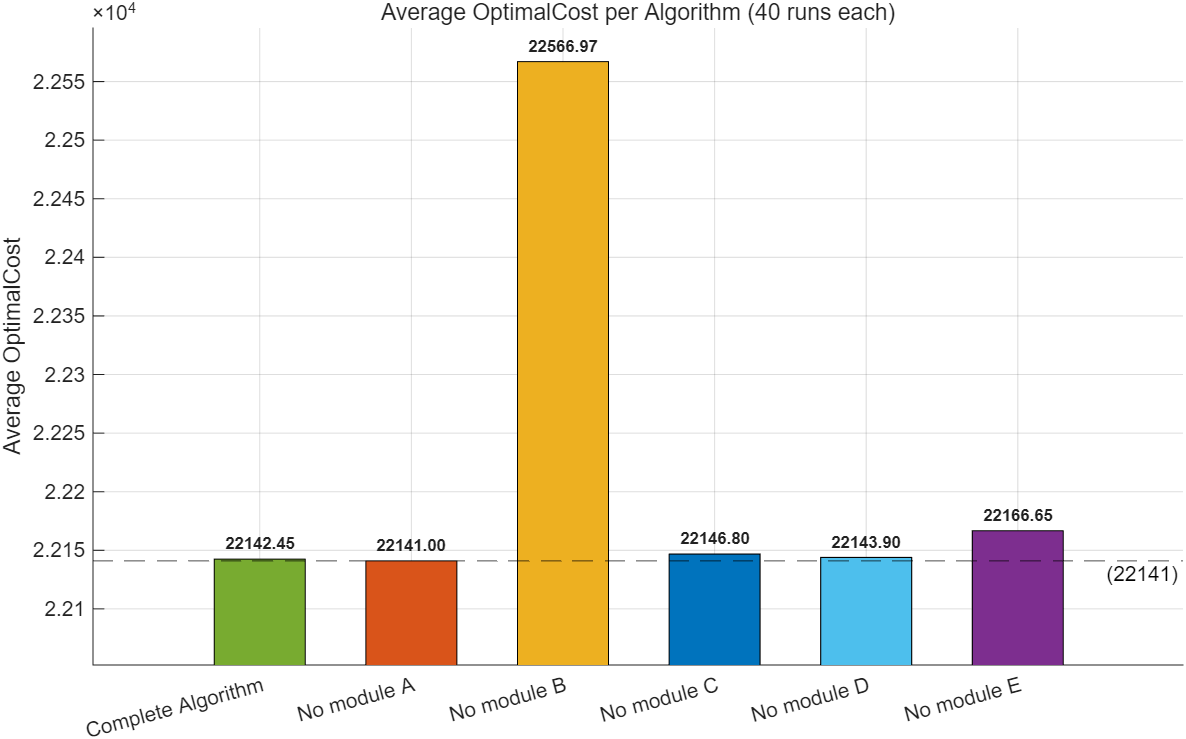
\includegraphics[width=0.3\textwidth]{figures/fig15c_costbar_kro}}
\caption{六个消融组在三张地图上的平均代价对比（柱状图）。}
\label{fig:abl_cost}
\end{figure*}

\begin{figure*}[!t]

\centering
\subfloat[Map~1]{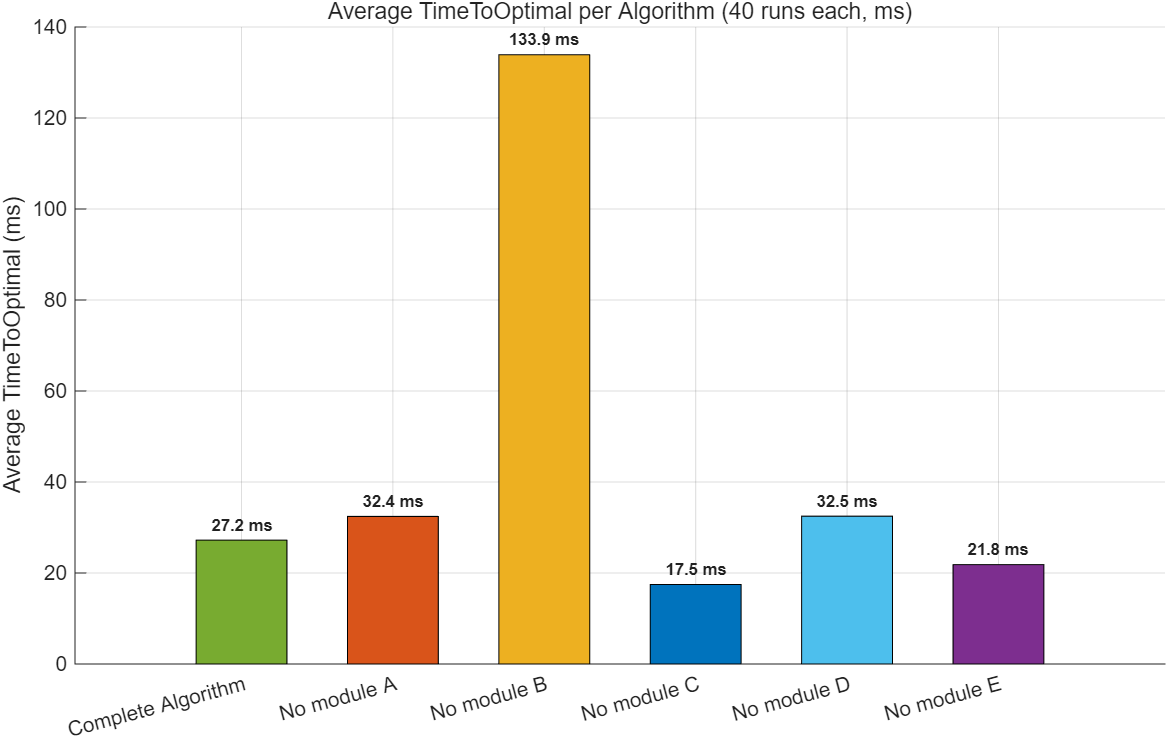
\includegraphics[width=0.3\textwidth]{figures/fig16a_timebar_m1}}\hfil
\subfloat[Map~2]{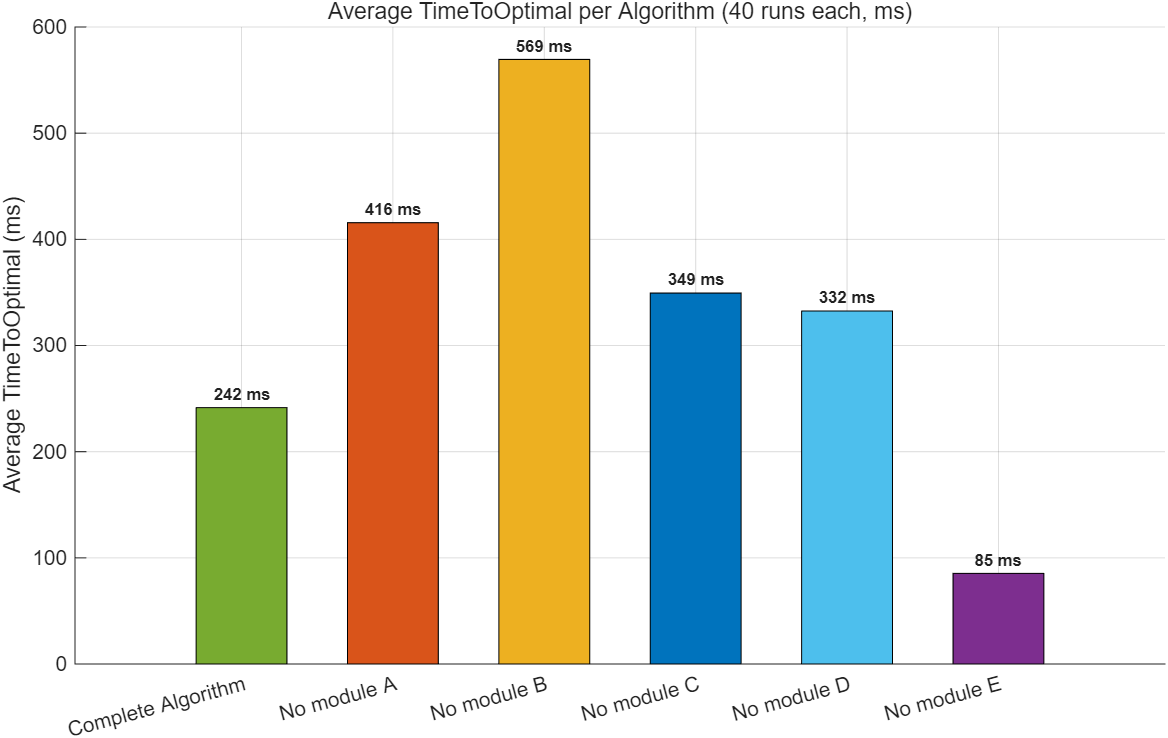
\includegraphics[width=0.3\textwidth]{figures/fig16b_timebar_m2}}\hfil
\subfloat[kroB100]{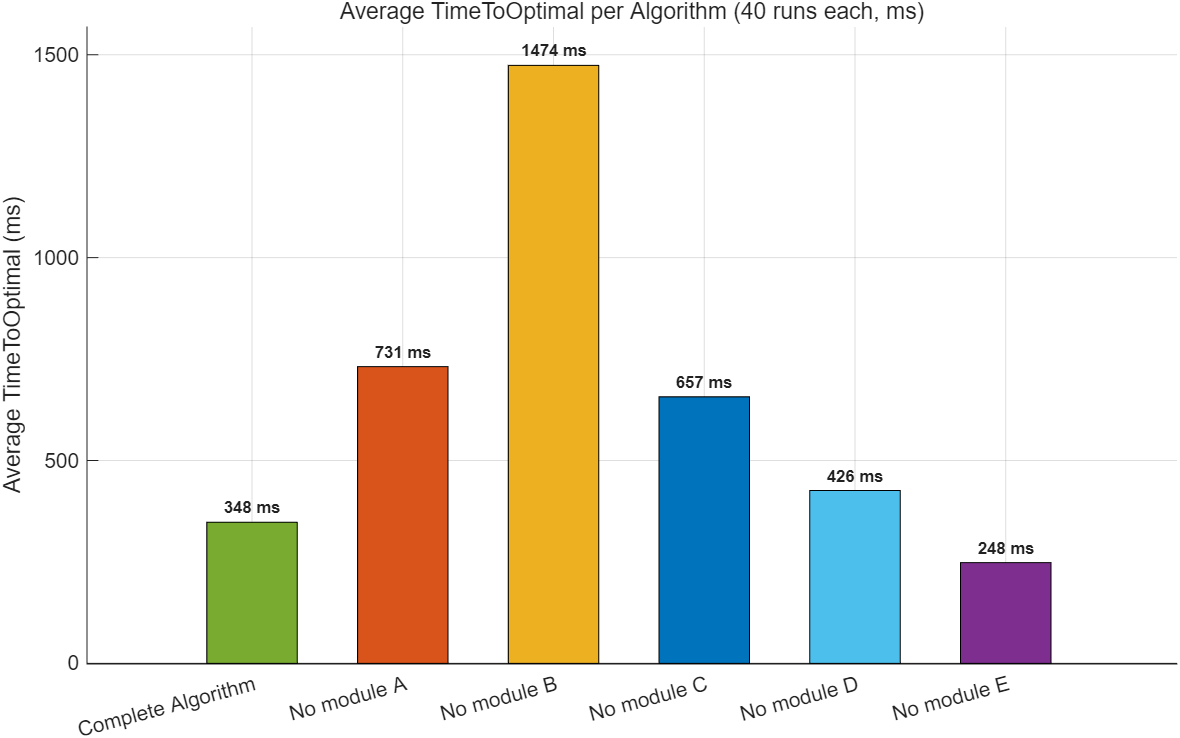
\includegraphics[width=0.3\textwidth]{figures/fig16c_timebar_kro}}
\caption{六个消融组在三张地图上的平均计算时间对比（柱状图）。}
\label{fig:abl_time}
\end{figure*}

\subsection{不同旅行商求解器的多目标点遍历对比}

\label{subsec:exp_cmp}

\textbf{目标。} 通过将改进A*规划器（结合虚拟节点法）与不同旅行商求解器结合，评估完整的多目标点遍历框架，并将所提蚁群优化求解器（MMAS-VND-CL）与基线旅行商元启发式方法进行对比。

\textbf{流程。} 四个旅行商求解器——所提MMAS-VND-CL（TSP\_ACO\_v2\_4）、标准蚁群系统（ACO）、遗传算法（GA）和模拟退火（SA）——分别与改进A*规划器结合，在所有三张地图上求解多目标点遍历问题。每个求解器的参数汇总于表~\ref{tab:tsp_params}。每种组合在每张地图上运行40次。MMAS-VND-CL的完整参数为：蚂蚁数$m=40$，$\alpha=1$，$\beta=2$，$\rho=0.25$，$Q=225$，$\tau_0=0.1$，最大迭代200，$q_0=0.45$，$y_{\max}=0.4$，转换区间$[0,30]$，精英比率$r_{\mathrm{elite}}=0.7$，候选列表大小$k=9$。

\begin{table}[!t]

\caption{对比旅行商求解器的参数设置}
\label{tab:tsp_params}
\centering
\scriptsize
\begin{tabular}{p{0.22\columnwidth}p{0.68\columnwidth}}
\toprule
算法 & 参数 \\
\midrule
MMAS-VND-CL & 蚂蚁数量$m=40$；信息素启发因子$\alpha=1$；期望启发因子$\beta=2$；信息素挥发系数$\rho=0.25$；信息素强度$Q=225$；初始信息素$\tau_0=0.1$；迭代次数$\mathrm{Iter}=200$；贪心选择概率$=0.45$；局部搜索比例$=0.4$；局部搜索过渡区间$=[0,30]$；局部搜索精英蚂蚁占比$=0.7$；候选邻居数$=9$ \\
ACO & 蚂蚁数量$m=40$；信息素启发因子$\alpha=1$；期望启发因子$\beta=2$；信息素挥发系数$\rho=0.25$；信息素强度$Q=225$；初始信息素$\tau_0=0.1$；迭代次数$\mathrm{Iter}=100$ \\
GA & 种群规模$\mathrm{Pop}=100$；迭代次数$\mathrm{Iter}=1500$；交叉概率$P_c=0.8$；变异概率$P_m=0.25$；精英保留数量$=10$ \\
SA & 初始温度$T_0=150$；降温系数$\alpha=0.996$；每个温度下的迭代次数$L=10$；终止温度$T_{\mathrm{end}}=10^{-8}$ \\
\bottomrule
\end{tabular}
\end{table}

\textbf{结果。} 表~\ref{tab:tsp_cmp}报告了每个求解器的多目标点遍历性能。对应可视化结果见图~\ref{fig:tsp_conv}--\ref{fig:tsp_paths}。

\begin{table*}[!t]

\caption{多目标点遍历对比结果}
\label{tab:tsp_cmp}
\centering
\begin{tabular}{llccccccc}
\toprule
算法 & 地图 & 最优代价 & 中位代价 & 平均代价 & 命中最优率(\%) & 平均时间(s) & 代价极差 & 标准差 \\
\midrule
\multirow{3}{*}{MMAS-VND-CL（本文）}
& Map 1 & 351.4406 & 351.4406 & 351.4406 & 100 & 0.0272 & 0 & 0 \\
& Map 2 & 620.1509 & 620.1509 & 620.1509 & 100 & 0.2415 & 0 & 0 \\
& kroB100 & 22141.0000 & 22141.0000 & 22142.4500 & 97.5 & 0.3479 & 58.00 & 9.1706 \\
\midrule
\multirow{3}{*}{ACO}
& Map 1 & 359.3170 & 388.5591 & 388.6513 & 0 & 0.0564 & 59.3454 & 15.5736 \\
& Map 2 & 638.6843 & 688.3238 & 685.7453 & 0 & 0.1304 & 88.0149 & 18.9081 \\
& kroB100 & 23359.0000 & 24418.5000 & 24435.8250 & 0 & 0.3300 & 2045.0000 & 559.3037 \\
\midrule
\multirow{3}{*}{GA}
& Map 1 & 404.4468 & 482.2940 & 485.1563 & 0 & 3.0007 & 201.4194 & 44.2581 \\
& Map 2 & 698.4059 & 859.9173 & 851.2521 & 0 & 3.8424 & 221.8002 & 46.5627 \\
& kroB100 & 33271.0000 & 37285.5000 & 37360.6500 & 0 & 4.9882 & 14912.0000 & 2680.1153 \\
\midrule
\multirow{3}{*}{SA}
& Map 1 & 359.9775 & 394.8159 & 390.3485 & 0 & 0.3902 & 44.3223 & 13.9440 \\
& Map 2 & 664.5622 & 688.7545 & 691.9980 & 0 & 0.7321 & 17.4566 & 66.3322 \\
& kroB100 & 23574.0000 & 24817.5000 & 24918.3500 & 0 & 0.3218 & 2841.0000 & 752.5199 \\
\bottomrule
\end{tabular}
\end{table*}

\textbf{分析。} 所提MMAS-VND-CL求解器在所有地图上均显著优于三个基线。在kroB100（最优代价22141）上，所提求解器以97.5\%的命中率达到最优代价，平均代价为22142.45，而最优基线（ACO）的平均代价为24435.83——退化10.4\%——且从未命中最优代价。GA表现最差，kroB100上平均代价37360.65，高于最优68.7\%。性能差距在稳定性方面更为显著：所提求解器的标准差（9.17）比GA（2680.12）小60倍以上，比SA（752.52）小82倍以上，展现出卓越的可靠性。Map~1和Map~2上100\%的命中最优率表明所提求解器在这两个环境中稳定找到全局最优，而所有基线均从未命中最优。在计算时间方面，所提求解器与ACO相当（kroB100上0.35~s对比0.33~s），显著快于GA（4.99~s），尽管包含了VND局部搜索——此收益归功于候选列表加速。这些结果证实，将基于JPS的A*规划器与虚拟节点MMAS-VND-CL蚁群优化求解器集成的框架，在障碍环境多目标点遍历路径规划中提供了卓越的解质量、可靠性和效率。收敛曲线、代价分布、平均代价/时间以及最优路径分别如图~\ref{fig:tsp_conv}--\ref{fig:tsp_paths}所示。

\begin{figure*}[!t]

\centering
\subfloat[Map~1]{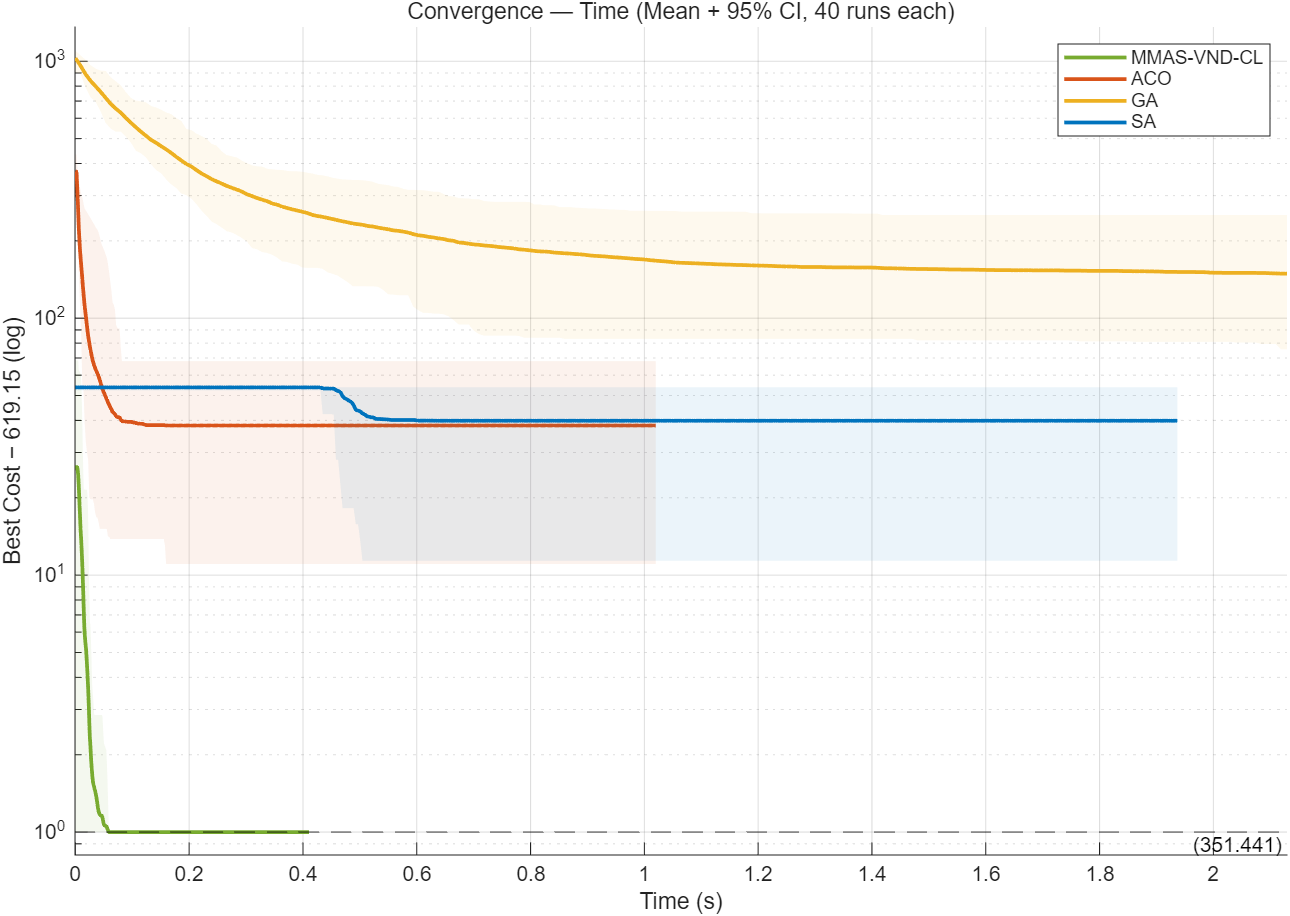
\includegraphics[width=0.3\textwidth]{figures/fig17a_tspconv_m1}}\hfil
\subfloat[Map~2]{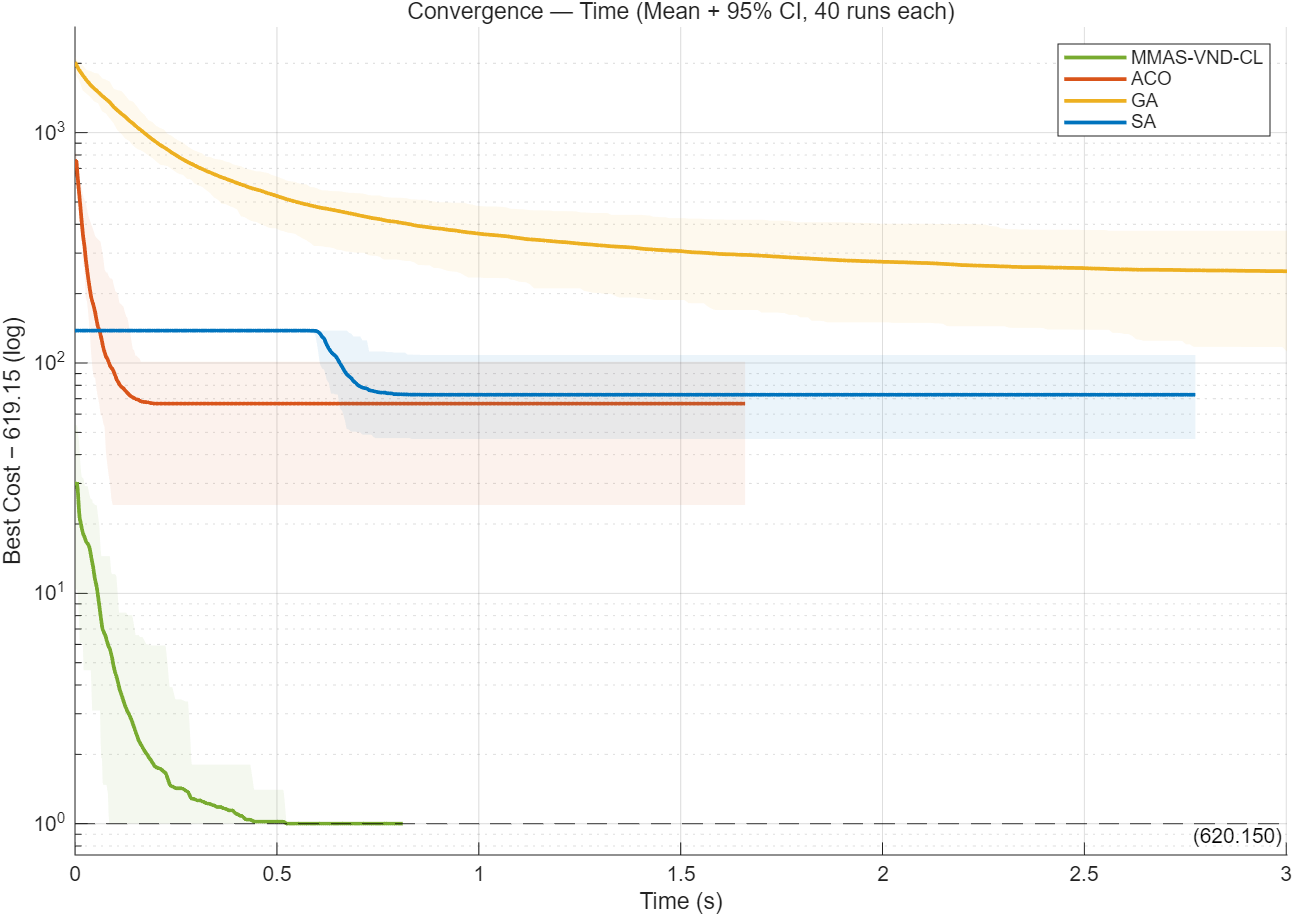
\includegraphics[width=0.3\textwidth]{figures/fig17b_tspconv_m2}}\hfil
\subfloat[kroB100]{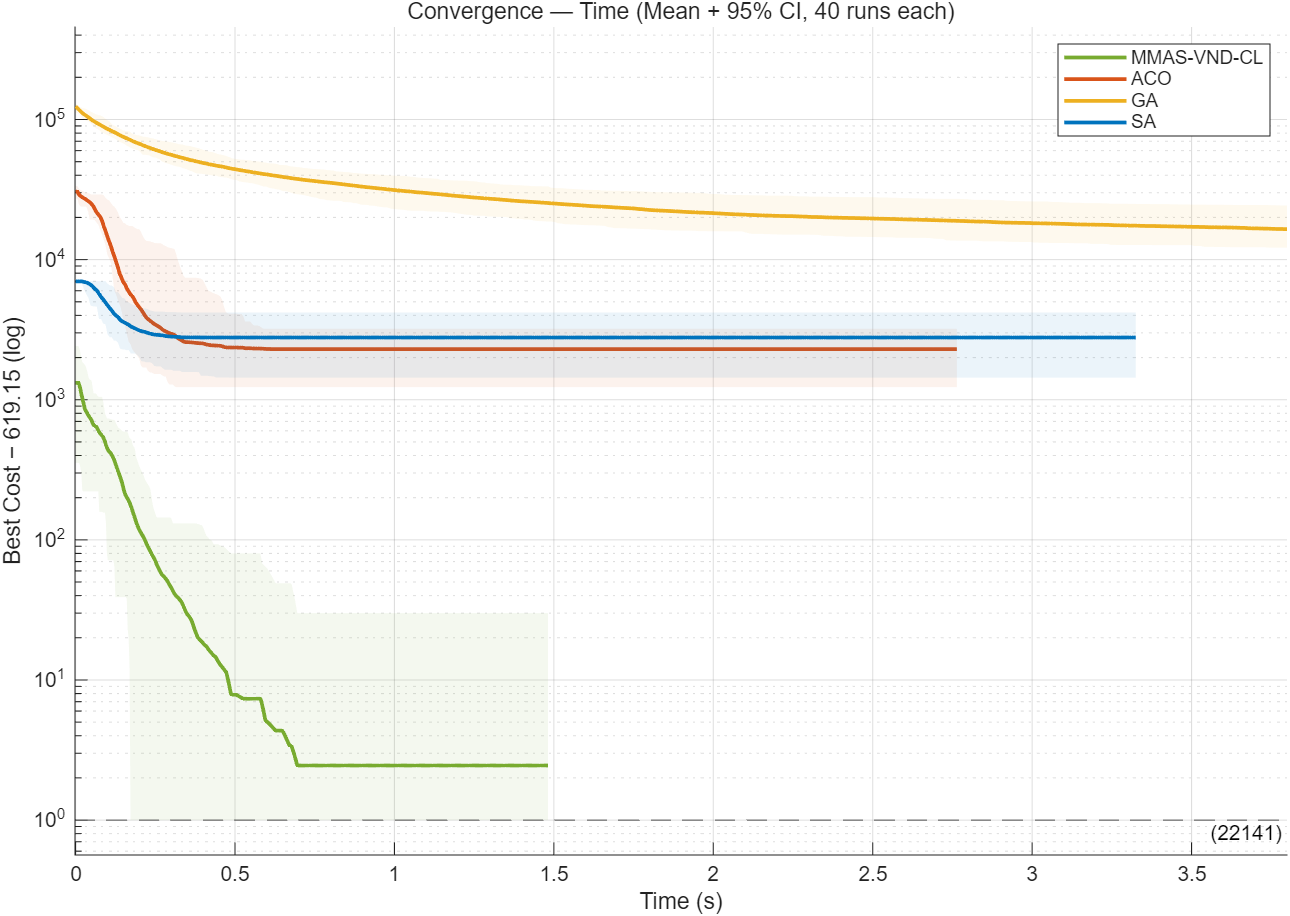
\includegraphics[width=0.3\textwidth]{figures/fig17c_tspconv_m3}}
\caption{四个旅行商求解器在三张地图上40次运行的平均时间-代价收敛曲线。}
\label{fig:tsp_conv}
\end{figure*}

\begin{figure*}[!t]

\centering
\subfloat[Map~1]{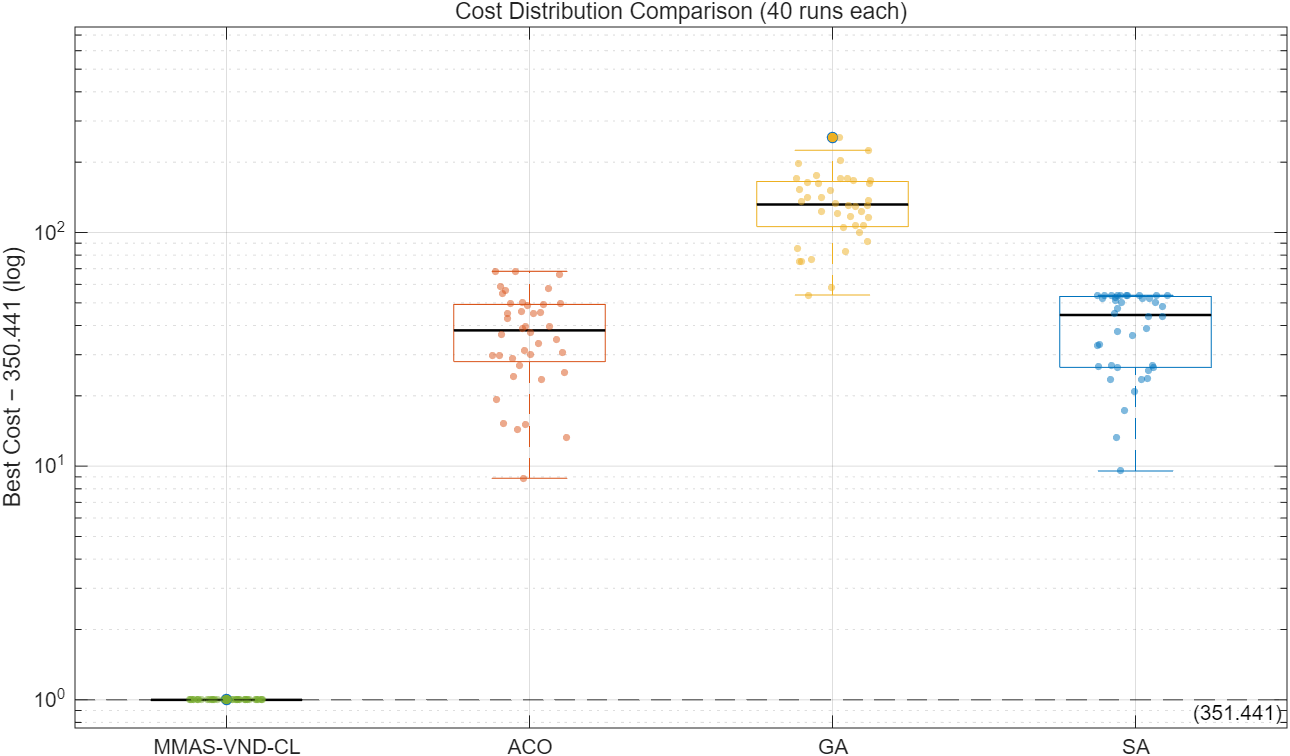
\includegraphics[width=0.3\textwidth]{figures/fig18a_tspbox_m1}}\hfil
\subfloat[Map~2]{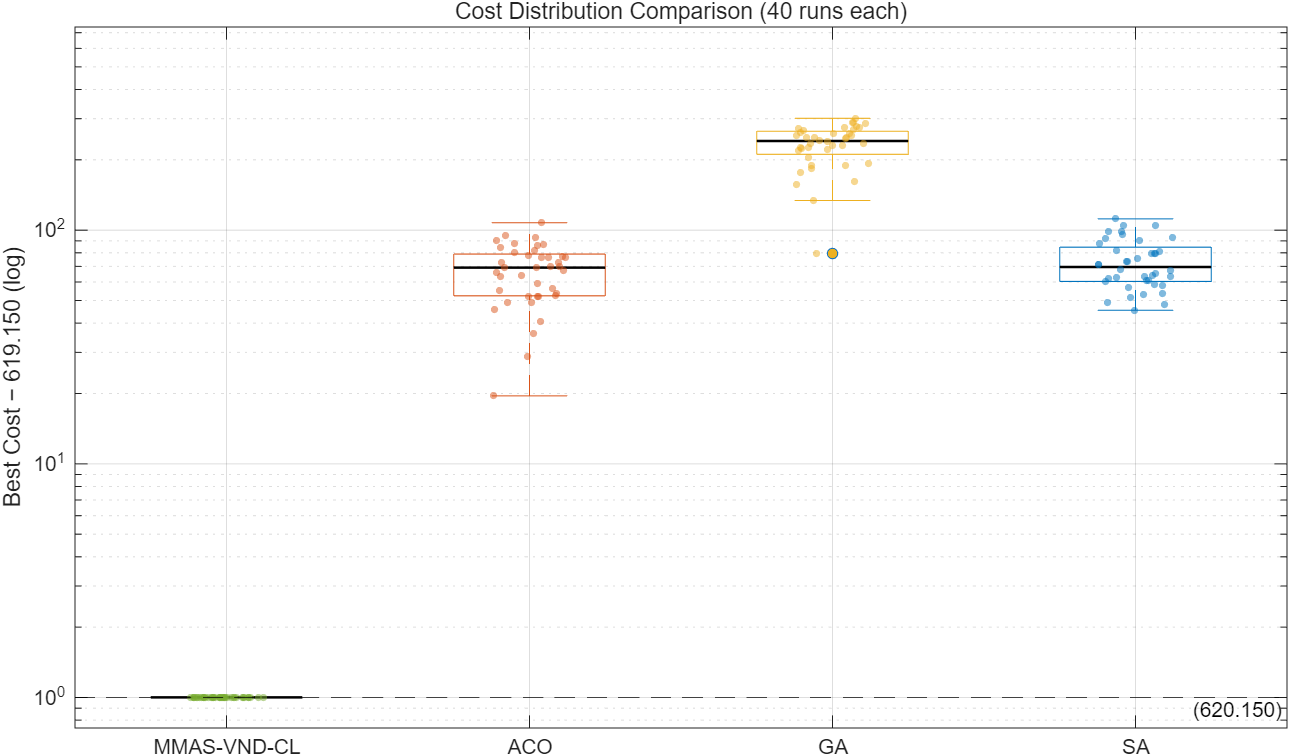
\includegraphics[width=0.3\textwidth]{figures/fig18b_tspbox_m2}}\hfil
\subfloat[kroB100]{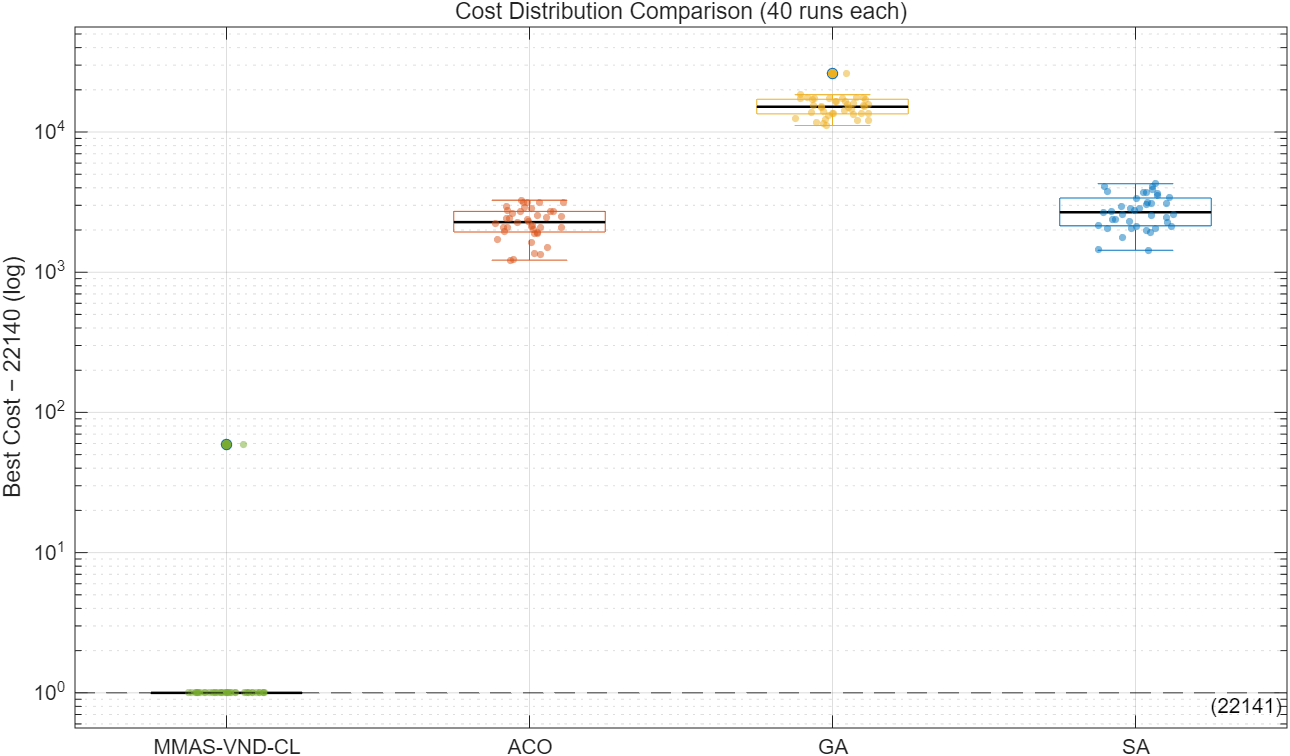
\includegraphics[width=0.3\textwidth]{figures/fig18c_tspbox_m3}}
\caption{四个旅行商求解器在三张地图上40次运行的代价分布（箱线图）。}
\label{fig:tsp_box}
\end{figure*}

\begin{figure*}[!t]

\centering
\subfloat[Map~1]{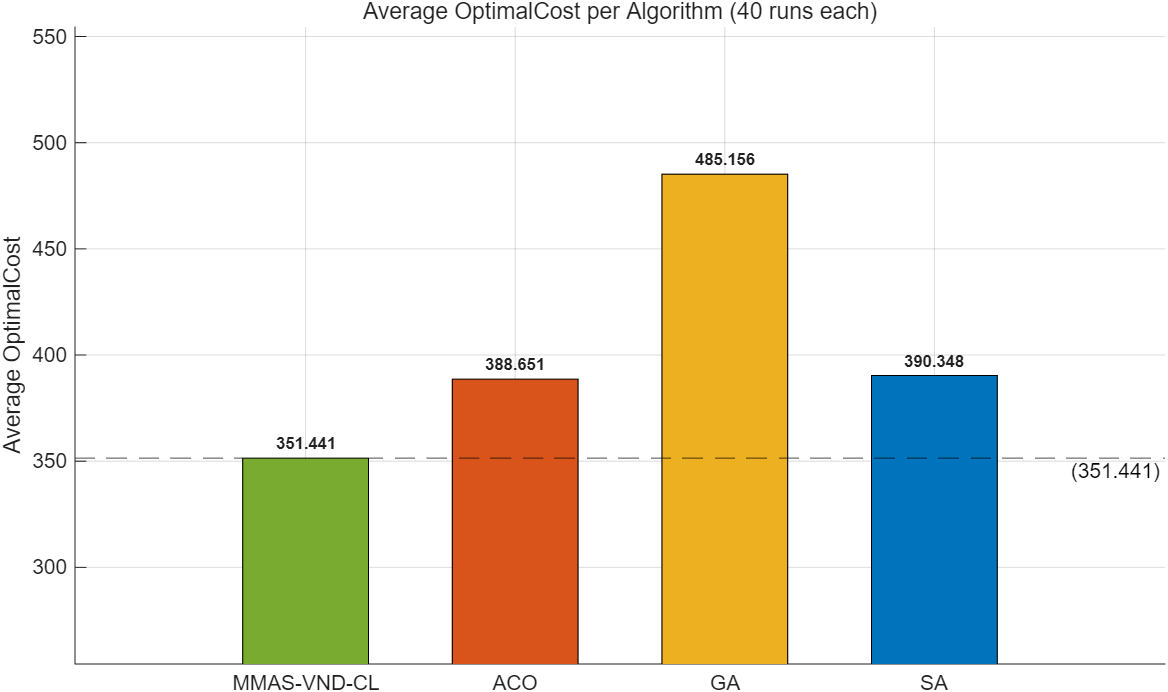
\includegraphics[width=0.3\textwidth]{figures/fig19a_tspcost_m1}}\hfil
\subfloat[Map~2]{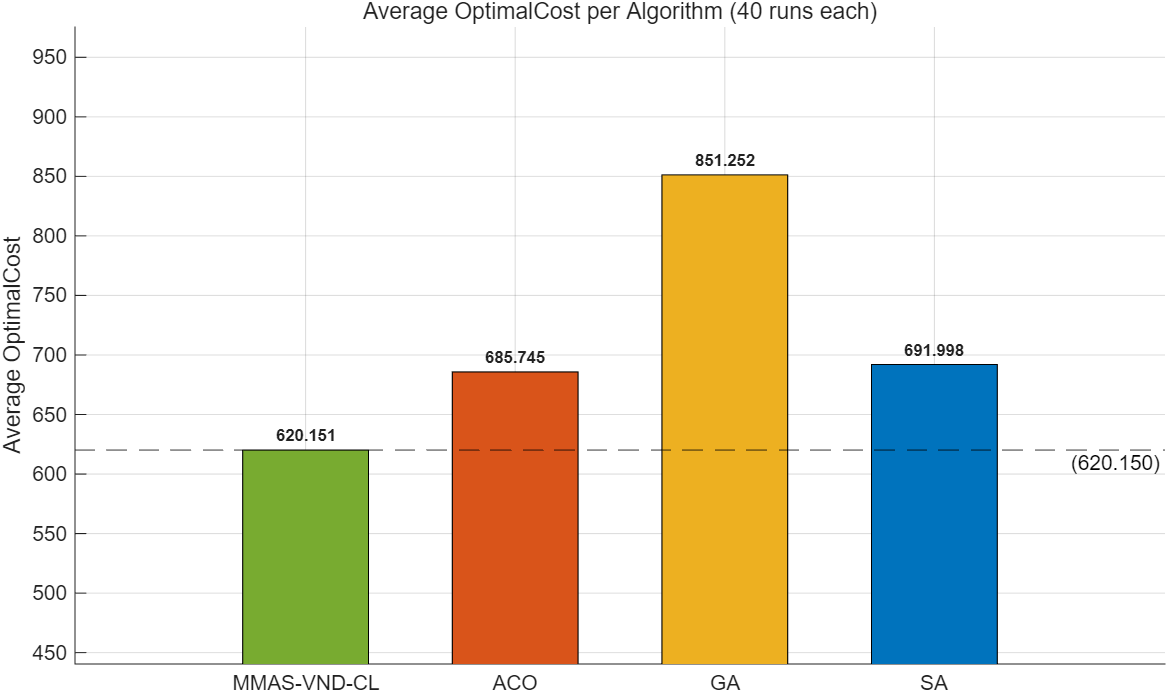
\includegraphics[width=0.3\textwidth]{figures/fig19b_tspcost_m2}}\hfil
\subfloat[kroB100]{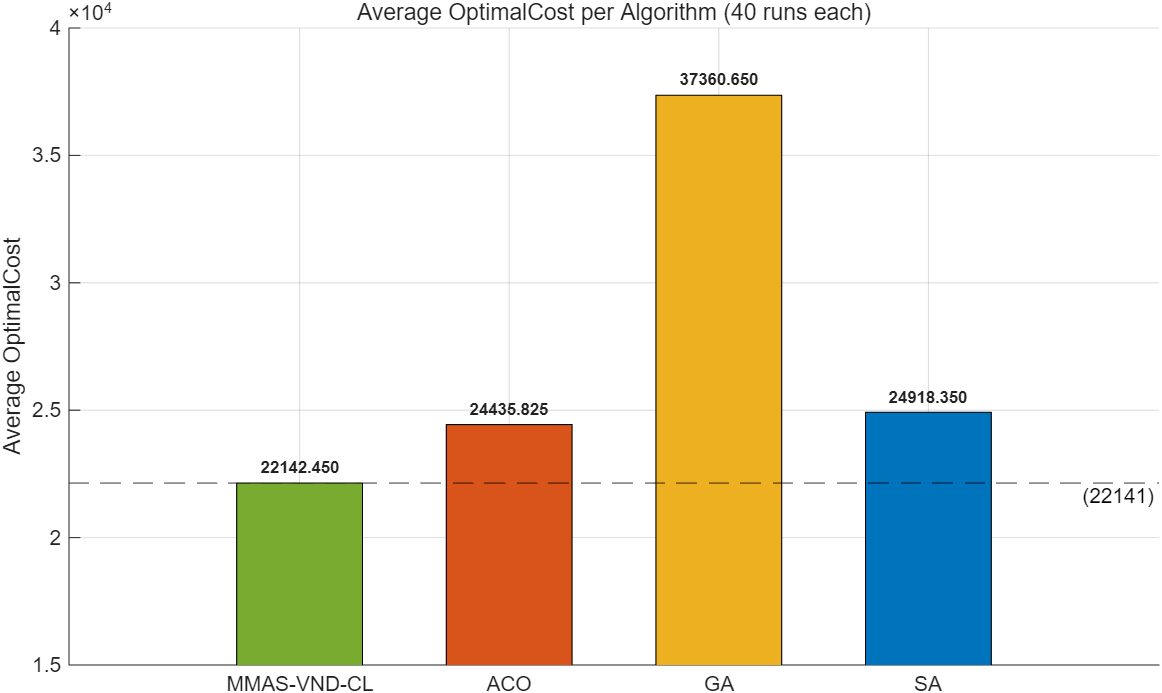
\includegraphics[width=0.3\textwidth]{figures/fig19c_tspcost_m3}}
\caption{四个旅行商求解器在三张地图上的平均代价对比（柱状图）。}
\label{fig:tsp_cost}
\end{figure*}

\begin{figure*}[!t]

\centering
\subfloat[Map~1]{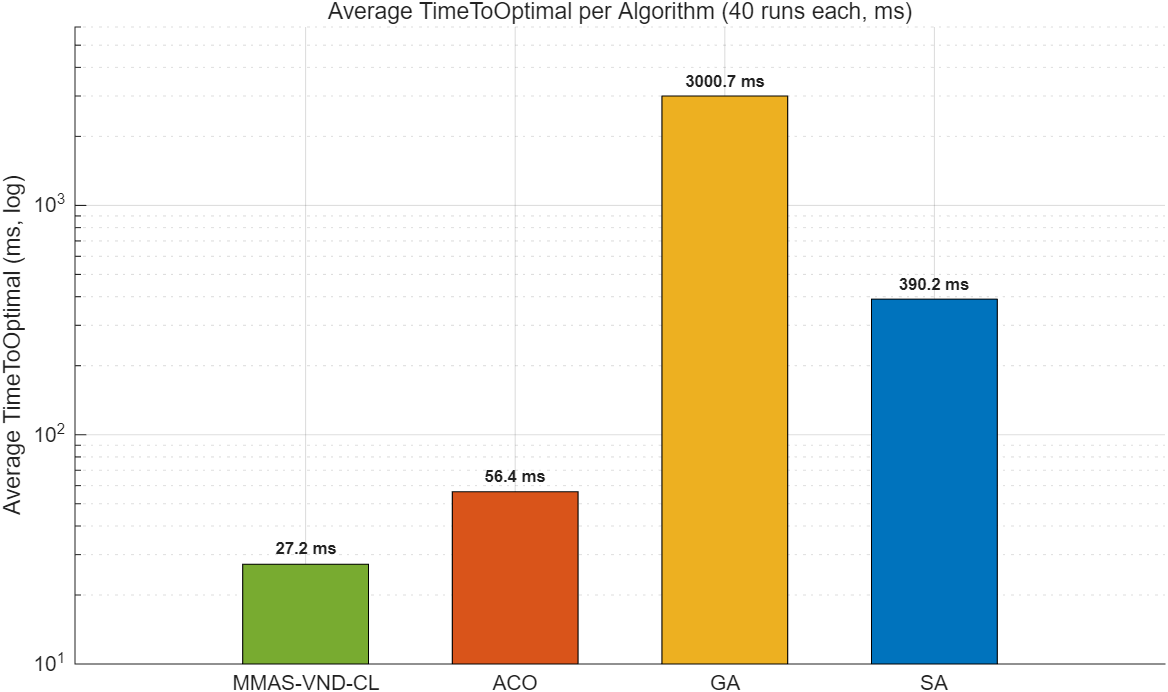
\includegraphics[width=0.3\textwidth]{figures/fig20a_tsptime_m1}}\hfil
\subfloat[Map~2]{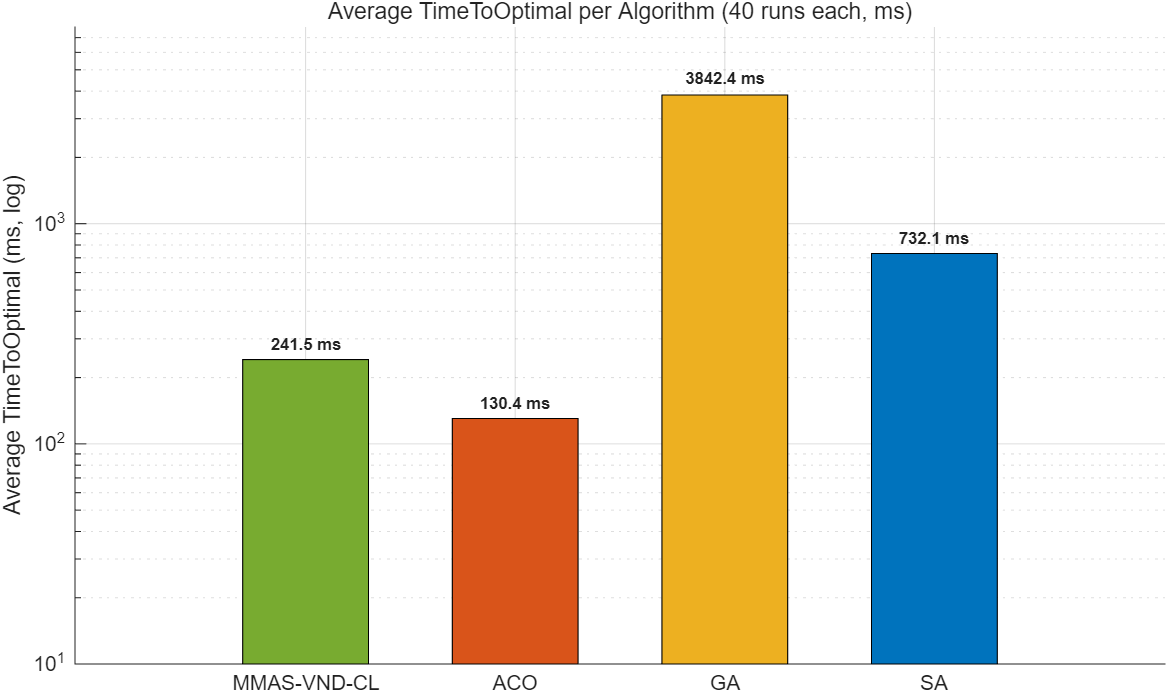
\includegraphics[width=0.3\textwidth]{figures/fig20b_tsptime_m2}}\hfil
\subfloat[kroB100]{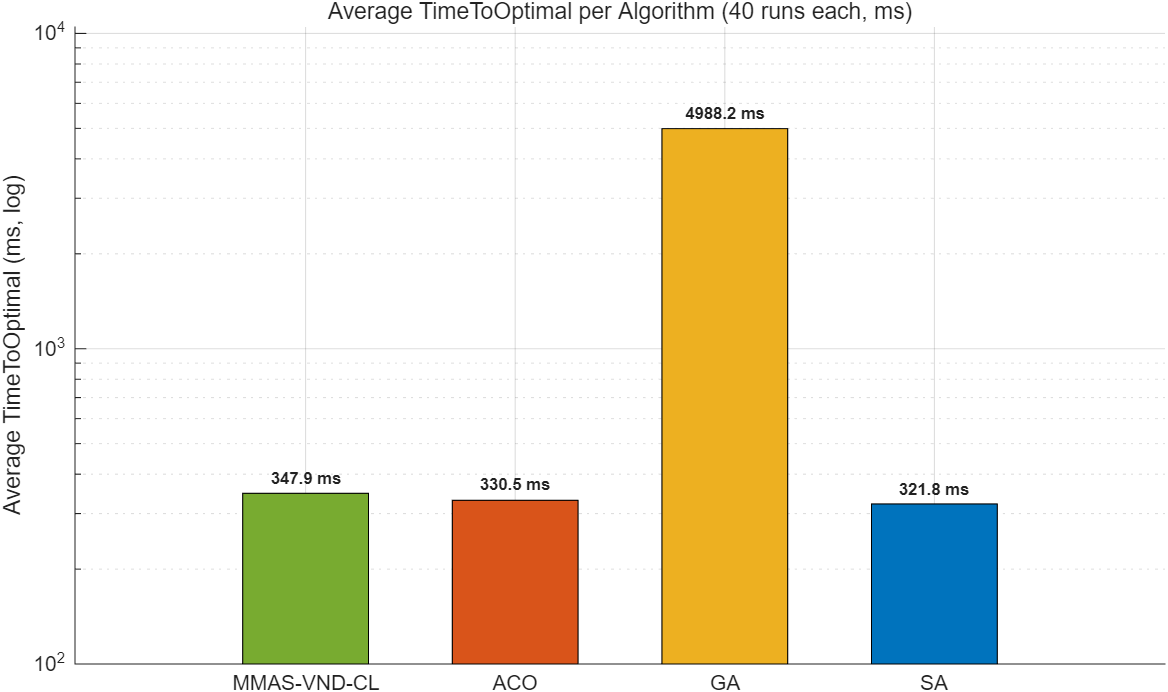
\includegraphics[width=0.3\textwidth]{figures/fig20c_tsptime_m3}}
\caption{四个旅行商求解器在三张地图上的平均计算时间对比（柱状图）。}
\label{fig:tsp_time}
\end{figure*}

\begin{figure*}[!t]

\centering
\subfloat[MMAS-VND-CL（本文）]{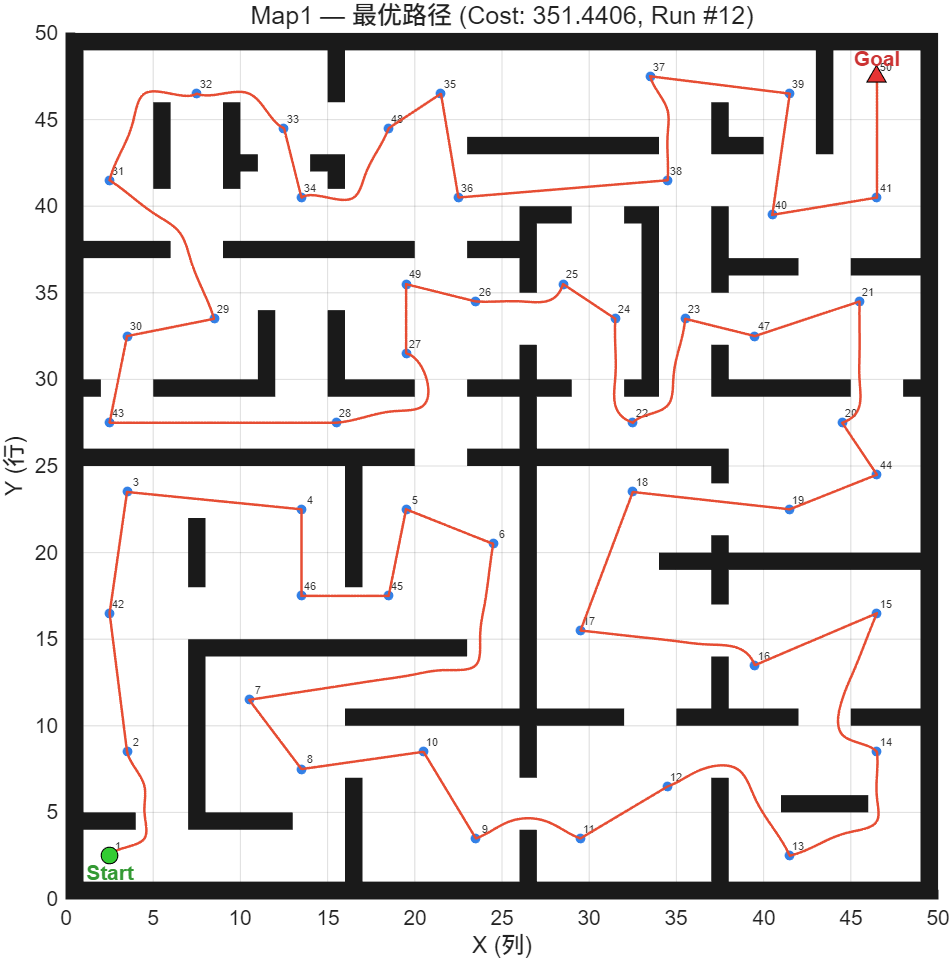
\includegraphics[width=0.22\textwidth]{figures/fig12_default_m1}\hfil
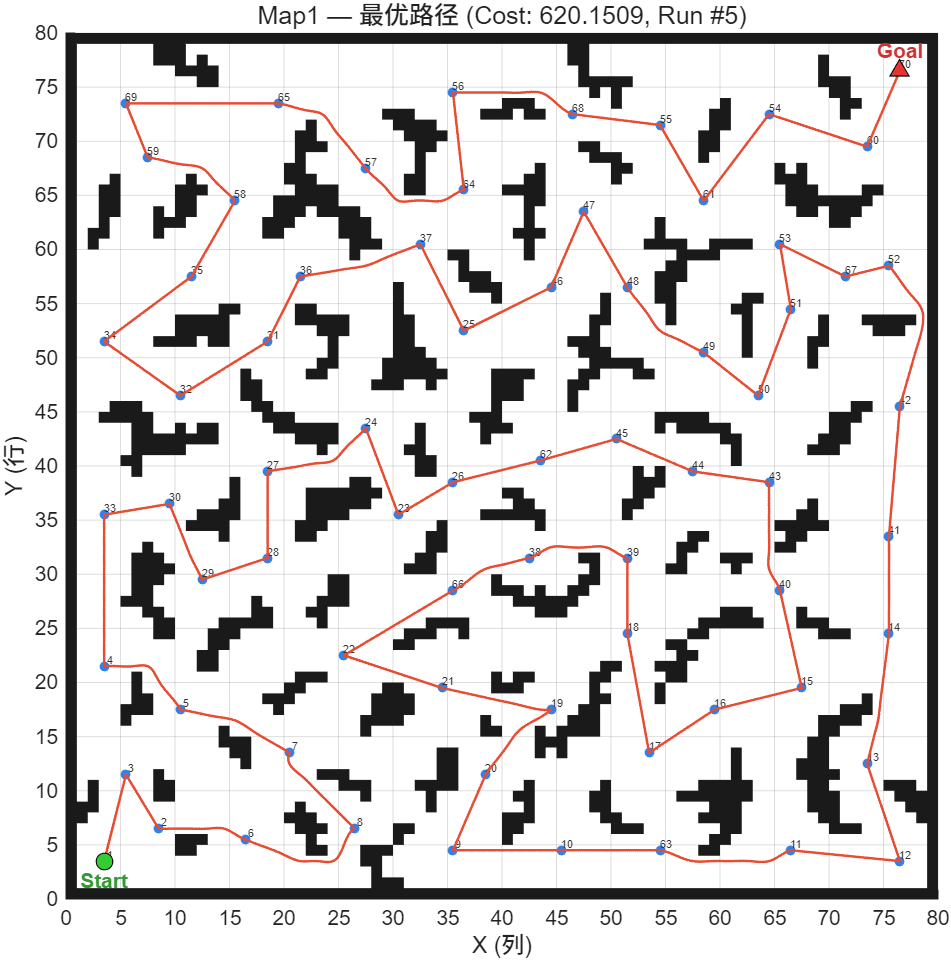
\includegraphics[width=0.22\textwidth]{figures/fig12_default_m2}\hfil
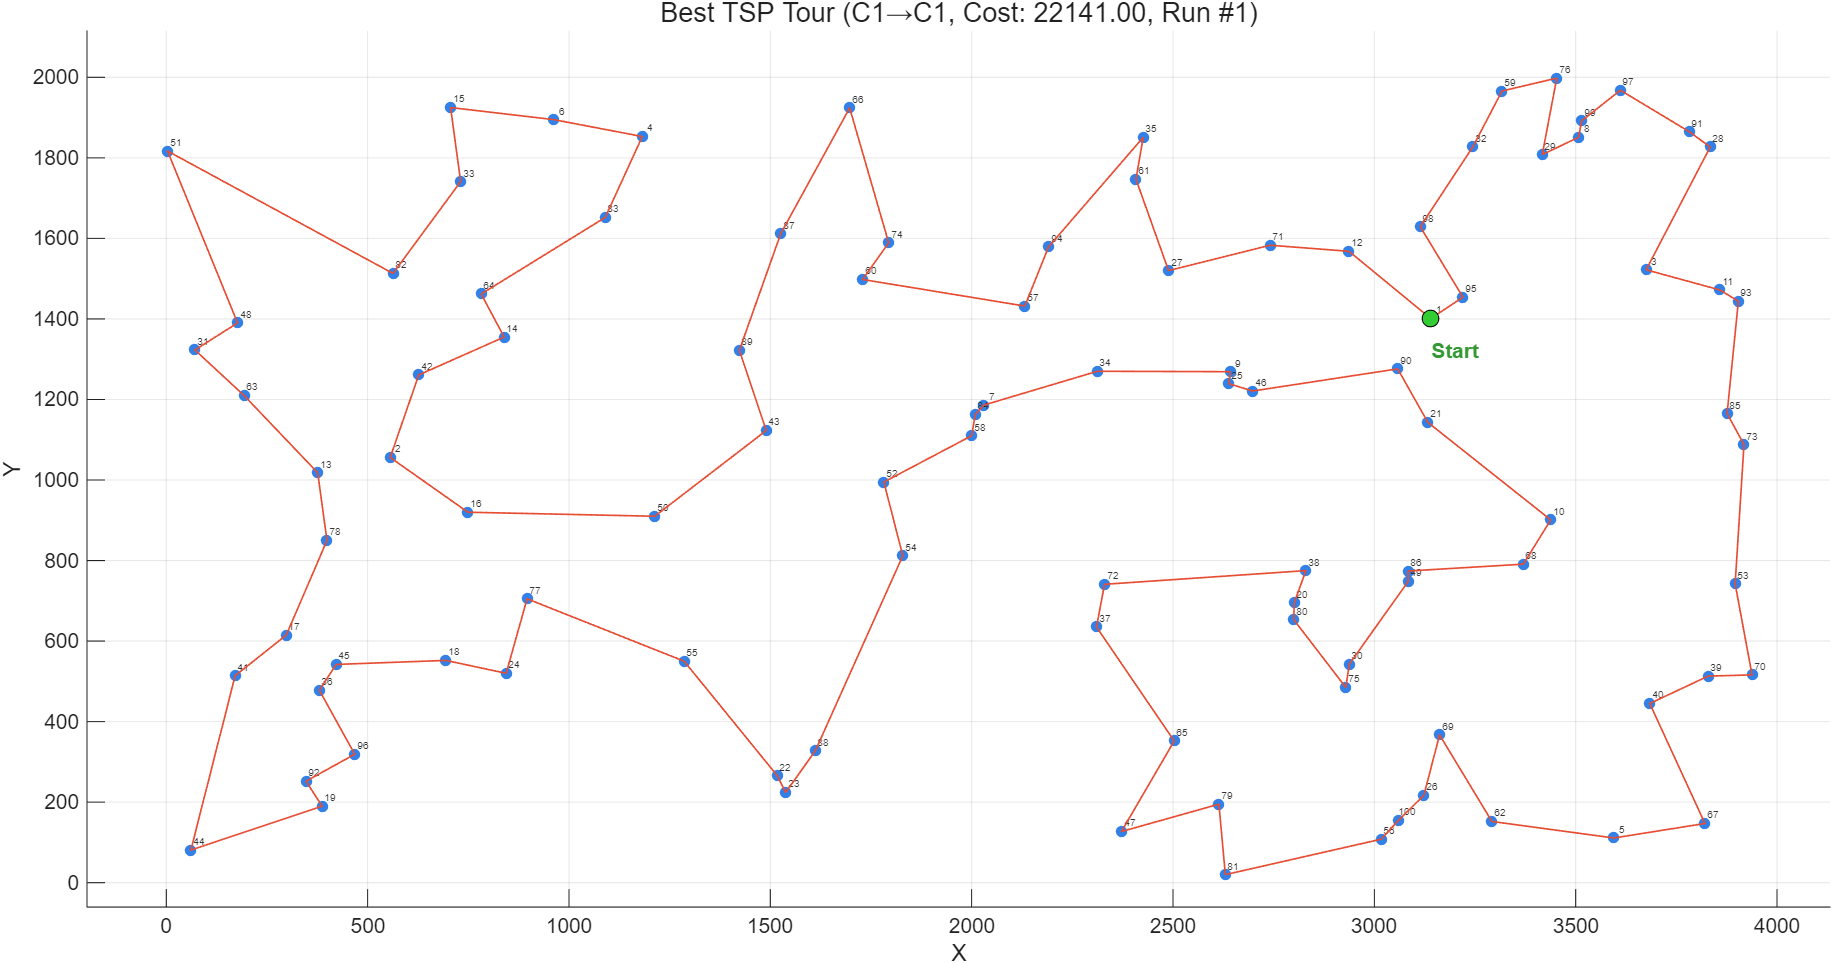
\includegraphics[width=0.22\textwidth]{figures/fig12_default_kro}}\\
\subfloat[ACO]{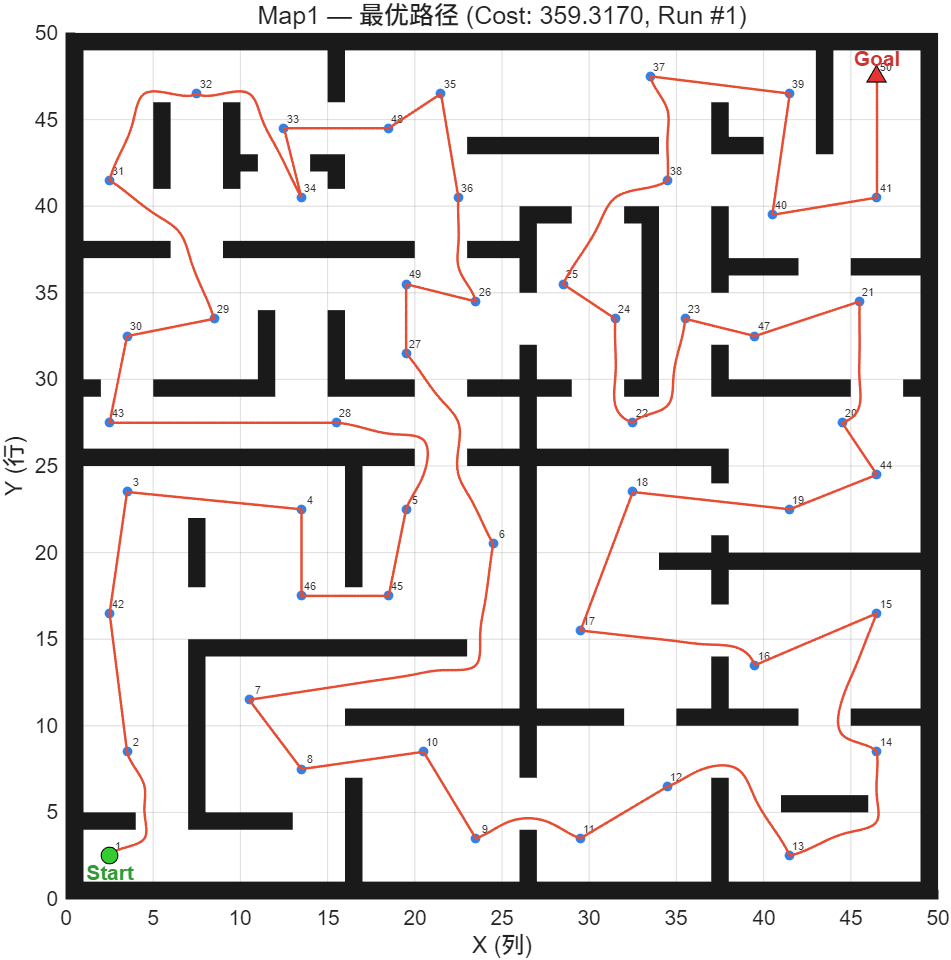
\includegraphics[width=0.22\textwidth]{figures/fig21b_aco_m1}\hfil
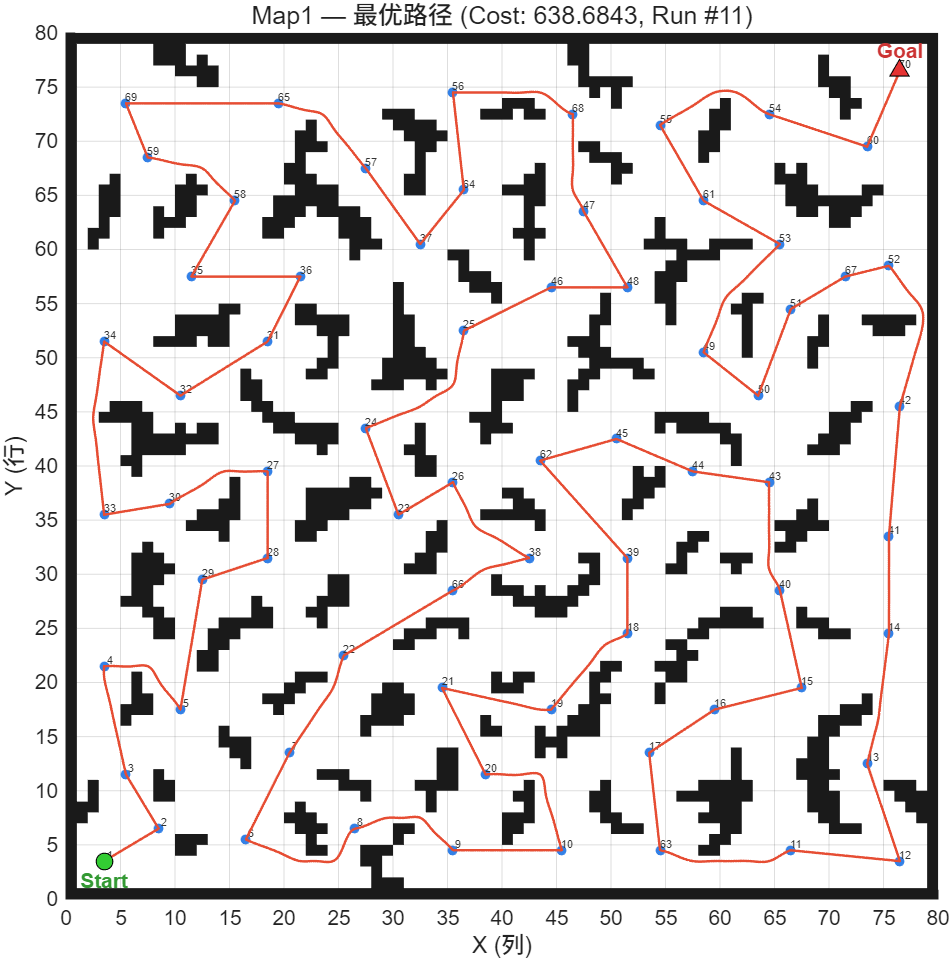
\includegraphics[width=0.22\textwidth]{figures/fig21b_aco_m2}\hfil
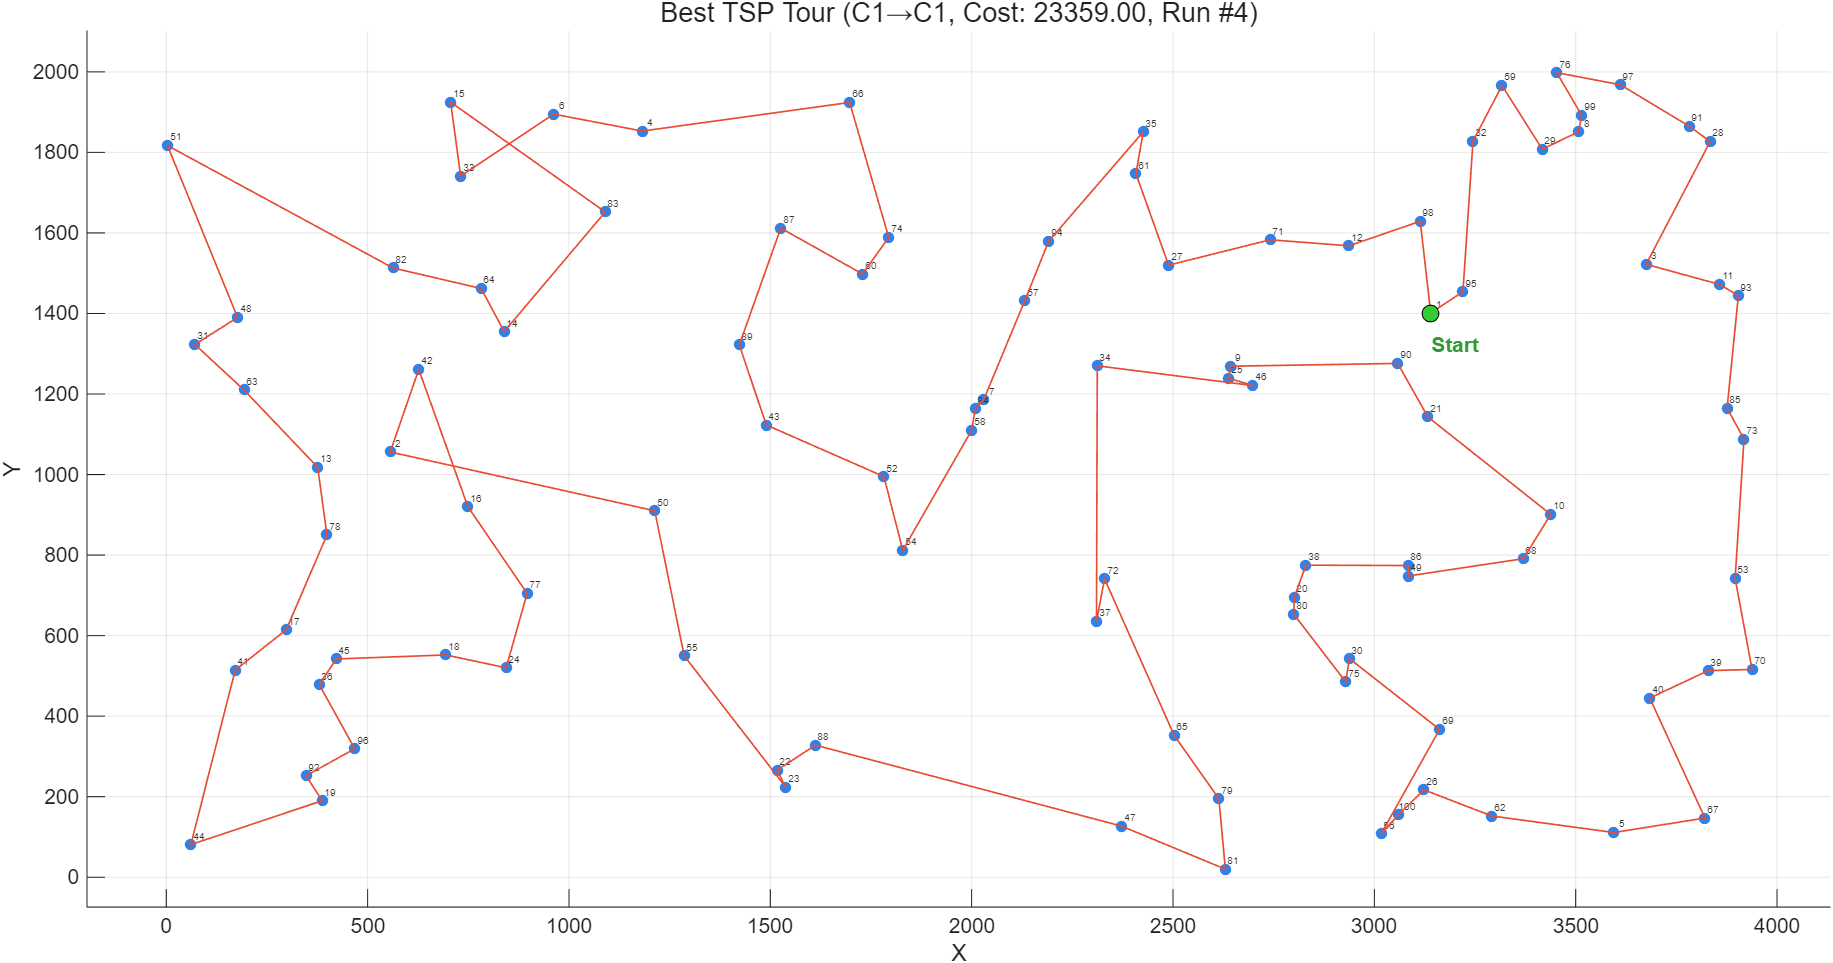
\includegraphics[width=0.22\textwidth]{figures/fig21b_aco_m3}}\\
\subfloat[GA]{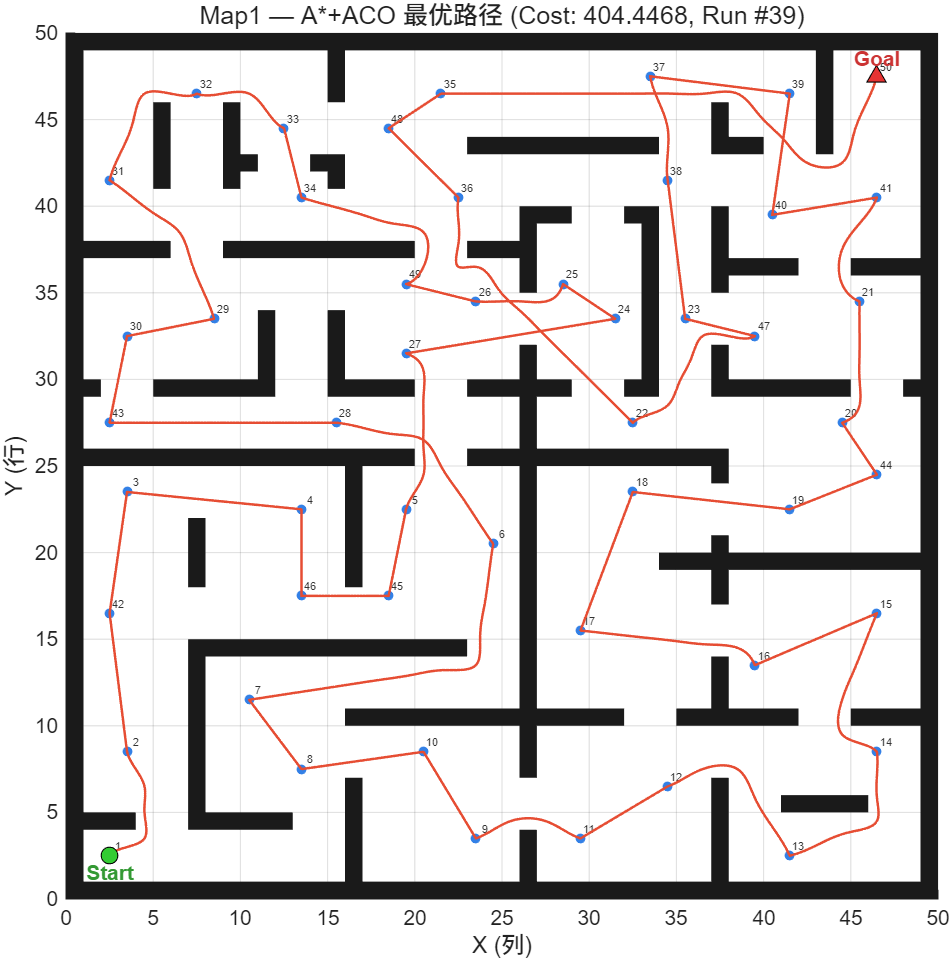
\includegraphics[width=0.22\textwidth]{figures/fig21c_ga_m1}\hfil
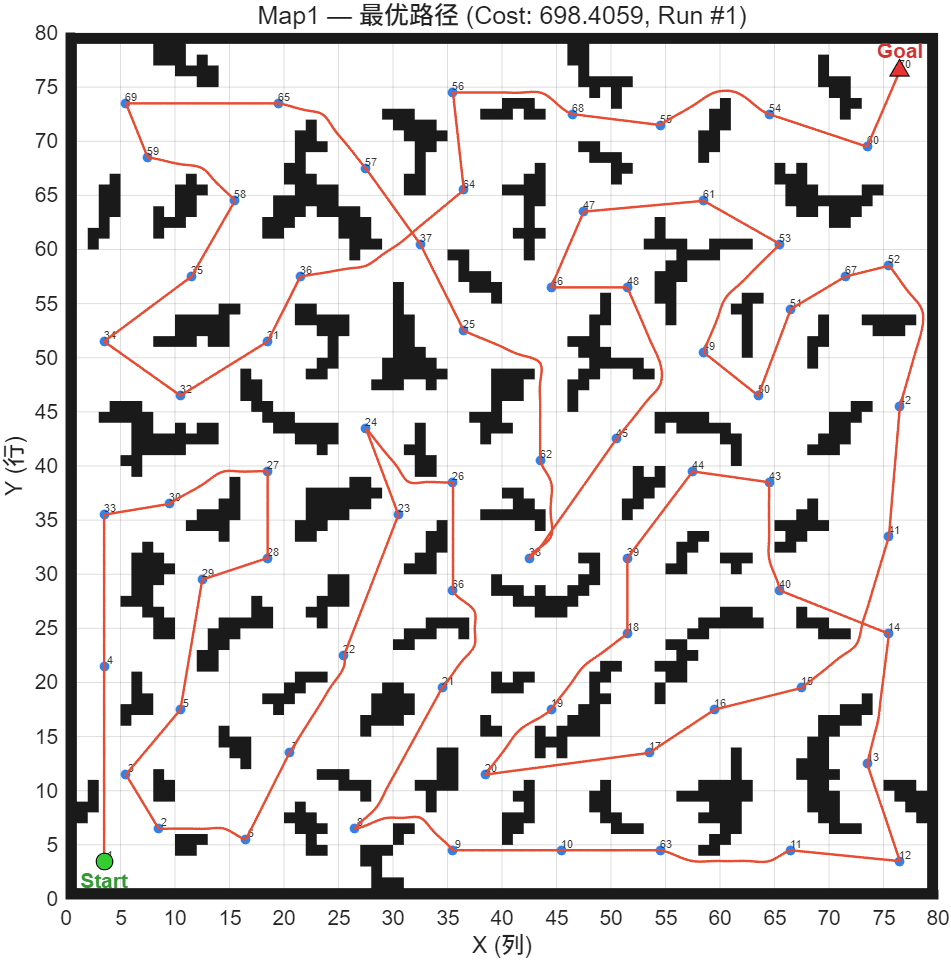
\includegraphics[width=0.22\textwidth]{figures/fig21c_ga_m2}\hfil
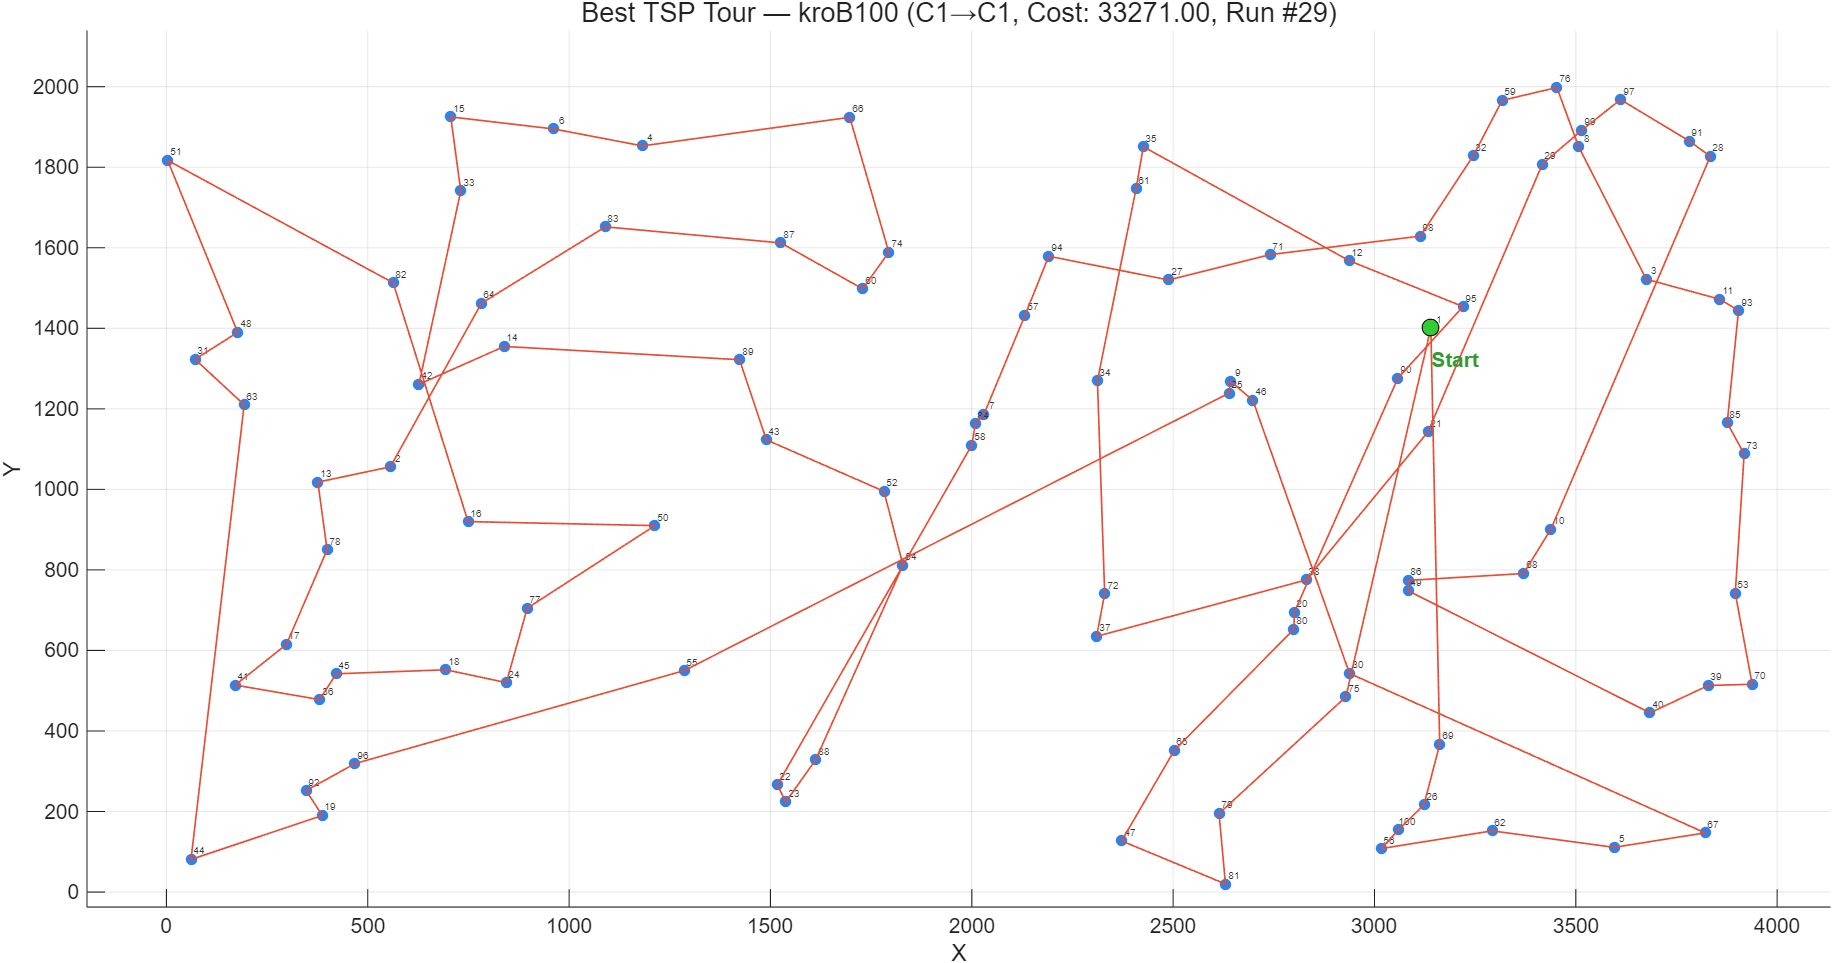
\includegraphics[width=0.22\textwidth]{figures/fig21c_ga_m3}}\\
\subfloat[SA]{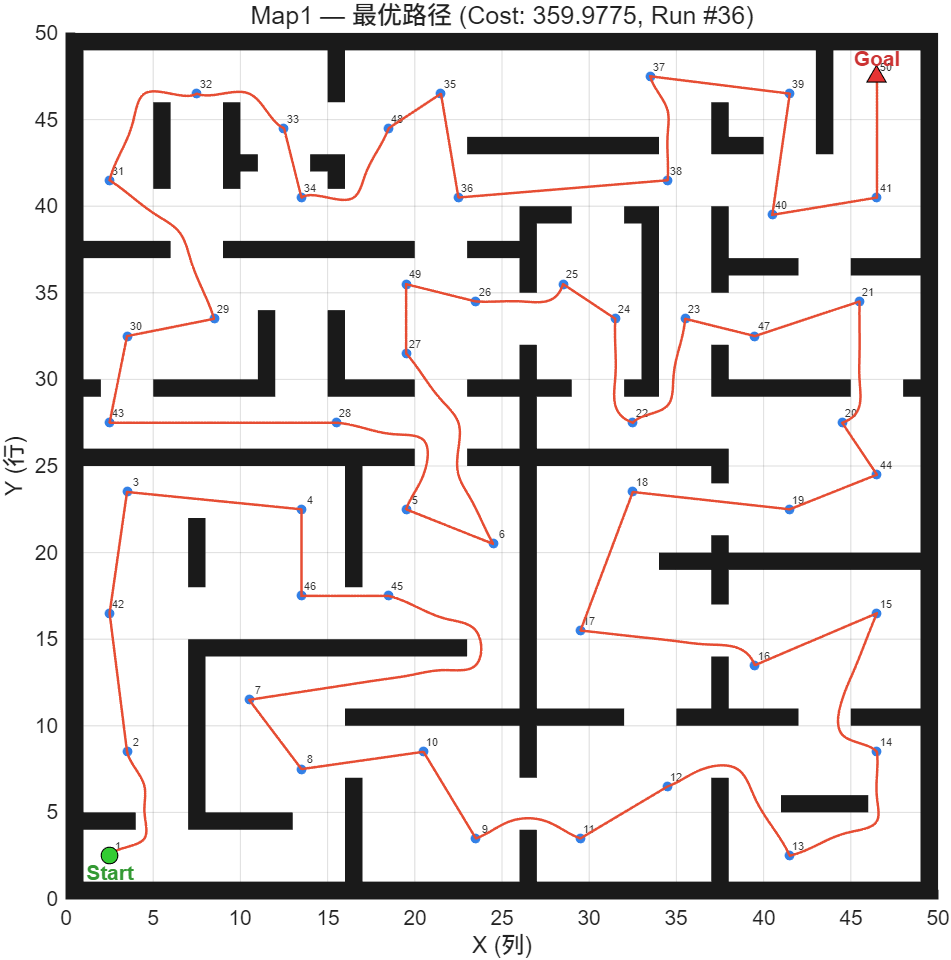
\includegraphics[width=0.22\textwidth]{figures/fig21d_sa_m1}\hfil
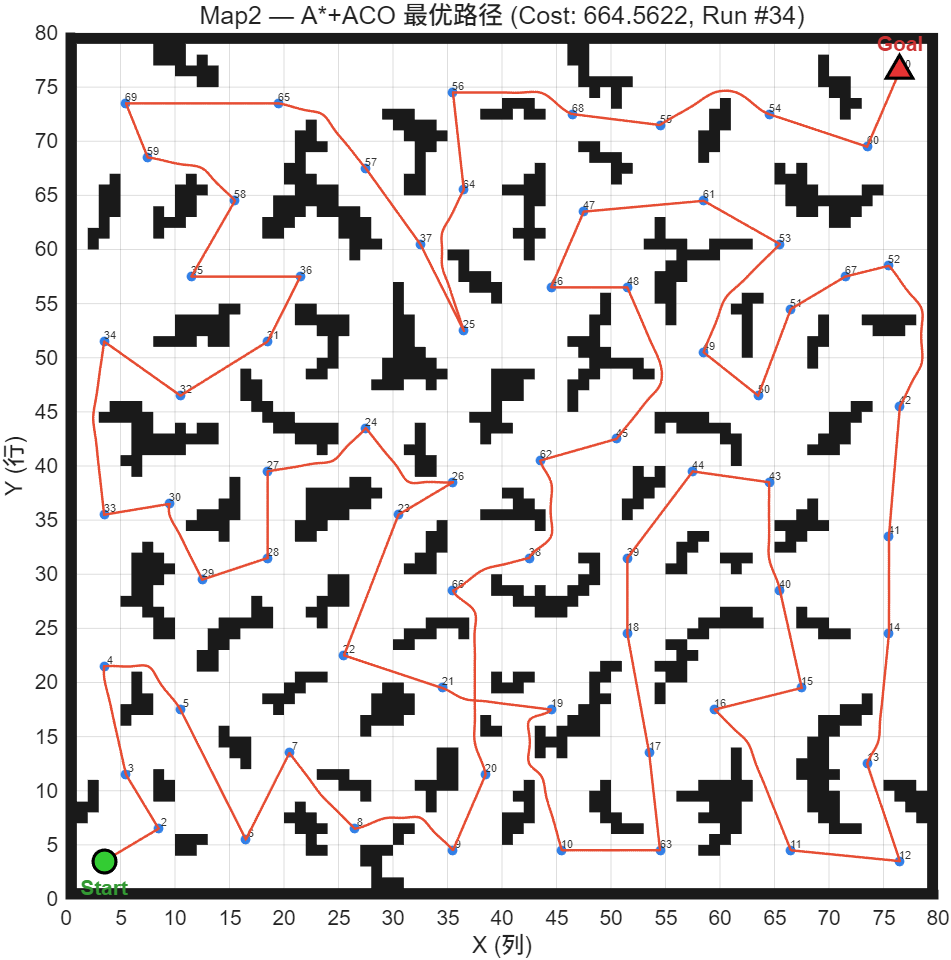
\includegraphics[width=0.22\textwidth]{figures/fig21d_sa_m2}\hfil
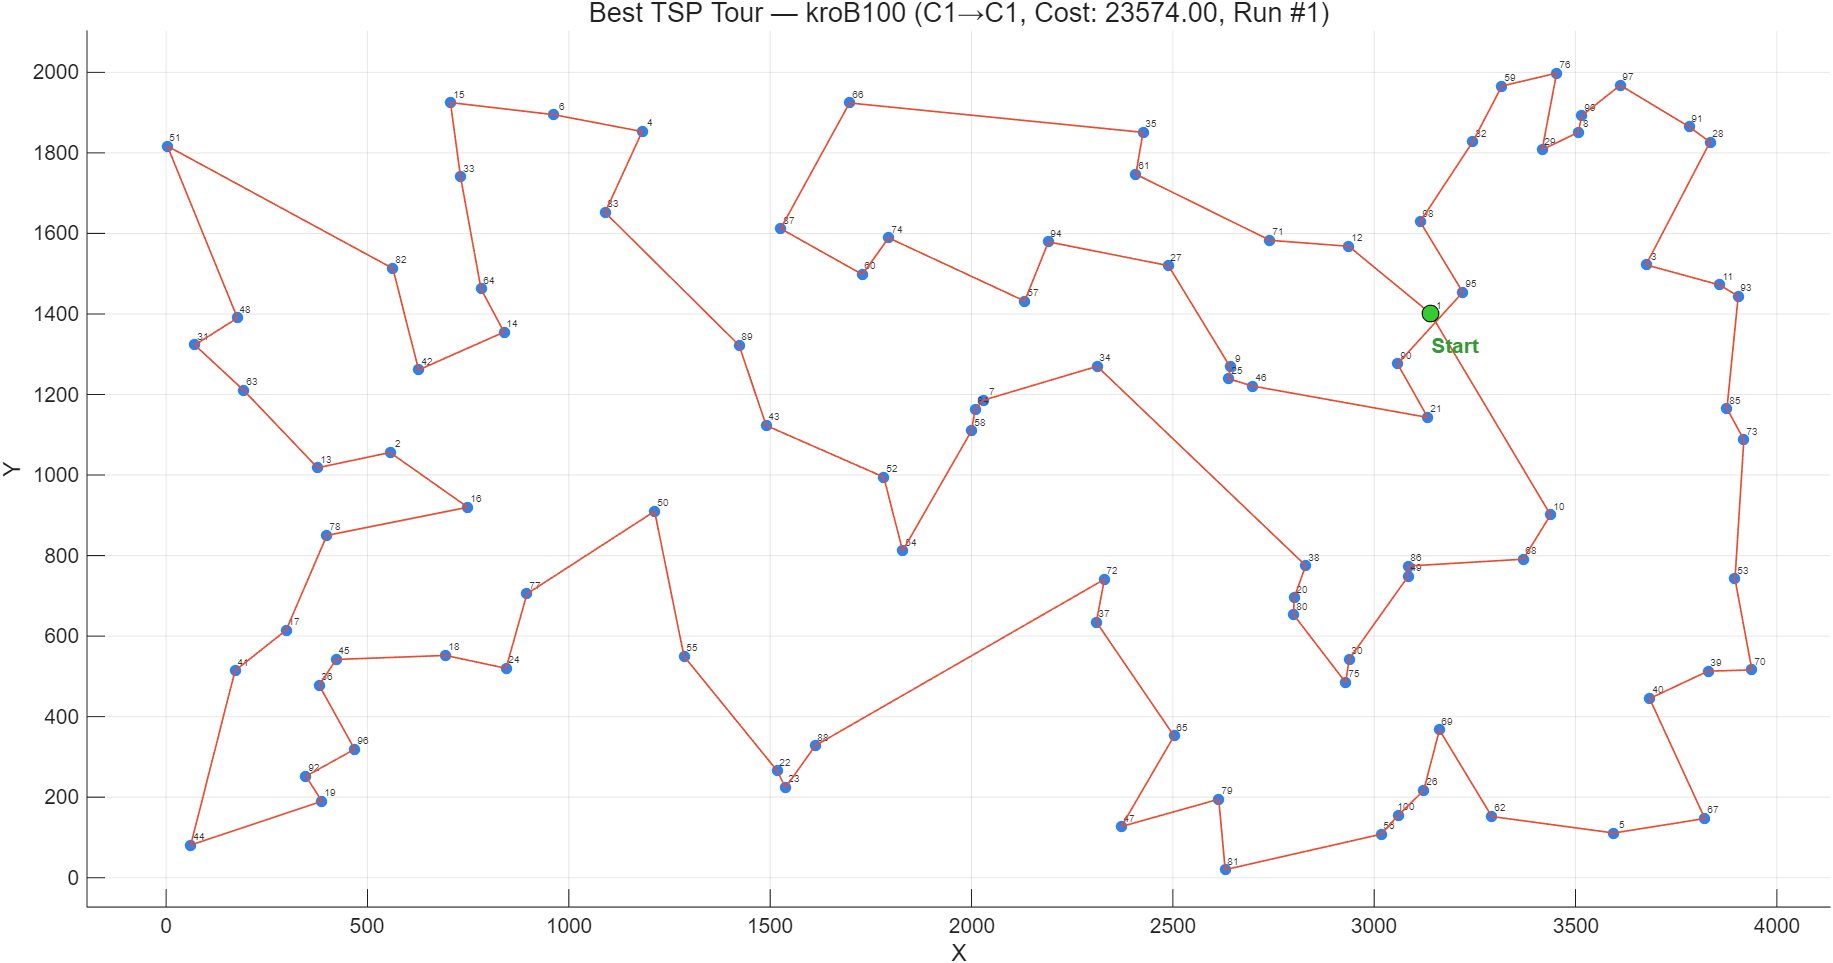
\includegraphics[width=0.22\textwidth]{figures/fig21d_sa_m3}}
\caption{每个旅行商求解器在三张地图上规划的最优代价路径图。每行从左至右依次为Map~1、Map~2、Map~3。}
\label{fig:tsp_paths}
\end{figure*}

\section{结论}

\label{sec:concl}

本文提出了一种面向障碍环境多目标点遍历路径规划的协同优化框架，将基于跳点搜索的改进A*全局规划器与面向开放旅行商问题的改进蚁群优化求解器相集成。该框架解决了文献中的一个实际空白：传统旅行商研究假设无约束的欧氏距离，而标准路径规划算法仅优化单对路由。通过全局规划器将障碍信息编码为代价矩阵，并通过蚁群优化求解器求解所得开放旅行商问题，该框架将几何推理与组合推理统一到单一管线中。

在路径规划方面，跳点搜索（JPS）利用均匀代价栅格地图中固有的对称性，剪枝冗余节点扩展，仅在最优路径改变方向或遇到强制选择的跳点处进行扩展。这大幅缩减了开阔环境中的搜索树规模，同时保持路径最优性。安全感知的路径简化通过四步流程——拐点提取、贪心正向扫描、中间点探索和路径对比——生成最小安全航点子集。弧长参数化三次样条平滑将简化折线转化为适合物理机器人执行的连续轨迹。

在旅行商优化方面，改进的蚁群优化求解器融合了六个集成机制。虚拟节点法将开放旅行商问题转化为标准闭环旅行商问题，使起点和终点能够完整参与信息素模型和局部搜索。具有动态边界的最大-最小蚁群系统信息素管理防止过早收敛并维持探索多样性。蚁群系统风格的伪随机转移规则通过受控贪心利用加速收敛。候选列表加速的可变邻域下降将局部搜索复杂度从$O(K^2)$降至$O(K \cdot k)$，使针对超过100个目标点问题的密集邻域搜索变得可行。S形渐进调度在迭代预算内将局部搜索从探索逐渐转向利用。基于种群同质性和最优解停滞的自适应停止准则，在进一步改进不太可能时终止搜索，节省计算资源。

实验结果验证了各组件的有效性。基于JPS的A*规划器相比Dijkstra和标准A*减少了多达83\%的节点扩展（Map~3上48个对比566个），搜索速度提升17倍（Map~2上11.85~ms对比202.29~ms），同时产生更短的路径。参数敏感性分析确认默认超参数代表均衡配置，其中贪心概率$q_0$和后期局部搜索比例$y_{\max}$是最敏感的参数。消融实验揭示了组件重要性的清晰层次：VND局部搜索和MMAS信息素边界是解质量的两大支柱——禁用任一组件将成功率从近100\%降至30\%以下——而伪随机转移规则、S曲线和候选列表主要贡献于收敛速度和计算效率。在多目标点遍历对比中，所提MMAS-VND-CL求解器在kroB100基准上以97.5\%的命中率达到最优代价（平均代价22142.45），比最优基线标准蚁群优化（平均代价24435.83）优10.4\%，同时标准差比遗传算法小60倍以上，展现出卓越的解质量和可靠性。

当前工作的若干局限性指明了未来研究方向。首先，框架假设静态且完全已知的障碍地图；扩展到任务执行期间出现或移动障碍物的动态环境需要在线重规划能力。其次，地图表示限于二维栅格地图；扩展到具有高程约束的三维地形将拓宽对空中和水下机器人的适用性。第三，候选列表大小$k$和其他蚁群优化超参数是固定的；自适应或基于学习的参数调优可进一步提升跨不同问题实例的性能。第四，框架目前处理单机器人任务；扩展到多机器人协同多目标点遍历——多个机器人共享目标工作量且必须避免机器人间碰撞——代表重要的实用泛化。最后，完整$O(N^2)$代价矩阵的计算对非常大的目标集变得昂贵；距离预言机近似或增量代价精化等技术可缓解此瓶颈。

\section*{致谢}

感谢相关实验环境与开源实现对本研究的支持（待补充具体致谢对象）。

\begin{thebibliography}{32}

\bibitem{ref1}

S.~B. Liu et al., ``SMUG planner: A safe multi-goal planner for mobile robots in challenging environments,'' \textit{IEEE Robot. Autom. Lett.}, vol.~8, no.~9, pp.~5504--5511, 2023.

\bibitem{ref2}

H.~T.~T. Binh, ``Fast marching firework method for multi-goal mobile robot path planning in complex obstacle maps,'' \textit{Intell. Service Robot.}, vol.~18, 2025, doi: 10.1007/s11370-025-00654-6.

\bibitem{ref3}

C.-G. Wu, Y.-C. Liang, H.-P. Lee, C. Lu, and C. Lin, ``Solving constrained traveling salesman problems by genetic algorithms,'' \textit{Prog. Nat. Sci.}, vol.~14, no.~7, pp.~631--637, 2004.

\bibitem{ref4}

``A survey on approximability of traveling salesman problems using the TSP-T3CO definition scheme,'' \textit{Ann. Oper. Res.}, 2025, doi: 10.1007/s10479-025-06641-5.

\bibitem{ref5}

P.~E. Hart, N.~J. Nilsson, and B. Raphael, ``A formal basis for the heuristic determination of minimum cost paths,'' \textit{IEEE Trans. Syst. Sci. Cybern.}, vol.~4, no.~2, pp.~100--107, 1968.

\bibitem{ref6}

E.~W. Dijkstra, ``A note on two problems in connexion with graphs,'' \textit{Numer. Math.}, vol.~1, no.~1, pp.~269--271, 1959.

\bibitem{ref7}

S.~M. LaValle, ``Rapidly-exploring random trees: A new tool for path planning,'' Dept. Comput. Sci., Iowa State Univ., Ames, IA, USA, Tech. Rep. 98-11, 1998.

\bibitem{ref8}

``A comprehensive review of improved A* path planning algorithms and their hybrid integrations,'' \textit{Automation}, vol.~6, p.~52, 2025.

\bibitem{ref9}

L.~H. O. Rios and L. Chaimowicz, ``A survey and classification of A* based best-first heuristic search algorithms,'' in \textit{Proc. 20th Brazilian Symp. Artif. Intell. (SBIA)}, 2010, pp.~253--262.

\bibitem{ref10}

M. Likhachev, G. Gordon, and S. Thrun, ``ARA*: Anytime A* with provable bounds on sub-optimality,'' in \textit{Adv. Neural Inf. Process. Syst. (NIPS)}, 2003, pp.~767--774.

\bibitem{ref11}

D. Harabor and A. Grastien, ``Online graph pruning for pathfinding on grid maps,'' in \textit{Proc. 25th AAAI Conf. Artif. Intell. (AAAI-11)}, 2011, pp.~1114--1119.

\bibitem{ref12}

D. Harabor and A. Grastien, ``Improving jump point search,'' in \textit{Proc. 24th Int. Conf. Automated Planning Scheduling (ICAPS-14)}, 2014, pp.~128--135.

\bibitem{ref13}

``Improved JPS and DWA path planning algorithm for mobile robots,'' \textit{Expert Syst. Appl.}, 2026.

\bibitem{ref14}

``Research on mobile robot path planning based on an improved bidirectional jump point search algorithm,'' \textit{Electronics}, vol.~14, no.~8, p.~1669, 2025, doi: 10.3390/electronics14081669.

\bibitem{ref15}

``Adaptive weight optimization based jump point Theta* algorithm in mobile robot path planning for intricate environments,'' \textit{Discover Appl. Sci.}, vol.~7, p.~11, 2025, doi: 10.1007/s42452-025-07932-z.

\bibitem{ref16}

``UGV path optimization in UAV-assisted environments using visibility-aware path simplification,'' \textit{J. Sens. Actuator Netw.}, vol.~15, no.~3, p.~41, 2025.

\bibitem{ref17}

``Enhancing the safety and smoothness of path planning through an integration of Dijkstra's algorithm and piecewise cubic Bezier optimization,'' \textit{Expert Syst. Appl.}, 2025.

\bibitem{ref18}

``Adaptive A*/NSGA-II framework for multi-goal navigation of mobile robots,'' \textit{Meas. Sci. Technol.}, 2025, doi: 10.1088/1361-6501/ae9209.

\bibitem{ref19}

J.~H. Holland, \textit{Adaptation in Natural and Artificial Systems}. Ann Arbor, MI, USA: Univ. Michigan Press, 1975.

\bibitem{ref20}

S. Kirkpatrick, C.~D. Gelatt, and M.~P. Vecchi, ``Optimization by simulated annealing,'' \textit{Science}, vol.~220, no.~4598, pp.~671--680, 1983.

\bibitem{ref21}

M. Dorigo, V. Maniezzo, and A. Colorni, ``Ant system: Optimization by a colony of cooperating agents,'' \textit{IEEE Trans. Syst., Man, Cybern. B}, vol.~26, no.~1, pp.~29--41, 1996.

\bibitem{ref22}

M. Dorigo and L.~M. Gambardella, ``Ant colony system: A cooperative learning approach to the traveling salesman problem,'' \textit{IEEE Trans. Evol. Comput.}, vol.~1, no.~1, pp.~53--66, 1997.

\bibitem{ref23}

T. St\"utzle and H.~H. Hoos, ``MAX--MIN ant system,'' \textit{Future Gener. Comput. Syst.}, vol.~16, no.~8, pp.~889--914, 2000.

\bibitem{ref24}

P. Hansen and N. Mladenovi\'c, ``Variable neighborhood search: Principles and applications,'' \textit{Eur. J. Oper. Res.}, vol.~130, no.~3, pp.~449--467, 2001.

\bibitem{ref25}

N.~A. Kyriakakis, M. Marinaki, and Y. Marinakis, ``A hybrid ant colony optimization--variable neighborhood descent approach for the cumulative capacitated vehicle routing problem,'' \textit{Comput. Oper. Res.}, vol.~134, p.~105397, 2021.

\bibitem{ref26}

``An improvement to the 2-opt heuristic algorithm for approximation of optimal TSP tour,'' \textit{Appl. Sci.}, vol.~13, no.~12, p.~7339, 2023, doi: 10.3390/app13127339.

\bibitem{ref27}

``Matrix-based ant colony system for traveling salesman problem,'' in \textit{Proc. IEEE Int. Conf. Syst., Man, Cybern. (SMC)}, 2024.

\bibitem{ref28}

``nLKH-ACS: A niching Lin-Kernighan--Helsgaun-based ant colony system for multisolution traveling salesman problems,'' \textit{IEEE Trans. Evol. Comput.}, 2024.

\bibitem{ref29}

``CAACS: A carbon aware ant colony system,'' \textit{Sci. Rep.}, 2025.

\bibitem{ref30}

``Ant colony optimization for multiple traveling salesmen problem with revisitable cities,'' in \textit{Proc. IEEE}, 2024.

\bibitem{ref31}

B. Yao, Q. Hu, L. Zhang, and J. Tian, ``Improved ant colony optimization for seafood product delivery routing problem,'' \textit{Promet--Traffic Transp.}, vol.~26, no.~1, 2014.

\bibitem{ref32}

B. Yao, C. Chen, X. Song, and X. Yang, ``Fresh seafood delivery routing problem using an improved ant colony optimization,'' \textit{Ann. Oper. Res.}, vol.~273, no.~1--2, pp.~163--186, 2019, doi: 10.1007/s10479-017-2531-2.

\end{thebibliography}

\end{document}

